\documentclass[12pt]{tufte-book}
%DIF LATEXDIFF DIFFERENCE FILE
%DIF DEL notes-F24-old.tex   Tue Nov  5 23:59:23 2024
%DIF ADD notes-F24.tex       Tue Nov  5 23:51:00 2024
\usepackage{amsthm,amssymb,amsmath,thmtools,datetime,tikz}
\setcounter{secnumdepth}{3}

\declaretheorem[numberwithin=chapter,shaded={bgcolor=Lavender}]{definition}

\declaretheorem[numberwithin=chapter,shaded={bgcolor=Thistle}]{lemma}
\declaretheorem[numberwithin=chapter,shaded={bgcolor=Thistle}]{claim}

\declaretheorem[numberwithin=chapter,shaded={bgcolor=Apricot}]{theorem}

\declaretheorem[numberwithin=chapter,shaded={bgcolor=yellow}]{remark}
\declaretheorem[numberwithin=chapter]{exercise}
\declaretheorem[numberwithin=chapter,shaded={bgcolor=pink}]{construction}
\usepackage[
    type={CC},
    modifier={by-nc-nd},
    version={4.0},
]{doclicense}

\usepackage{graphicx,xcolor,mdframed}
%\usepackage[version=0.96]{pgf}
\usepackage{enumitem}


\def\chpcolor{blue!45}
\def\chpcolortxt{blue!60}

\iffalse
\titleformat{\chapter}%
  {\huge\rmfamily\itshape\color{red}}% format applied to label+text
  {\llap{\colorbox{red}{\parbox{1.5cm}{\hfill\itshape\huge\color{white}\thechapter}}}}% label
  {2pt}% horizontal separation between label and title body
  {}% before the title body
  []% after the title body
\fi

\hypersetup{colorlinks}% uncomment this line if you prefer colored hyperlinks (e.g., for onscreen viewing)

%%
% Book metadata
\title{A Course in Theory of Cryptography}
\author[Sanjam Garg]{Sanjam Garg}
%\publisher{Publisher of This Book}

%%
% If they're installed, use Bergamo and Chantilly from www.fontsite.com.
% They're clones of Bembo and Gill Sans, respectively.
%\IfFileExists{bergamo.sty}{\usepackage[osf]{bergamo}}{}% Bembo
%\IfFileExists{chantill.sty}{\usepackage{chantill}}{}% Gill Sans

%\usepackage{microtype}

%%
% Just some sample text
\usepackage{lipsum}
\newcommand{\ma}{\mathcal{A}}
\newcommand{\cA}{\mathcal{A}}
\newcommand{\mb}{\mathcal{B}}
\newcommand{\cB}{\mathcal{B}}

\newcommand{\getsr}{\xleftarrow{\$}}
\newcommand{\bit}{\{0,1\}}

\newcommand{\Gen}{\mathsf{Gen}}
\newcommand{\gen}{\mathsf{Gen}}
\newcommand{\Enc}{\mathsf{Enc}}
% \newcommand{\enc}{\mathsf{Enc}}
\newcommand{\Dec}{\mathsf{Dec}}
% \newcommand{\dec}{\mathsf{Dec}}
% \newcommand{\pk}{\mathsf{pk}}
% \newcommand{\sk}{\mathsf{sk}}
\newcommand{\ek}{\mathsf{ek}}

% \newcommand{\concat}[0]{\; || \;}

% \newcommand{\bin}{\{0,1\}}
% \newcommand{\adv}{\mathcal{A}}
% \newcommand{\advb}{\mathcal{B}}
% \newcommand{\advc}{\mathcal{C}}
% \newcommand{\fake}{\mathsf{FAKE}}

\newcommand{\Sign}{\mathsf{Sign}}
\newcommand{\Verify}{\mathsf{Verify}}
%\newcommand{\negl}{\mathsf{negl}}
\newcommand{\abort}{\mathsf{abort}}
\newcommand{\Sampler}{\mathsf{Sampler}}
\newcommand{\Eval}{\mathsf{Eval}}
\renewcommand{\tag}{\mathsf{tag}}
\newcommand{\PRF}{\mathsf{PRF}}
\newcommand{\LWE}{\mathsf{LWE}}
%%
% For nicely typeset tabular material
\usepackage{booktabs}

\usepackage[n,advantage,operators,sets,adversary,landau,probability,notions,logic,ff,mm,primitives,events,complexity,oracles,asymptotics,keys]{cryptocode} 
%%
% For graphics / images
\usepackage{graphicx,algpseudocode}
\setkeys{Gin}{width=\linewidth,totalheight=\textheight,keepaspectratio}
\graphicspath{{graphics/}}

% The fancyvrb package lets us customize the formatting of verbatim
% environments.  We use a slightly smaller font.
\usepackage{fancyvrb}
\fvset{fontsize=\normalsize}

%%
% Prints argument within hanging parentheses (i.e., parentheses that take
% up no horizontal space).  Useful in tabular environments.
\newcommand{\hangp}[1]{\makebox[0pt][r]{(}#1\makebox[0pt][l]{)}}

%%
% Prints an asterisk that takes up no horizontal space.
% Useful in tabular environments.
\newcommand{\hangstar}{\makebox[0pt][l]{*}}

%%
% Prints a trailing space in a smart way.
\usepackage{xspace}

%%
% Some shortcuts for Tufte's book titles.  The lowercase commands will
% produce the initials of the book title in italics.  The all-caps commands
% will print out the full title of the book in italics.
\newcommand{\vdqi}{\textit{VDQI}\xspace}
\newcommand{\ei}{\textit{EI}\xspace}
\newcommand{\ve}{\textit{VE}\xspace}
\newcommand{\be}{\textit{BE}\xspace}
\newcommand{\VDQI}{\textit{The Visual Display of Quantitative Information}\xspace}
\newcommand{\EI}{\textit{Envisioning Information}\xspace}
\newcommand{\VE}{\textit{Visual Explanations}\xspace}
\newcommand{\BE}{\textit{Beautiful Evidence}\xspace}

\newcommand{\TL}{Tufte-\LaTeX\xspace}

% Prints the month name (e.g., January) and the year (e.g., 2008)
\newcommand{\monthyear}{%
  \ifcase\month\or January\or February\or March\or April\or May\or June\or
  July\or August\or September\or October\or November\or
  December\fi\space\number\year
}


% Prints an epigraph and speaker in sans serif, all-caps type.
\newcommand{\openepigraph}[2]{%
  %\sffamily\fontsize{14}{16}\selectfont
  \begin{fullwidth}
  \sffamily\large
  \begin{doublespace}
  \noindent\allcaps{#1}\\% epigraph
  \noindent\allcaps{#2}% author
  \end{doublespace}
  \end{fullwidth}
}

% Inserts a blank page
\newcommand{\blankpage}{\newpage\hbox{}\thispagestyle{empty}\newpage}

\usepackage{units}

% Typesets the font size, leading, and measure in the form of 10/12x26 pc.
\newcommand{\measure}[3]{#1/#2$\times$\unit[#3]{pc}}

% Macros for typesetting the documentation
\newcommand{\hlred}[1]{\textcolor{Maroon}{#1}}% prints in red
\newcommand{\hangleft}[1]{\makebox[0pt][r]{#1}}
\newcommand{\hairsp}{\hspace{1pt}}% hair space
\newcommand{\hquad}{\hskip0.5em\relax}% half quad space
\newcommand{\TODO}{\textcolor{red}{\bf TODO!}\xspace}
\newcommand{\ie}{\textit{i.\hairsp{}e.}\xspace}
\newcommand{\eg}{\textit{e.\hairsp{}g.}\xspace}
\newcommand{\na}{\quad--}% used in tables for N/A cells
\providecommand{\XeLaTeX}{X\lower.5ex\hbox{\kern-0.15em\reflectbox{E}}\kern-0.1em\LaTeX}
\newcommand{\tXeLaTeX}{\XeLaTeX\index{XeLaTeX@\protect\XeLaTeX}}
% \index{\texttt{\textbackslash xyz}@\hangleft{\texttt{\textbackslash}}\texttt{xyz}}
\newcommand{\tuftebs}{\symbol{'134}}% a backslash in tt type in OT1/T1
\newcommand{\doccmdnoindex}[2][]{\texttt{\tuftebs#2}}% command name -- adds backslash automatically (and doesn't add cmd to the index)
\newcommand{\doccmddef}[2][]{%
  \hlred{\texttt{\tuftebs#2}}\label{cmd:#2}%
  \ifthenelse{\isempty{#1}}%
    {% add the command to the index
      \index{#2 command@\protect\hangleft{\texttt{\tuftebs}}\texttt{#2}}% command name
    }%
    {% add the command and package to the index
      \index{#2 command@\protect\hangleft{\texttt{\tuftebs}}\texttt{#2} (\texttt{#1} package)}% command name
      \index{#1 package@\texttt{#1} package}\index{packages!#1@\texttt{#1}}% package name
    }%
}% command name -- adds backslash automatically
\newcommand{\doccmd}[2][]{%
  \texttt{\tuftebs#2}%
  \ifthenelse{\isempty{#1}}%
    {% add the command to the index
      \index{#2 command@\protect\hangleft{\texttt{\tuftebs}}\texttt{#2}}% command name
    }%
    {% add the command and package to the index
      \index{#2 command@\protect\hangleft{\texttt{\tuftebs}}\texttt{#2} (\texttt{#1} package)}% command name
      \index{#1 package@\texttt{#1} package}\index{packages!#1@\texttt{#1}}% package name
    }%
}% command name -- adds backslash automatically
\newcommand{\docopt}[1]{\ensuremath{\langle}\textrm{\textit{#1}}\ensuremath{\rangle}}% optional command argument
\newcommand{\docarg}[1]{\textrm{\textit{#1}}}% (required) command argument
\newenvironment{docspec}{\begin{quotation}\ttfamily\parskip0pt\parindent0pt\ignorespaces}{\end{quotation}}% command specification environment
\newcommand{\docenv}[1]{\texttt{#1}\index{#1 environment@\texttt{#1} environment}\index{environments!#1@\texttt{#1}}}% environment name
\newcommand{\docenvdef}[1]{\hlred{\texttt{#1}}\label{env:#1}\index{#1 environment@\texttt{#1} environment}\index{environments!#1@\texttt{#1}}}% environment name
\newcommand{\docpkg}[1]{\texttt{#1}\index{#1 package@\texttt{#1} package}\index{packages!#1@\texttt{#1}}}% package name
\newcommand{\doccls}[1]{\texttt{#1}}% document class name
\newcommand{\docclsopt}[1]{\texttt{#1}\index{#1 class option@\texttt{#1} class option}\index{class options!#1@\texttt{#1}}}% document class option name
\newcommand{\docclsoptdef}[1]{\hlred{\texttt{#1}}\label{clsopt:#1}\index{#1 class option@\texttt{#1} class option}\index{class options!#1@\texttt{#1}}}% document class option name defined
\newcommand{\docmsg}[2]{\bigskip\begin{fullwidth}\noindent\ttfamily#1\end{fullwidth}\medskip\par\noindent#2}
\newcommand{\docfilehook}[2]{\texttt{#1}\index{file hooks!#2}\index{#1@\texttt{#1}}}
\newcommand{\doccounter}[1]{\texttt{#1}\index{#1 counter@\texttt{#1} counter}}

% Generates the index
\usepackage{makeidx}
\makeindex
%DIF PREAMBLE EXTENSION ADDED BY LATEXDIFF
%DIF UNDERLINE PREAMBLE %DIF PREAMBLE
\RequirePackage[normalem]{ulem} %DIF PREAMBLE
\RequirePackage{color}\definecolor{RED}{rgb}{1,0,0}\definecolor{BLUE}{rgb}{0,0,1} %DIF PREAMBLE
\providecommand{\DIFadd}[1]{{\protect\color{blue}\uwave{#1}}} %DIF PREAMBLE
\providecommand{\DIFdel}[1]{{\protect\color{red}\sout{#1}}}                      %DIF PREAMBLE
%DIF SAFE PREAMBLE %DIF PREAMBLE
\providecommand{\DIFaddbegin}{} %DIF PREAMBLE
\providecommand{\DIFaddend}{} %DIF PREAMBLE
\providecommand{\DIFdelbegin}{} %DIF PREAMBLE
\providecommand{\DIFdelend}{} %DIF PREAMBLE
\providecommand{\DIFmodbegin}{} %DIF PREAMBLE
\providecommand{\DIFmodend}{} %DIF PREAMBLE
%DIF FLOATSAFE PREAMBLE %DIF PREAMBLE
\providecommand{\DIFaddFL}[1]{\DIFadd{#1}} %DIF PREAMBLE
\providecommand{\DIFdelFL}[1]{\DIFdel{#1}} %DIF PREAMBLE
\providecommand{\DIFaddbeginFL}{} %DIF PREAMBLE
\providecommand{\DIFaddendFL}{} %DIF PREAMBLE
\providecommand{\DIFdelbeginFL}{} %DIF PREAMBLE
\providecommand{\DIFdelendFL}{} %DIF PREAMBLE
\newcommand{\DIFscaledelfig}{0.5}
%DIF HIGHLIGHTGRAPHICS PREAMBLE %DIF PREAMBLE
\RequirePackage{settobox} %DIF PREAMBLE
\RequirePackage{letltxmacro} %DIF PREAMBLE
\newsavebox{\DIFdelgraphicsbox} %DIF PREAMBLE
\newlength{\DIFdelgraphicswidth} %DIF PREAMBLE
\newlength{\DIFdelgraphicsheight} %DIF PREAMBLE
% store original definition of \includegraphics %DIF PREAMBLE
\LetLtxMacro{\DIFOincludegraphics}{\includegraphics} %DIF PREAMBLE
\newcommand{\DIFaddincludegraphics}[2][]{{\color{blue}\fbox{\DIFOincludegraphics[#1]{#2}}}} %DIF PREAMBLE
\newcommand{\DIFdelincludegraphics}[2][]{% %DIF PREAMBLE
\sbox{\DIFdelgraphicsbox}{\DIFOincludegraphics[#1]{#2}}% %DIF PREAMBLE
\settoboxwidth{\DIFdelgraphicswidth}{\DIFdelgraphicsbox} %DIF PREAMBLE
\settoboxtotalheight{\DIFdelgraphicsheight}{\DIFdelgraphicsbox} %DIF PREAMBLE
\scalebox{\DIFscaledelfig}{% %DIF PREAMBLE
\parbox[b]{\DIFdelgraphicswidth}{\usebox{\DIFdelgraphicsbox}\\[-\baselineskip] \rule{\DIFdelgraphicswidth}{0em}}\llap{\resizebox{\DIFdelgraphicswidth}{\DIFdelgraphicsheight}{% %DIF PREAMBLE
\setlength{\unitlength}{\DIFdelgraphicswidth}% %DIF PREAMBLE
\begin{picture}(1,1)% %DIF PREAMBLE
\thicklines\linethickness{2pt} %DIF PREAMBLE
{\color[rgb]{1,0,0}\put(0,0){\framebox(1,1){}}}% %DIF PREAMBLE
{\color[rgb]{1,0,0}\put(0,0){\line( 1,1){1}}}% %DIF PREAMBLE
{\color[rgb]{1,0,0}\put(0,1){\line(1,-1){1}}}% %DIF PREAMBLE
\end{picture}% %DIF PREAMBLE
}\hspace*{3pt}}} %DIF PREAMBLE
} %DIF PREAMBLE
\LetLtxMacro{\DIFOaddbegin}{\DIFaddbegin} %DIF PREAMBLE
\LetLtxMacro{\DIFOaddend}{\DIFaddend} %DIF PREAMBLE
\LetLtxMacro{\DIFOdelbegin}{\DIFdelbegin} %DIF PREAMBLE
\LetLtxMacro{\DIFOdelend}{\DIFdelend} %DIF PREAMBLE
\DeclareRobustCommand{\DIFaddbegin}{\DIFOaddbegin \let\includegraphics\DIFaddincludegraphics} %DIF PREAMBLE
\DeclareRobustCommand{\DIFaddend}{\DIFOaddend \let\includegraphics\DIFOincludegraphics} %DIF PREAMBLE
\DeclareRobustCommand{\DIFdelbegin}{\DIFOdelbegin \let\includegraphics\DIFdelincludegraphics} %DIF PREAMBLE
\DeclareRobustCommand{\DIFdelend}{\DIFOaddend \let\includegraphics\DIFOincludegraphics} %DIF PREAMBLE
\LetLtxMacro{\DIFOaddbeginFL}{\DIFaddbeginFL} %DIF PREAMBLE
\LetLtxMacro{\DIFOaddendFL}{\DIFaddendFL} %DIF PREAMBLE
\LetLtxMacro{\DIFOdelbeginFL}{\DIFdelbeginFL} %DIF PREAMBLE
\LetLtxMacro{\DIFOdelendFL}{\DIFdelendFL} %DIF PREAMBLE
\DeclareRobustCommand{\DIFaddbeginFL}{\DIFOaddbeginFL \let\includegraphics\DIFaddincludegraphics} %DIF PREAMBLE
\DeclareRobustCommand{\DIFaddendFL}{\DIFOaddendFL \let\includegraphics\DIFOincludegraphics} %DIF PREAMBLE
\DeclareRobustCommand{\DIFdelbeginFL}{\DIFOdelbeginFL \let\includegraphics\DIFdelincludegraphics} %DIF PREAMBLE
\DeclareRobustCommand{\DIFdelendFL}{\DIFOaddendFL \let\includegraphics\DIFOincludegraphics} %DIF PREAMBLE
%DIF LISTINGS PREAMBLE %DIF PREAMBLE
\RequirePackage{listings} %DIF PREAMBLE
\RequirePackage{color} %DIF PREAMBLE
\lstdefinelanguage{DIFcode}{ %DIF PREAMBLE
%DIF DIFCODE_UNDERLINE %DIF PREAMBLE
  moredelim=[il][\color{red}\sout]{\%DIF\ <\ }, %DIF PREAMBLE
  moredelim=[il][\color{blue}\uwave]{\%DIF\ >\ } %DIF PREAMBLE
} %DIF PREAMBLE
\lstdefinestyle{DIFverbatimstyle}{ %DIF PREAMBLE
	language=DIFcode, %DIF PREAMBLE
	basicstyle=\ttfamily, %DIF PREAMBLE
	columns=fullflexible, %DIF PREAMBLE
	keepspaces=true %DIF PREAMBLE
} %DIF PREAMBLE
\lstnewenvironment{DIFverbatim}{\lstset{style=DIFverbatimstyle}}{} %DIF PREAMBLE
\lstnewenvironment{DIFverbatim*}{\lstset{style=DIFverbatimstyle,showspaces=true}}{} %DIF PREAMBLE
%DIF END PREAMBLE EXTENSION ADDED BY LATEXDIFF

\begin{document}
\iffalse
% Front matter
\frontmatter

% r.1 blank page
\blankpage


% v.2 epigraphs
\newpage\thispagestyle{empty}
\openepigraph{%
The public is more familiar with bad design than good design.
It is, in effect, conditioned to prefer bad design, 
because that is what it lives with. 
The new becomes threatening, the old reassuring.
}{Paul Rand%, {\itshape Design, Form, and Chaos}
}
\vfill
\openepigraph{%
A designer knows that he has achieved perfection 
not when there is nothing left to add, 
but when there is nothing left to take away.
}{Antoine de Saint-Exup\'{e}ry}
\vfill
\openepigraph{%
\ldots the designer of a new system must not only be the implementor and the first 
large-scale user; the designer should also write the first user manual\ldots 
If I had not participated fully in all these activities, 
literally hundreds of improvements would never have been made, 
because I would never have thought of them or perceived 
why they were important.
}{Donald E. Knuth}
\fi

% r.3 full title page
\maketitle


% v.4 copyright page
%\newpage
\begin{fullwidth}
~\vfill
\thispagestyle{empty}
\setlength{\parindent}{0pt}
\setlength{\parskip}{\baselineskip}
Copyright \copyright\ \the\year\ \thanklessauthor

%\par\smallcaps{Published by \thanklesspublisher}

\par\smallcaps{This document is continually being updated. Please send us your feedback.}


\par \doclicenseThis
 \index{license}

\par\textit{This draft was compiled on \today.}
\end{fullwidth}

% r.5 contents
\tableofcontents

%\listoffigures

%\listoftables

% r.7 dedication
\iffalse
\cleardoublepage
~\vfill

\begin{doublespace}
\noindent\fontsize{18}{22}\selectfont\itshape
\nohyphenation
Dedicated to those who appreciate \LaTeX{} 
and the work of \mbox{Edward R.~Tufte} 
and \mbox{Donald E.~Knuth}.
\end{doublespace}
\vfill
\vfill

% r.9 introduction
\cleardoublepage
\fi
\chapter*{Preface}
Cryptography enables many paradoxical objects, such as public key encryption, verifiable electronic signatures, zero-knowledge protocols, and fully homomorphic encryption.  The two main steps in developing such seemingly impossible primitives are (i) defining the desired security properties formally and (ii) obtaining a construction satisfying the security property provably. In modern cryptography, the second step typically assumes (unproven) computational assumptions, which are conjectured to be computationally intractable. In this course, we will define several cryptographic primitives and argue their security based on well-studied computational hardness assumptions. However, we will largely ignore the mathematics underlying the assumed computational intractability assumptions.

\section*{Acknowledgements}
These lecture notes are based on scribe notes taken by students in CS 276 over the years. Also, thanks to Peihan Miao, Akshayaram Srinivasan, and Bhaskar Roberts for helping to improve these notes.
%%
% Start the main matter (normal chapters)
\newcommand{\sanjam}[1]{{\color{red} Sanjam: #1}}

\newcommand{\bhaskar}[1]{{\color{ForestGreen} Bhaskar: #1}}

\mainmatter
%\input{lec00-F24}
%\input{lec01-F24}
%\input{lec02-F24}
%\input{lec03-F24}
%\input{lec04-F24}
%\input{lec05-F24}
%\input{lec06-F24}
%\input{lec07-F24}
%\input{lec08-F24}
%\input{lec09-F24}
%\input{lec10-F24}
%\input{lec11-F24}
%\input{lec12-F24}
%
% \section{Post-Quantum Public Key Encryption}
% The public-key encryption schemes discussed so far, rely on the difficulty of problems like factorization or discrete logarithms. In 1994, Peter Shor showed that these problems can be solved efficiently on a quantum computer~\cite{FOCS:Shor94}. Even though we do not have large-scale quantum computers capable of breaking current encryption schemes, there are two reasons to begin the transition of public-key encryption to quantum-resistant schemes:
% \begin{itemize}
%     \item Encrypted messages captured today can be stored and decrypted in the future when a large scale quantum computer is available. This is commonly referred to as the "harvest now, decrypt later" risk.
%     \item Transition to new encryption schemes is a slow process and it is important to start the transition well before large scale quantum computers are available.
% \end{itemize}

% The national institute of standards and technology (NIST) opened a call for post-quantum public-key encryption and signature schemes in 2016. In Nov 2019, it received 59 submissions for public-key encryption and 23 submissions for digital signatures. In July 2022, NIST announced the first batch of winners for public-key encryption and digital signatures. In Aug 2024, the final standard for these schemes was published and they are now making their way into existing infrastructure. There was one winner (CRYSTALS-Kyber) for public-key encryption (based on lattices) and three winners for digital signatures (two based on lattices and one based on hash functions).

% \begin{figure}[!htbp]
%     \begin{tikzpicture}[node distance=1.5cm and 2cm,
%             every node/.style={align=center}, % Adjust width as needed
%             >=stealth] % Nicer arrow tips
%         \node[align=center](lwe) {LWE \\ \citep{STOC:Regev05}};
%         \node[right=of lwe] (lweske) {LWE-SKE};
%         \node[right=of lweske, align=center] (lwepke) {LWE-PKE \\ \citep{STOC:Regev05} \\ LWE + LHL };
%         \node[right=of lwepke, align=center] (comlwepke) {Compact LWE-PKE \\ \citep{RSA:LinPei11} \\ LWE + LWE};
%         \node[below=of lweske, align=center] (rlwe) {RLWE \\ \citep{EC:LyuPeiReg10}};
%         \node[right=of rlwe, align=center] (rlwepke) {RLWE-PKE \\ \citep{EC:LyuPeiReg13} \\ RLWE + RLWE};
%         \node[below=of rlwe, align=center] (mlwe) {MLWE \\ \citep{ITCS:BraGenVai12,DCC:LanSte15}};
%         \node[below=of comlwepke, align=center] (kyber) {CRYSTALS-Kyber \\ MLWE + MLWE};

%         \draw[->] (lwe) -- (lweske);
%         \draw[->] (lweske) -- (lwepke);
%         \draw[->] (lwepke) -- (comlwepke);
%         \draw[->] (lwe) -- (rlwe);
%         \draw[->] (lwe) -- (mlwe);
%         \draw[->] (rlwe) -- (rlwepke);
%         \draw[->] (comlwepke) -- (rlwepke);
%         \draw[->] (mlwe) -- (kyber);
%         \draw[->] (comlwepke) -- (kyber);
%         \draw[->] (rlwepke) -- (kyber);
%         % Bounding box
%         % \draw[dashed, thick] ($(lwe.north west)+(-0.5,0.5)$) rectangle ($(kyber.south east)+(0.5,-3)$);
%     \end{tikzpicture}
%     \caption{A roadmap of lattice-based public-key encryption schemes ending in the standardized CRYSTALS-Kyber scheme.}
% \end{figure}


% \begin{definition}[Learning With Errors Assumption (Search)]
%     Let $m,n,q \in \mathbb{N}$ and $\chi$ be a distribution over $\mathbb{Z}_q$. The Learning With Errors (LWE) $\LWE_{n,m,q,\chi}$ problem is defined as follows:
%     \[\Pr[\adv(A,b) \to s \mid s \sample \mathbb{Z}_q^n, A \sample \mathbb{Z}_q^{m \times n}, b = A \cdot s + e ] \leq \negl\]
% \end{definition}

% \begin{definition}[Learning With Errors (Decision)]
%     Let $m,n,q \in \mathbb{N}$ and $\chi$ be a distribution over $\mathbb{Z}_q$. The Learning With Errors (LWE) $\LWE_{n,m,q,\chi}$ problem is defined as follows:
%     \begin{multline*}
%         |\Pr[\adv(A,b) \to 1 \mid s \sample \mathbb{Z}_q^n, A \sample \mathbb{Z}_q^{m \times n}, b = A \cdot s + e ] \\
%         - \Pr[\adv(A,b) \to 1 \mid s \sample \mathbb{Z}_q^n, A \sample \mathbb{Z}_q^{m \times n}, b \sample \mathbb{Z}_q^m ]|\leq \negl
%     \end{multline*}
% \end{definition}
% The Learning With Errors assumption is commonly referred to as a Lattice based assumption because there is a reduction from Search/Decision LWE to a ``worst-case'' lattice problem.

% The above assumptions have been stated with respect to some abstract distribution $\chi$ over $\mathbb{Z}_q$. But what do we actually choose this distribution to be? In the extreme case of $\chi = 0$, the LWE problem is trivial as one can simply use Gaussian Elimination. In the other extreme if $\chi$ is uniform over $\mathbb{Z}_q$, then the LWE problem is information theoretically hard (but not very useful for cryptography). We will be interested in the intermediate case where $\chi$ is a \emph{small} distribution over $\mathbb{Z}_q$, centered around 0. For eg: $\chi$ is a uniform distribution over $[-B, B]$ for some $B \ll q/2$. This will allow us to do build interesting cryptographic primitives like public key encryption and signature schemes. For provable reductions to lattice problems, we set $\mathsf{stddev}(\chi) = \Omega(\sqrt{n})$. However, there is a gap between the best known attacks on LWE and the best known reductions to lattice problems. As a result, much more aggressive parameters are used in practice, chosen based on the best known attacks. Typical parameters for LWE are $n = 512$, $q = 3329$, $\mathsf{supp}(\chi) = [-3,3]$, and $m = 768$. \cite{EPRINT:AlbPlaSco15} provides a lattice estimator \url{https://github.com/malb/lattice-estimator} that can be used to estimate the number of bits of security provided by a given set of LWE parameters.

% \subsection{LWE $\to$ LWE-SKE}
% As a first step, we will see how to build a symmetric key encryption scheme from LWE.

% \begin{itemize}
%     \item $\Gen$: Sample $s \sample \mathbb{Z}_q^n$ and output $\sk = s$.
%     \item $\Enc(\sk,\mu)$: Sample $a \sample \mathbb{Z}_q^n$, $e \sample \chi$, and compute $b \gets \langle a, s \rangle + e$. Output $c = (c_0 = a, c_1 = b + \lfloor\frac{q}{2}\rfloor\mu)$.
%     \item $\Dec(\sk,c)$: Parse $c = (c_0, c_1)$ and compute $m \gets \mathsf{Decode}(c_1 - \langle c_0, s \rangle)$, where $\mathsf{Decode}(\hat{\mu}) \to \{0,1\}$ takes a value from $\mathbb{Z}_q$ and outputs $0$ if $\hat{\mu} \in [\lfloor\frac{-q}{4}\rfloor, \lfloor\frac{q}{4}\rfloor]$ and $1$ otherwise.
% \end{itemize}

% \begin{theorem}
%     If the decisional variant of $\LWE_{n,1,q,\chi}$ is hard, then the above scheme is an IND-CPA secure symmetric key encryption scheme.
% \end{theorem}
% \begin{proof}
%     Let the ciphertext $c = (c_0, c_1)$. Then $\hat{\mu} = c_1 - \langle c_0,s\rangle = b + \lfloor\frac{q}{2}\rfloor - \langle a,s\rangle = \lfloor\frac{q}{2}\rfloor\mu + e$. Upon applying the $\mathsf{Decode}$ function, we recover the message $\mu$ if $|e| < \lfloor\frac{q}{4}\rfloor$.
%     One can choose the noise distribution $\chi$ such that
%     $\Pr[|e| \geq \lfloor\frac{q}{4}\rfloor] \leq \negl$, to obtain a symmetric key encryption scheme with a small correctness error. Alternatively, one can also set $\chi$ such that $\Pr[|e| \geq \lfloor\frac{q}{4}\rfloor] = 0$ to obtain a perfectly correct symmetric key encryption scheme.
%     Security reduces to hardness of the decisional $\LWE_{n,1,q,\chi}$ problem.
% \end{proof}

% \subsection{How to build a public key encryption scheme from LWE?}
% Our first observation is that LWE samples offer a limited amount of homomorphism. Given LWE samples $(a_1, b_1 = \langle a_1, s\rangle + e_1)$ and $(a_2, b_2 = \langle a_2, s\rangle + e_2)$, one can \emph{add} them up to get $(a_1 + a_2, b_1 + b_2 = \langle a_1 + a_2, s\rangle + (e_1+e_2))$. Observe that as long as $e_1 + e_2$ is small, we can still build useful cryptography as done in the symmetric key encryption scheme above.

% Now to build public key encryption, we \emph{delegate} the power to create LWE samples, without revealing the secret $s$. We achieve this by setting the public key to be many symmetric key encryptions of $0$. The scheme below was originally proposed by Regev in 2005~\cite{STOC:Regev05}.

% \begin{itemize}
%     \item $\Gen$: Sample $s \sample \mathbb{Z}_q^n$, $A \sample \mathbb{Z}_q^{m \times n}$, $e \sample \chi^m$, $b \gets As + e$ and output $(\pk = (A,b), \sk = s)$.
%     \item $\Enc(\pk, \mu)$: Sample $u \sample \{0,1\}^m$. Output $c = (c_0 = A^\intercal u,c_1 =  b^\intercal u + \lfloor\frac{q}{2}\rfloor\mu)$.
%     \item $\Dec(\sk, c)$: Output $\mathsf{Decode}(c_1 - \langle c_0, s\rangle)$.
% \end{itemize}

% Observe that $b$ is actually just $m$ encryptions of $0$. Moreover, $m$ influences the size of the public key and we would like to make this as small as possible. The exact parameter will be chosen based on what we can actually prove security for.

% \begin{proof}
%     For correctness observe that as before $c_1 - \langle c_0, s\rangle = b^\intercal u + \lfloor\frac{q}{2}\rfloor\mu - \langle A^\intercal u, s\rangle = u^\intercal e + \lfloor\frac{q}.{2}\rfloor\mu$. $\mathsf{Decode}$ will recover $\mu$ if $|u^\intercal e| < \lfloor\frac{q}{4}\rfloor$, and one can choose $\chi$ to ensure this with high probability.

%     For security, we describe a sequence of hybrids starting from the public-key IND-CPA game, where the challenger receives $(\mu_0, \mu_1)$, and responds with an encryption of $\mu_0$. We then end in a hybrid where the challenger responds with an encryption of $\mu_1$, while showing that consecutive hybrids are indistinguishable.

%     \begin{itemize}
%         \item \textbf{Hybrid 0}: This is the original public-key IND-CPA game, where the challenger samples $(\pk, \sk)$ as described in the protocol and receives $(\mu_0, \mu_1)$ from $\adv$. The challenger responds with an encryption of $\mu_0$ and $\adv$ outputs a guess $b'$.
%         \item \textbf{Hybrid 1}: This hybrid is identical to Hybrid 0, except that the challenger sets $\pk = (A \sample \mathbb{Z}_q^{m \times n}, b \sample \mathbb{Z}_q^m)$. From the hardness of the decisional $\LWE_{n,m,q,\chi}$ problem, these two hybrids are computationally indistinguishable.
%         \item \textbf{Hybrid 2}: In this hybrid we replace the ciphertext with a uniformly random string $c\in \mathbb{Z}_p^{n} \times \mathbb{Z}_p$. We now argue that this hybrid is statistically indistinguishable from the previous hybrid. Let $u \sample \{0,1\}^m$, and $\gamma \sample \mathbb{Z}_p^n$. Then $\mathbb{E}_{C \in \mathbb{Z}_q^{n \times m}}[\mathsf{SD}(C u, \gamma)] \leq \frac{1}{2} \sqrt{\frac{q^n}{2^m}}$. If we set $m = n \log{q} + 2\lambda$, then the statistical distance is negligible in the security parameter.

%               To prove the above we will use the leftover hash lemma. Let $p_c(w) = \Pr_{u \sample \{0,1\}^m} [C u = w]$. Then,
%               \[\sum_{w \in \mathbb{Z}_q^n} p_c(w)^2 = \Pr_{u_0, u_1 \sample \{0,1\}^m} [Cu_0 = Cu_1] = \frac{1}{2^m} + \mathbb{E}_C[\Pr_{u_0 \neq u_1}[C(u_0 - u_1) = 0]] = \frac{1}{2^m} + \frac{1}{q^n} \]

%               Thus, $\mathbb{E}_{C \in \mathbb{Z}_q^{n \times m}}[\mathsf{SD}(C u, \gamma)] = \frac{1}{2}\mathbb{E}_{C}[\sum_w |p_c(w) - \frac{1}{q^n}|]\leq \frac{1}{2}\sqrt{q^n}\mathbb{E}_{C}\left[ \sqrt{\sum_w (p_c(w) - \frac{1}{q^n})^2} \right]$,
%               where the inequality follows from Cauchy-Schwarz. Next, using Jensen's inequality we have
%               \[ \frac{1}{2}\sqrt{q^n}\mathbb{E}_C\left[ \sqrt{\sum_w (p_c(w) - \frac{1}{q^n})^2}\right] \leq \frac{1}{2}\sqrt{q^n}\sqrt{\mathbb{E}_C \left[\sum_w (p_c(w)^2 - \frac{1}{q^n})\right] } = \frac{1}{2}\sqrt{\frac{q^n}{2^m}}\]
%     \end{itemize}
%     The remaining hybrids are symmetric to end in the IND-CPA game with challenge response set to an encryption of $\mu_1$.
% \end{proof}
% \subsection{Improving Efficiency}
% It is worthwhile asking whether the parameter $m$ can be made smaller. Recall that when using the leftover hash lemma we needed to set $m = n\log{q} + 2\lambda$ but we got a statistical guarantee of indistinguishability. This \emph{overkill} in some sense because we still rely on the LWE assumption in a different hybrid. We can then ask the question of whether it's possible to improve efficiency and obtain \emph{compact} LWE public-key encryption if we relied on computational hardness instead of a statistical guarantee.

% This was the approach taken in~\cite{RSA:LinPei11}, where they used the hardness of LWE instead of the leftover hash lemma to switch ciphertexts to uniformly random strings in the proof of IND-CPA security. The scheme is essentially identical to the previous construction except, the secret key is also sampled from the error distribution instead of uniformly over the entire field. This is necessary for correctness. But we are no longer working with LWE samples as the secret key is no longer uniform. These new type of instance are referred to as Hermite normal form LWE instances. We will later show that distinguishing HNF-LWE samples from a uniform distribution is just as hard distinguishing LWE samples from the uniform distribution.

% \begin{definition}[HNF-LWE]
%     Let $m,n,q \in \mathbb{N}$ and $\chi$ be a distribution over $\mathbb{Z}_q$. The Learning With Errors (LWE) $\LWE_{n,m,q,\chi}$ problem is defined as follows:
%     \begin{multline*}
%         |\Pr[\adv(A,b) \to 1 \mid s \sample \chi_q^n, A \sample \mathbb{Z}_q^{m \times n}, b = A \cdot s + e ] \\
%         - \Pr[\adv(A,b) \to 1 \mid A \sample \mathbb{Z}_q^{m \times n}, b \sample \mathbb{Z}_q^m ]|\leq \negl
%     \end{multline*}
% \end{definition}

% \begin{lemma}[$\LWE_{n,q,\chi,m} \leq \mathsf{HNF-LWE}_{n,q,\chi,m-n}$]
% \end{lemma}
% \begin{proof}
%     Parse $A$ and $b$ as:
%     \[A:\begin{bmatrix} A_1 \\ A_2 \end{bmatrix} \quad b:\begin{bmatrix} b_1 \\ b_2 \end{bmatrix} = \begin{bmatrix} A_1 s + e_1 \\ A_2 s + e_2 \end{bmatrix}\]
%     and bbort if $A_1$ is not invertible. This happens with probability $\le 0.91$. Next, provide
%     \[\begin{pmatrix} \tilde{A} := A_2 \cdot A_1^{-1} \\ \tilde{b} := -A_2 \cdot A_1^{-1} \cdot b_1 + b_2 \end{pmatrix}\] to the HNF-LWE solver. Note that $\tilde{b}$ simplifies to
%     \begin{equation*}
%         \begin{aligned}
%             \tilde{b} & = A_2 A_1^{-1} (A_1 s + e_1) + A_2 s + e_2 \\
%                       & = A_2 s - A_2 A_1^{-1} e_1 + A_2 s + e_2   \\
%                       & = A_2 e_1 + e_2                            \\
%         \end{aligned}
%     \end{equation*}
%     which is actually an HNF-LWE sample. Hence, if the HNF-LWE solver succeeds with non-negligible probability, then the LWE solver also succeeds with non-negligible probability.
% \end{proof}

% \begin{construction}[Compact LWE-PKE \citep{RSA:LinPei11}]
%     \hfill
%     \begin{itemize}
%         \item $\Gen$: Sample $s \sample \chi_q^n$, $A \sample \mathbb{Z}_q^{n \times n}$, $e \sample \chi^n$, $b \gets As + e$ and output $(\pk = (A,b), \sk = s)$.
%         \item $\Enc(\pk, \mu)$: Sample $u \sample \mathbb{Z}_q^n$, $e_0 \sample \chi^n$ and $e_1 \sample \chi$. Output $c = (c_0 = A^\intercal u + e_0,c_1 =  b^\intercal u + e_1 + \lfloor\frac{q}{2}\rfloor\mu)$.
%         \item $\Dec(\sk, c)$: Output $\mathsf{Decode}(c_1 - \langle c_0, s\rangle)$.
%     \end{itemize}
% \end{construction}

% The proof of security follows a similar strategy as earlier, except when replacing the ciphertext with a uniformly random string, we use the hardness of HNF-LWE.

% % Stuff from Lec 16 
% \subsection{Ring-LWE}
% From the same motivation as above, we would like to improve the efficiency of our scheme by decreasing the number of random elements we sample (to get the matrix $A$). Note that the methods we used above require sampling $O(n^2)$ random elements to form the random matrix. 
% \begin{itemize}
%     \item Instead, we could replace $A$ with a structured (cyclic) matrix where each row is a cyclic shift of the previous row. This only requires $O(n)$ random elements to be sampled. However, this turns out to not be secure. \\
%     Assuming that $q = 1 \mod n$, we can write this in polynomial form as $a(x) \cdot s(x) + e(x) = b(x) \mod (x^n - 1)$. The assumption on $q$ is made so that number theoretic transforms can be used to efficiently multiply polynomials. Since $x^n - 1$ is divisible by $x-1$, we have the additional relation $a(1) \cdot s(1) + e(1) = b(1)$ where both $s(1)$ and $e(1)$ are small. This allows us to construct a distinguisher.

%     \item To prevent this, we would like to choose a irreducible polynomial instead, say, $x^n + 1$. Using negacyclic matrices instead (and $q = 1 \mod 2n$), we get a similar relation $a(x) \cdot s(x) + e(x) = b(x) \mod (x^n + 1)$. However, this does not have the same issue as before. This forms the basis of the Ring-LWE assumption. Other cyclotomic polynomials can also be used and we work in the ring $\mathbb{Z}_q[x]/<x^n + 1>$. \\
%     This construction was shown to be secure in \cite{EC:LyuPeiReg10}.
% \end{itemize}

% \begin{definition}[HNF-RLWE]
%     Let $n$ be the ring dimension, $q$ be the modulus, and $\chi$ be a distribution over $R_q$ where $R_q = \mathbb{Z}_q[x]/<x^n + 1>$. The HNF-RLWE problem is defined as follows:  
%     \begin{align*}
%         a(x) &\getsr R_q \\
%         s(x) &\getsr \chi \\
%         e(x) &\getsr \chi \\
%         b(x) &\gets a(x) \cdot s(x) + e(x) \\
%         \text{Distinguish } (a(x), b(x)) &\text{ from } (a(x), b'(x)) \text{ where } b'(x) \getsr R_q 
%     \end{align*}
% \end{definition}
% \begin{itemize}
%     \item RLWE has similar worst-case to average-case reductions to hard lattice problems as LWE. However, these hard problems are on "ideal lattices" which are structured lattices. 
%     $$\text{Worst-case ``ideal lattice'' problems} \leq \text{Search RLWE} \leq \text{Decision RLWE}$$

%     \item $\text{RLWE} \leq \text{HNF-RLWE}$
%     \item On the plus side, state of the art attacks on RLWE do not exploit the ring structure and instead treat it as a LWE instance.
% \end{itemize}

% We can also build a public-key encryption scheme from RLWE, similar to the compact LWE-PKE scheme. The security proof is also similar.
% \begin{construction}[RLWE-PKE]
%     \hfill
%     \begin{itemize}
%         \item $\Gen$: Sample $s(x) \sample \chi_q$, $a(x) \sample R_q$, $e(x) \sample \chi$, $b(x) \gets a(x) \cdot s(x) + e(x)$ and output $(\pk = (a(x),b(x)), \sk = s(x))$.
%         \item $\Enc(\pk, \mu)$: Sample $u(x) \sample R_q$, $e_0(x) \sample \chi$ and $e_1(x) \sample \chi$. Output $c = (c_0 = a(x) \cdot u(x) + e_0(x),c_1 =  b(x) \cdot u(x) + e_1(x) + \lfloor\frac{q}{2}\rfloor\mu)$.
%         \item $\Dec(\sk, (c_0,c_1))$: Output $\mathsf{Decode}(c_1(x) - c_0(x) \cdot s(x))$.
%     \end{itemize}
% \end{construction}

% \begin{table}[!htbp]
%     \centering
%     \begin{tabular}{|c|c|c|}
%         \hline
%         & LWE & RLWE \\
%         \hline
%         Public Key Size & $(n^2 + n) \log q$ & $2n \log q$ \\
%         \hline
%         Ciphertext Size & $(n+1) \log q$ & $2n \log q$ \\
%         \hline
%         Message Length & $1$ & $n$ \\
%         \hline
%         Computation Cost & $O(n^2)$ & $\tilde{O}(n)$ \\
%         \hline
%     \end{tabular}
%     \caption{Comparison of LWE and RLWE}
% \end{table}

% \subsection{Module LWE}
% \cite{ITCS:BraGenVai12}, along with the first implementable FHE scheme, introduced the Module-LWE assumption. This is a generalization of LWE and RLWE, and was initially created for notational purposes to avoid having to write two different definitions. Setting parameters to certain values returns LWE or RLWE. However, there are middle cases that are not covered by LWE or RLWE. 

% The Module-LWE assumption is defined as follows:
% \begin{definition}[Module-LWE]
%     Let $n$ be the degree, $q$ be the modulus, and $\chi$ be a distribution over $R_q$. Additionally, let $m$ be the number of samples and $k$ be the dimension.
%     The Module-LWE problem is defined as follows: 
%     \begin{align*}
%         A &\getsr R_q^{m \times k} \\
%         s &\getsr \chi^k \\
%         e &\getsr \chi^m \\
%         b &\gets A \cdot s + e \\
%         \text{Distinguish } (A,b) &\text{ from } (A,b') \text{ where } b' \getsr R_q^m
%     \end{align*}
% \end{definition}

% Note that this is the same as LWE when $k = 1$ and RLWE when $n = 1$. 

% \begin{itemize}
%     \item $\text{Worst-case ``rank-k" lattice problems} \leq \text{Search Module-LWE} \leq \text{Decision Module-LWE}$
%     \item $\text{Module-LWE} \leq \text{HNF-Module-LWE}$ ~\cite{DCC:LanSte15}
%     \item Why use MLWE? - Efficiency and Flexibility.
%     \begin{itemize}
%         \item Powers of two are sparse, we would need to jump from $n=512$ to $n=1024$ for instance.
%         \item New Hope is another NIST candidate based on RLWE. It has parameters $n=1024$, $q=12289$ while Kyber has $n=256$, $q=3329$. The ring LWE condition requires $q = 1 \mod 2n$, and hence the larger $q$. 
%     \end{itemize}
%     \item Other engineering considerations for Kyber:
%     \begin{itemize}
%         \item The Fujisaki-Okamoto transform is used to obtain CCA security.
%         \item Note that Kyber's prime does not satisfy $q = 1 \mod 2n$, and they only get incomplete NTT speedups.
%         \item The matrix $A$ can be compressed using a random oracle or hash.
%         \item The error distribution is restricted to $[-3,3]$. In addition, for easier sampling, instead of using a uniform distribution, they use a centered binomial distribution (sampling from this only requires sampling some bits and adding them).
%         \item Another optimization for proof size is to drop the last bit of the ciphertext.
%     \end{itemize}
%     \item Finally, Kyber gets a public key size of $800$ bytes, a ciphertext size of $768$ bytes, and decryption failure probability of $2^{-139}$.
% \end{itemize} 
%\input{lec14-F24}
%\input{lec15-F24}
%\section{Fully Homomorphic Encryption}
So far, we've seen private and public key encryption and different security properties (CPA, CCA). We've also seen some advanced encrpytion schemes like Identity-Based Encryption (IBE) that allow us to encrypt to an identity rather than a public key. 

Consider an example where Alice has a complex tax return to fill out and decides to use a tax return preparation service. The current pipeline is as follows:
\begin{enumerate}
    \item Alice sends her tax forms (W2, 1099, etc) to the service.
    \item The service prepares the tax return and sends it back to Alice.
    \item Alice sends the tax return to the IRS.
\end{enumerate}
However, in this process, the service has access to all of Alice's tax information, which is a privacy concern. 

Consider an alternate scenario where Alice encrypts her tax forms before sending them to the service. It would be ideal if the service could still prepare the tax return without decrypting the forms by performing operations on the encrypted data. In this case, the service learns nothing about Alice's tax information but is still able to prepare the tax return. This is the idea behind Fully Homomorphic Encryption (FHE). FHE was first presented in [Gentry09]~\cite{STOC:Gentry09} and has since been improved upon. We will present the construction from [GSW13]~\cite{C:GenSahWat13}.

FHE can be defined in either private or public key settings. The below construction is defined in the private key setting for message space $\mathbb{Z}_2$.

\begin{definition}[Fully Homomorphic Encryption (FHE)]
    A FHE scheme for message space $\mathbb{Z}_2$ and circuit class $\mathcal{C}$ is a tuple of algorithms $(\mathsf{Gen}, \mathsf{Enc}, \mathsf{Dec}, \mathsf{Eval})$ such that:
    \begin{itemize}
        \item $\mathsf{Gen}(1^\lambda) \rightarrow (\ek, \sk)$: The key generation algorithm takes a security parameter $\lambda$ and outputs a secret key $\sk$ and evaluation key $\ek$.
        \item $\mathsf{Enc}(\sk, m) \rightarrow c$: The encryption algorithm takes a public key $\sk$ and message $m$ and outputs a ciphertext $c$.
        \item $\mathsf{Dec}(\sk, c) \rightarrow m$: The decryption algorithm takes a secret key $\sk$ and ciphertext $c$ and outputs a message $m$.
        \item $\mathsf{Eval}(\ek, F, c_1, \ldots, c_l) \rightarrow c$: The evaluation algorithm takes an evaluation key $\ek$, a circuit $F \in \mathcal{C}$, and $l$ ciphertexts $c_1, \ldots, c_l$ and outputs a ciphertext $\tilde{c}$.
    \end{itemize}
\end{definition}

A FHE scheme satisfies the following properties:
\begin{itemize}
    \item \textbf{Correctness}: $\forall n \in \mathbb{N},\, \forall F \in \mathcal{C},\, \forall (\mu_1, \mu_2, \dots, \mu_l) \in \mathbb{Z}_2^l$,
    \begin{align*}
        \Pr[\mathsf{Dec}(\sk, \mathsf{Eval}(\ek, F, \mathsf{Enc}(\sk, \mu_1), \dots, \mathsf{Enc}(\sk, \mu_l))) &= F(\mu_1, \mu_2, \dots, \mu_l)] \\
        &= 1 - \text{negl}(\lambda)
    \end{align*}

    \item \textbf{Security}: The following two distributions are computationally indistinguishable:
    \begin{align*}
        \{(\ek, \mathsf{ct}_0): \mathsf{ct}_0 \gets \mathsf{Enc}(\sk, 0), (\ek, \sk) \gets \mathsf{Gen}(1^\lambda)\} \\
        \{(\ek, \mathsf{ct}_1): \mathsf{ct}_1 \gets \mathsf{Enc}(\sk, 1), (\ek, \sk) \gets \mathsf{Gen}(1^\lambda)\}
    \end{align*}

    \item \textbf{Compactness}: The size of the ciphertext $\mathsf{Eval}(\ek, F, c_1, \ldots, c_l)$ is equal to a fresh encryption of the output of the circuit $F$ on the plaintexts $\mu_1, \ldots, \mu_l$:
    \begin{align*}
        \forall i,\, c_i &= \mathsf{Enc}(\sk, \mu_i) \\
        \lvert \mathsf{Eval}(\ek, F, c_1, \ldots, c_l) \rvert &= \lvert \mathsf{Enc}(\sk, F(\mu_1, \ldots, \mu_l)) \rvert
    \end{align*}
\end{itemize}

The construction of FHE is based on the Learning With Errors (LWE) problem. The high-level construction is done in two steps:
\begin{enumerate}
    \item \textbf{Leveled FHE}: We first construct a leveled FHE scheme that can evaluate arbitrary circuits of bounded depth.
    \item \textbf{Bootstrapping}: We then use the leveled FHE scheme to construct a fully homomorphic encryption scheme.
\end{enumerate}

\subsection{Leveled FHE}
To present some intuition for how we get homomorphic properties, consider the following construction. Let $C \in \mathbb{Z}_q^{l \times l}$ be a matrix and $v \in \mathbb{Z}_q^l$ be an eigenvector of this matrix. The eigenvalue is chosen as the message being encrypted. \\
Given this, we can easily perform operations on ciphertexts that correspond to operations on the underlying plaintexts.
\begin{itemize}
    \item \textbf{Addition}: Given two ciphertexts $C_1$ and $C_2$, we have $(C_1 + C_2) v = C_1 v + C_2 v = (m_1 + m_2) v$.
    \item \textbf{Multiplication}: Given two ciphertexts $C_1$ and $C_2$, we have $(C_1 \cdot C_2) v = C_1 (C_2 v) = C_1 (m_2 v) = m_1 m_2 v$.
\end{itemize}
Note that this is not a secure construction as presented, since with enough samples we can solve a linear system to obtain the secret key. However, this gives us some intuition for how we can perform operations on encrypted data. To make this construction secure, we need to add noise to the ciphertexts (which is where LWE comes in). \\
However, a naive way of doing this does not work; suppose we have that $Cv = m v + e$ where $e$ is the (small) noise term. Then, even a single multiplication gives us $C_1 C_2 v = m_1 m_2 v + C_1 e_2$, where the noise term is no longer guaranteed to be small since $C$ has no such guarantees.

The construction of the leveled FHE scheme is as follows. We use the LWE problem with parameters $(n, m, q, \chi)$ where $n$ is the dimension of the secret key, $m$ is the dimension of the public key, $q$ is the modulus, and $\chi$ is the noise distribution. The scheme is defined for message space $\mathbb{Z}_2$. Additionally, set $l = (n+1) \log q$.
\begin{itemize}
    \item $\mathsf{Gen}(1^\lambda) \rightarrow (\ek, \sk)$: Sample $s' \gets \mathbb{Z}_q^{n}$ and set $s =  
    \begin{bmatrix}
        -s' \\
        1
    \end{bmatrix} \in \mathbb{Z}_q^{n+1}$. 

    \item $\mathsf{Enc}(\sk \in \mathbb{Z}_q^{n+1}, m \in \mathbb{Z}_2) \rightarrow C \in \mathbb{Z}_q^{l \times (n+1)}$: Sample $A \gets \mathbb{Z}_q^{l \times n}$ and $e \gets \chi^{l}$. Define $B = A \| As' + e$ and $C = B + m \cdot G$ for a fixed gadget~\cite{EC:MicPei12} matrix $G \in \mathbb{Z}_q^{l \times (n+1)}$.
    
    \begin{itemize}
        \item Note that by choice of $B$, we have that $Bs = A(-s') + A(s') + e = e$ is an encryption of zero (with noise). Similarly, $Cs = Bs + mGs = e + mGs$. 
        \item $G$ is a block matrix containing $(n+1)$ block column vectors of size $\log q$ each. Each vector is $g = (1, 2, 4, \ldots, 2^{\log q - 1})$. Concisely, we can define $G = I_{n+1} \otimes g$ where $\otimes$ is the Kronecker product.
        \item We also define a $\mathsf{Flatten}$ operation on the ciphertext that converts $C \in \mathbb{Z}_q^{l \times (n+1)}$ to $\tilde{C} \in \mathbb{Z}_q^{l \times l}$ by bit decomposing each element of $C$ and replacing the element with its bit vector. \\
        This ensures that each element of this matrix is a bit. Looking ahead, this allows us to multiply ciphertexts without too much noise growth.
    \end{itemize}
    
\end{itemize}
%% Add Eval + and x, noting the noise growth of each 
\begin{itemize}
    \item $\mathsf{Dec}(s, C)$: Compute $v = Cs$. If $||v||_\infty < q/4$, i.e. each entry of $v$ is less than $q/4$, output $0$, else output $1$. (Note the exact choice of threshold is somewhat arbitrary.)
    
    \item $\mathsf{Eval}(+, C_1, C_2)$: Output $C = C_1 + C_2$. 

    \begin{itemize}
        \item Notice that $Cs = C_1s + C_2s = (m_1 Gs + e_1) + (m_2 G + e_2) = (m_1 + m_2) Gs + (e_1 + e_2)$. 

        \item Thus if the original ciphertexts errors $||e_1||_{\infty}, ||e_2||_{\infty} \leq B$, then the new cipertext error is bounded by $2B$. 
    \end{itemize} 

    \item $\mathsf{Eval}(+, C_1, C_2)$: Output $C = \mathsf{Flatten}(C_1) \times C_2$. 

    \begin{itemize}
        \item We utilize the $\mathsf{Flatten}$ operation so that the dimensions match for matrix multiplication. 

        \item Notice that 
        \begin{align*}
            Cs & = \mathsf{Flatten}(C_1) \times C_2 s \\
            & = \mathsf{Flatten}(C_1) \times (m_2 G s + e_2) \\ 
            & = m_2 (\mathsf{Flatten}(C_1) G) s + \mathsf{Flatten}(C_1) e_2 \\ 
            & = m_2 (C_1 s) + \mathsf{Flatten}(C_1) e_2 \\
            & = m_2 (m_1 Gs + e_1) + \mathsf{Flatten}(C_1) e_2 \\ 
            & = (m_1 m_2) G s + (m_2 e_1 + \mathsf{Flatten}(C_1) e_2). 
        \end{align*} 

        \item Since each entry of $\mathsf{Flatten}(C_1)$ is in $\{0,1\}$, each entry of $\mathsf{Flatten}(C_1) e_2$ is a subset sum of $e_2 \in \mathbb{Z}_q^{\ell}$. Thus if the original ciphertexts errors $||e_1||_{\infty}, ||e_2||_{\infty} \leq B$, then the new ciphertext error is bounded by $(1+\ell)B$. 
    \end{itemize}
\end{itemize}

% Analyze overall noise growth 

Notice that as $\mathsf{Eval}$ is applied iteratively to ciphertexts in order to implement an arithmetic circuit of depth $d$, the noise will stay bounded by $(\ell+1)^d B$. 
As long as the error stays below the threshold used by $\mathsf{Dec}$, i.e. $(\ell+1)^d B << q/4$, then correctness will hold. 
Recall that $\ell = (n+1) \log(q)$ where $q$ is typically exponential in $n$. 
Then the error will be manageable as long as $d$ is sublinear in $n$, e.g. $d = n^{0.99}$. 

Further, notice that since swapping ordering of $C_1$ vs $C_2$ changes the noise growth of multiplication from $m_2 e_1 + \mathsf{Flatten}(C_1) e_2$ to $m_1 e_2 + \mathsf{Flatten}(C_2) e_1$, we can optimize based on which ciphertext started with more noise than the other. 
This can be leveraged to get polynomial noise growth instead of exponential. 

% Add Eval for NAND 

Now, we have cheated slightly in the above---notice that our construction for $\mathsf{Eval}(+, C_1, C_2)$ implements addition mod $q$, but we actually wanted addition mod 2. 
One way to address this is to simply implement NAND, which on its own is a complete gate set that can implement any circuit: 
\begin{itemize}
    \item $\mathsf{Eval}(\text{NAND}, C_1, C_2)$: Output $C = I - \mathsf{Flatten}(C_1) \times C_2$. 
\end{itemize}

Altogether, we have achieved \emph{leveled} FHE. 

% Present bootstrapping and how it ensures noise doesn't grow too large 

\subsection{Bootstrapping} 

The goal of bootstrapping is to reset the ciphertext's noise back to a lower level after it has built up too much. 
This is done by letting the server re-encrypt the ciphertext \emph{without} using the secret key $s$. 
How is this possible? 
Simply evaluate $\mathsf{Dec}$ homomorphically! 
In particular, let $P_{\mathsf{Dec}, C}$ be a circuit which on input $s$ outputs $m = \mathsf{Dec}(s, C)$. 
Let $s_1, s_2, \ldots, s_{\ell} \in {0,1}$ be $s$ written in binary. 
We will set the evaluation key $ek = (ek_1, \ldots, ek_{\ell})$ for $ek_i = \mathsf{Enc}(s, s_i)$, i.e. it gives us an encrypted copy of the secret key. 
Then whenever we need to reduce the noise of a ciphertext $C$, we can compute $P_{\mathsf{Dec}, C}$ and run $\mathsf{Eval}(P_{\mathsf{Dec}, C}, ek_1 \ldots ek_\ell)$ to get a fresh ciphertext $\hat{C}$. 
Notice that the noise of $\hat{C}$ only depends on the noise of the input ciphertexts $ek_i$, which are fresh, and the depth $d_P$ of the circuit $P_{\mathsf{Dec}, C}$, which is independent of the noise of $C$. 
Thus $\hat{C}$ will have noise bounded by $(\ell + 1)^{d_P} B$. 
As long as our leveled scheme supports circuits of depth $d_p+1$, we can achieve arbitrary depth by bootstrapping after each operation. 
Of course, we'd like to avoid this as much as possible since doing the decryption operation homomorphically is expensive. 

% Circular security issue 

In order for this approach to work, security needs to be maintained even though we're releasing encryptions of the secret key. 
This is known as \emph{circular security}. 
There are no known attacks on circular security for GSW and other commonly used leveled FHE constructions. 
However, they have not been proven to be circularly secure, and there are encryption schemes for which circular security is known to not hold for certain cycle lengths. 
An alternative is using a new secret key to encrypt the old secret key. 

% Construction of CCA-2 secure IBE 

\section{CCA-2 Secure Encryption from IBE} 

Finally, we will see how to utilize CPA secure IBE to construct not only CCA-1 but CCA-2 secure encryption. 
Let $(G, K, E, D)$ be a CPA secure IBE scheme and $(\mathsf{Gen}_{sig}, \mathsf{Sign}, \mathsf{Verify})$ be a digital signature scheme. 
Then construct a CCA-2 secure encryption scheme as follows: 
\begin{itemize}
    \item $\mathsf{KeyGen}(1^n)$: 
    \begin{enumerate}
        \item Compute $(pk, sk) \leftarrow G(1^n)$. 
        
        \item Output $pp = pk$ and $msk = sk$. 
    \end{enumerate}

    \item $\mathsf{Enc}(pk, m)$: 
    \begin{enumerate}
        \item \textbf{Compute $(vk_s, sk_s) \leftarrow Gen_{sig}(1^n)$.}
        
        \item \textbf{Let $id = vk_s$.}

        \item Let $c = E(pp, id, m)$. 

        \item \textbf{Compute $\sigma = \mathsf{Sign}(sk_s, c)$.} 

        \item \textbf{Output $(id, c, \sigma)$.} 
    \end{enumerate}

    \item $\mathsf{Dec}(sk, (id,c,\sigma))$: 
    \begin{enumerate}
        \item \textbf{If $\mathsf{Verify}(id, c, \sigma) = 0$ then abort.} 

        \item Compute $sk_{id} \leftarrow K(sk, id)$. 

        \item Output $D(sk_{id}, c)$. 
    \end{enumerate}
\end{itemize}
The bolded lines are the ones that have been changed compared to the CCA-1 construction. 
The changes restrict you to only generating ciphertexts for $id$'s you sampled yourself. 
Note that for this construction we need slightly stronger forgery protection for the digital signature scheme than we've considered previously. 
Namely, in the forgery security game the attacker is now allowed to output $(m^*, \sigma^*)$ as long as the tuple is fresh, even if $m^*$ on its own is not. 
Notice that this stronger notion holds for any deterministic signature scheme, including the BLS scheme we saw. 
It is also sufficient for our purposes here to utilize a one-time signature scheme. 
\chapter{Proving Computation Integrity}
\section{Zero-Knowledge Proofs}
Traditional Euclidean style proofs allow us to prove veracity of statements to others. However, such proof systems have two shortcomings: (1) the running time of the verifier needs to grow with the length of the proof, and (2) the proof itself needs to be disclosed to the verifier. In this chapter, we will provide methods enabling provers to prove veracity of statements of their choice to verifiers while avoiding the aforementioned limitations. In realizing such methods we will allow the prover and verifier to be probabilistic and also allow them to interact with each other.\footnote{Formally, they can be modeled as interactive PPT Turing Machines.}

\section{Interactive Proofs}
\begin{definition} {\normalfont\textbf{(Interactive Proof System)}} For a language L we have an \textit{interactive proof system} if $\exists$ a pair of algorithms (or better, interacting machines) $(\mathcal{P},\mathcal{V})$, where $\mathcal{V}$ \DIFdelbegin \DIFdel{is polynomial in \mbox{%DIFAUXCMD
$|x|$
}%DIFAUXCMD
}\DIFdelend \DIFaddbegin \DIFadd{runs in polynomial time in its input length}\DIFaddend , and both can flip coins, such that:
		\begin{itemize}
			\item Completeness: $\forall x\in L$
		$$\Pr_{\mathcal{P},\mathcal{V}} \left[Output_{\mathcal{V}}(\mathcal{P}(x) \leftrightarrow \mathcal{V}(x))=1\right]=1,$$
			\item Soundness: $\forall x\notin L$, $\forall \mathcal{P}^*$ \DIFaddbegin \DIFadd{(unbounded)
		}\DIFaddend $$\Pr_{\mathcal{V}} \left[Output_{\mathcal{V}}(\mathcal{P}^*(x) \leftrightarrow \mathcal{V}(x))=1\right]<\DIFdelbegin \DIFdel{neg}\DIFdelend \DIFaddbegin \DIFadd{\mathsf{negl}}\DIFaddend (|x|),$$
		\end{itemize} where $Output_{\mathcal{V}}(\mathcal{P}(x) \leftrightarrow \mathcal{V}(x))$ denotes the output of $\mathcal{V}$ in the interaction between $\mathcal{P}$ and $\mathcal{V}$ where both parties get $x$ as input.
		We stress that $\mathcal{P}$ and $\mathcal{P}^*$ can be computationally unbounded. 
  \end{definition}
\DIFaddbegin \DIFadd{We can also consider other variants of this definition, e.g. imperfect completeness.
}\DIFaddend 

\DIFdelbegin \paragraph{\DIFdel{Interactive Proof for Graph Non-Isomorphism (GNI).}} %DIFAUXCMD
\addtocounter{paragraph}{-1}%DIFAUXCMD
\DIFdelend \DIFaddbegin \DIFadd{To understand the above definition, let's consider two languages over a pair of graphs \mbox{%DIFAUXCMD
$G_0$
}%DIFAUXCMD
and \mbox{%DIFAUXCMD
$G_1$
}%DIFAUXCMD
: 
}\begin{enumerate}
	\item \DIFadd{Graph Isomorphism (GI): }\DIFaddend We say that two graphs $G_0$ and $G_1$ are isomorphic, denoted $G_0 \cong G_1$, if $\exists$ an isomorphism $f: V(G_0) \rightarrow V(G_1)$ s.t. $(u,v)\in E(G_0)$ iff $(f(u),f(v))\in E(G_1)$, where $V(G)$ and $E(G)$ are the vertex and edge sets of some graph $G$. \DIFaddbegin \DIFadd{Let \mbox{%DIFAUXCMD
$GI=\lbrace(G_0,G_1)|\  G_0\cong G_1\rbrace$
}%DIFAUXCMD
be the language that consists of pairs of graphs that are isomorphic.
	}\item \DIFadd{Graph Non-Isomorphism (GNI): }\DIFaddend On the other hand, $G_0$ and $G_1$ are said to be non-isomorphic, $G_0 \ncong G_1$, if $\nexists$ any such $f$, and \DIFaddbegin \DIFadd{let }\DIFaddend $GNI=\lbrace(G_0,G_1)|\  G_0\ncong G_1\rbrace$ be the language that consists of pairs of graphs that are not isomorphic.
\DIFaddbegin \end{enumerate}
 \DIFaddend 

\DIFdelbegin \DIFdel{GNI is }\DIFdelend \DIFaddbegin \paragraph{\DIFadd{Trivial Case of Graph Isomorphism (GI).}} \DIFadd{A prover can easily prove to a verifier that two graphs are isomorphic by directly providing the isomorphism \mbox{%DIFAUXCMD
$f$
}%DIFAUXCMD
between them. The verifier can confirm the isomorphism in time polynomial in the size of the graphs (i.e., its input); hence we have perfect completeness. If the graphs are not isomorphic, no isomorphism exists, and the verifier always rejects; we have perfect soundness too. This proof was trivial, and we didn't even require (back-and-forth) interaction. We now look at a more interesting case of GNI. Moreover, looking ahead, we will see more interesting properties that we can ask of proof systems, like zero-knowledge, where this trivial proof system terribly fails, and we will revisit the GI problem to see how we can prove it with zero-knowledge.
}

\paragraph{\DIFadd{Interactive Proof for Graph Non-Isomorphism (GNI).}}  \DIFadd{Unlike the case of GI, for GNI, there is no succinct (e.g., linear in the size of graphs) information that the prover can provide, and consequently, no ``efficient'' (polynomial time in the graphs) verification that the verifier can do. This is where the }{\em \DIFadd{power of interaction}} \DIFadd{comes in. In other words, since GNI is }\DIFaddend not believed to have short proofs\DIFdelbegin \DIFdel{so an interactive }\DIFdelend \DIFaddbegin \DIFadd{, an }{\em \DIFadd{interactive}} \DIFaddend proof could offer \DIFdelbegin \DIFdel{a }\DIFdelend \DIFaddbegin \DIFadd{the }\DIFaddend prover a mechanism to prove to a polynomially bounded verifier that two graphs are non-isomorphic. \DIFaddbegin \DIFadd{We will now describe an interactive proof system for GNI.
}\DIFaddend 

The intuition \DIFdelbegin \DIFdel{behind a protocol to accomplish the above task }\DIFdelend is simple. Consider a verifier that randomly \DIFdelbegin \DIFdel{rename }\DIFdelend \DIFaddbegin \DIFadd{renames }\DIFaddend the vertices of one of the graphs and give it to the prover. Can the prover\DIFaddbegin \DIFadd{, }\DIFaddend given the relabeled graph\DIFaddbegin \DIFadd{, }\DIFaddend figure out which graph did the verifier start with?  If $G_0$ and $G_1$ were not isomorphic\DIFdelbegin \DIFdel{then an unbounded }\DIFdelend \DIFaddbegin \DIFadd{, then an unbounded-time }\DIFaddend prover can figure this out. However, in case $G_0$ and $G_1$ {are} isomorphic\DIFdelbegin \DIFdel{then the distribution }\DIFdelend \DIFaddbegin \DIFadd{, then the distributions }\DIFaddend resulting form random relabelings of $G_0$ and $G_1$ are actually identical. Therefore, even an unbounded prover has no way of distinguishing which graph the verifier started with. So the prover has only a $\frac12$ probability of guessing which graph the verifier started with. Note that by repeating this process we can reduce the success probability of a cheating prover to negligible\DIFaddbegin \footnote{\DIFadd{This strategy is called soundness amplification by ``sequential'' repetition. Later, we might cover proof systems where we additionally consider ``parallel'' repetition to achieve different security properties.}}\DIFaddend . More formally\DIFaddbegin \DIFadd{, given a claim \mbox{%DIFAUXCMD
$(G_0,G_1)\in GNI$
}%DIFAUXCMD
, we define the following interactive proof system}\DIFaddend :

%		If they consistently answer correctly, however, it would be hard to remain skeptical against $G_0 \ncong G_1$ as they beat the odds to almost impossible limits.  And so this interaction can ``prove" very strongly to the verifier that $(G_0,G_1)\in$ GNI.  Consider the protocol we can define from this:

		\begin{center}
			\includegraphics[scale=.51094]{Old Scribe Notes/GNI_IP_Protocol.png}
		\end{center}

		\begin{itemize}
			\item Completeness: If $(G_0,G_1)\in$ GNI, then the unbounded $\mathcal{P}$ can distinguish isomorphism of $G_0$ against those of $G_1$ and can always return the correct $b'$.  Thus, $\mathcal{V}$ will always output 1 for this case.
			\item Soundness: If $(G_0,G_1)\notin$ GNI, then it is equiprobable that $H$ is a random isomorphism of $G_0$ as it is \DIFaddbegin \DIFadd{of }\DIFaddend $G_1$\DIFaddbegin \DIFadd{, }\DIFaddend and so $\mathcal{P}$'s guess for $b'$ can be correct only with a probability $\frac{1}{2}$\DIFaddbegin \footnote{\DIFadd{A curious reader might notice that the challenge bit \mbox{%DIFAUXCMD
$b$
}%DIFAUXCMD
sampled by \mbox{%DIFAUXCMD
$\mathcal{V}$
}%DIFAUXCMD
is information-theoretically hidden from \mbox{%DIFAUXCMD
$\mathcal{P}$
}%DIFAUXCMD
(hidden in \mbox{%DIFAUXCMD
$H$
}%DIFAUXCMD
) when \mbox{%DIFAUXCMD
$\mathcal{P}$
}%DIFAUXCMD
's claim is false. This is similar to what we saw in Hash Proof Systems before.}}\DIFaddend .  Repeating this protocol $k$ times\DIFaddbegin \DIFadd{, with fresh verifier randomness each time, }\DIFaddend means the probability of guessing the correct $b'$ for all $k$ interactions is $\frac{1}{2^k}$.  And so the probability of $\mathcal{V}$ outputting \DIFdelbegin \DIFdel{0 }\DIFdelend \DIFaddbegin \DIFadd{\mbox{%DIFAUXCMD
$0$
}%DIFAUXCMD
}\DIFaddend (e.g. rejecting $\mathcal{P}$'s proof at the first sign of falter) is $1-\frac{1}{2^k}$.  
\DIFaddbegin 

		\DIFaddend \end{itemize}

		%The interaction between prover and verifier captures the notion of a proof system for GNI, a problem previously not known to have an efficient method of proof.  By interacting, we can prove what seemed impossible to efficiently prove before!
		\DIFaddbegin \DIFadd{To conclude, the interactive proof system we described above enabled something that wasn't possible without interaction. 
}\DIFaddend 

\section{Zero Knowledge Proofs}
\DIFaddbegin \DIFadd{We saw a crucial difference between GI and GNI: in GI, the prover already holds a succinct proof to back its claim, we call this a ``witness'', while in GNI, no such succinct proof exists (i.e., there is nothing that the prover can directly send to the verifier to back its claim). From this point onwards, we exclusively focus on the languages of the first kind, i.e., where a witness for the claim exists; these languages cover a vast majority of the use-cases of verifiable computation, and are formalized as follows:
}\DIFaddend 

\begin{definition} {\normalfont\textbf{(NP-Verifier)}} A language L has an NP-verifier if $\exists$ a verifier $\mathcal{V}$ that is polynomial time in $|x|$ such that:
		\begin{itemize}
			\item Completeness: $\forall x\in L,\ \exists\ a\ proof\ \pi\ s.t.\ \mathcal{V}(x,\pi)=1$
			\item Soundness: $\forall x \notin L$\DIFaddbegin \DIFadd{, and }\DIFaddend $\forall$ purported proof $\pi$\DIFaddbegin \DIFadd{, }\DIFaddend we have $\mathcal{V}(x,\pi)=0$
		\end{itemize}
  \end{definition}

		That is, the conventional idea of a proof is formalized in terms of what a computer can efficiently verify.\DIFdelbegin \DIFdel{So a set of statements considered true (e. g. in a language \mbox{%DIFAUXCMD
$L$
}%DIFAUXCMD
) is complete and sound if a proof can be written down that can be ``easily" and rigorously verified if and only if a statement is in the language. }\DIFdelend \DIFaddbegin \smallskip %DIF > A language $L$ has an NP-verifier if for all claims of statements $\in L$, a proof can be written down that can be ``easily'' and ``rigorously'' verified if and only if a statement is in the language.
\DIFaddend 

	\DIFdelbegin %DIFDELCMD < \bigskip
%DIFDELCMD < %%%
\DIFdelend \noindent \DIFdelbegin \textbf{\DIFdel{Efficient Provers.}}
		%DIFAUXCMD
\DIFdel{Unfortunately (fortunately?), there aren't real-life instances of all-powerful provers that we know of.  And for cryptography we must make more reasonable assumptions about the provers. In this case we will assume provers are also bounded to be }\emph{\DIFdel{efficient}}%DIFAUXCMD
\DIFdelend \DIFaddbegin \textit{\DIFadd{Keeping the witness private}}\DIFadd{. The goal of a proof system is for the verifier to learn if the prover's claim is valid or not. Let's focus on what a verifier actually learns at the end of its interaction with the prover. In the trivial GI proof system we saw above, the verifier learns the entire isomorphism --- in other words, the verifier learns }{\em \DIFadd{everything}} \DIFadd{that the prover knew. 
	This is too much leakage. Imagine the prover holding some secret or valuable information (e.g., its secret key) which is leaked to the verifier. This is not desirable. We want the verifier to learn only the validity of the claim, and nothing more. This is where the notion of zero-knowledge comes in.
	For a proof system for a language with an NP-verifier, this translates to the verifier not learning the witness from the prover}\DIFaddend .

	\DIFdelbegin \DIFdel{Previously, if a prover wanted to prove that two graphs, \mbox{%DIFAUXCMD
$G_0$
}%DIFAUXCMD
and \mbox{%DIFAUXCMD
$G_1$
}%DIFAUXCMD
were isomorphic, it would use its all-powerfulness to find the isomorphic mapping between the two graphs and give it to the verifier to complete the proof. 
	But now, being computationally bounded, the prover is in the same boat as the verifier and can find a proof no better than the verifier can.
	In order for the prover to be able to prove something that the verifier cannot find out on their own, the prover must have some extra information.
	If, for example, the prover simply knew the isomorphism between the graphs, this would be the sufficient extra information it needs to enact the proof .  That's a rather boring proof though. We have interaction now!  Can't we do something fancier?
		}\DIFdelend \DIFaddbegin \DIFadd{We now revisit the GI problem}\footnote{\DIFadd{GI is not NP-complete.}} \DIFadd{for which an NP-verifier exists, as we saw earlier. Later, we will consider NP-complete languages like graph 3-coloring --- giving us proof systems for all of NP. }\smallskip
\DIFaddend 

	\DIFdelbegin \DIFdel{What if the prover wanted to prove that two graphs were isomorphic but didn't want to fully reveal the isomorphism that they know.  If they're lying and don't know an isomorphism is their a way we can exploit them again?
		}\DIFdelend \DIFaddbegin \noindent \textit{\DIFadd{Hiding witness for Graph Isomorphism}}\DIFadd{. We will build the ideas for our proof system with zero-knowledge gradually by iterating through a series of straw-man approaches. On the way, we will formally define zero knowledge. 
}\DIFaddend 

	When $G_0$ and $G_1$ are isomorphic, the isomorphism between them would be a \textit{witness}, $w$, to that fact, that can be used in the proof.  \DIFdelbegin \DIFdel{Unfortunately, the prover is being stubborn and won't just tell us that }\DIFdelend \DIFaddbegin \DIFadd{The prover doesn't want to reveal the }\DIFaddend isomorphism, $w:V(G_0)\rightarrow V(G_1)$, that they claim to have.  The prover is comfortable however giving us a ``scrambled\DIFdelbegin \DIFdel{" }\DIFdelend \DIFaddbegin \DIFadd{'' }\DIFaddend version, $\phi$, of $w$ as long as it doesn't leak any information about their precious $w$.  For example, the prover is willing to divulge $\phi = \pi \circ w$ where $\pi$ is a privately chosen random permutation of $|V|=|V(G_0)|=|V(G_1)|$ vertices.  Since $\pi$ renames vertices completely randomly, it scrambles what $w$ is doing entirely and $\phi$ is just a random permutation of $|V|$ elements.  At this point, we might be a little annoyed at the prover since we could have just created a random permutation on our own.  \DIFdelbegin \DIFdel{This might give us an idea on how to gain a little more information however, even though we gained none here:
		}\DIFdelend \DIFaddbegin \DIFadd{Let's look at why this is still a good starting point.
		}\DIFaddend 

	If we want to be convinced that $\phi$ really is of the form $\pi \circ w$, thus containing $w$ in its definition, and isn't just a completely random permuation, we can note that if it is of that form then $\phi(G_0)=\pi(w(G_0))=\pi(G_1)$ (since $w$ being an isomorphism implies that $w(G_0)=G_1$).  Note that we started with a mapping on input $G_0$ and ended with a mapping on input $G_1$.  With an isormphism, one could get from one graph to the other seamlessly; if the prover \textit{really} has the isomorphism it claims to have, then it should have no problem displaying this ability.  So, what if we force the prover to give us $H=\pi (G_1)$ just after randomly choosing its $\pi$ and then let it show us its ability to go from $G_1$ to $G_0$ with ease: give us a $\phi$ so that $\phi(G_0)=\pi(G_1)=H$.  The only way the prover can give a mapping that jumps from $G_0$ to $G_1$ \DIFdelbegin \DIFdel{in such a way }\DIFdelend is if they know an isomorphism; \DIFaddbegin \DIFadd{in fact, }\DIFaddend if the prover could find a $\phi$ efficiently but did \textit{not} know an isomorphism then they would have been able to see that $\pi^{-1}(\phi(G_0))=G_1$ and thus have $\pi^{-1}\circ\phi$ as an isomorphism from $G_0$ to $G_1$, which would contradict the assumed hardness of finding isomorphisms in the GI problem. So by forcing the prover to give us $H$\DIFaddbegin \DIFadd{, }\DIFaddend as we've defined\DIFaddbegin \DIFadd{, }\DIFaddend and to produce a $\phi$ so that $\phi(G_0)=H$, we've found a way to expose provers that don't really have an isomorphism and we can then be convinced that they really do know $w$ when they pass our test.  \DIFdelbegin \DIFdel{And }\DIFdelend \DIFaddbegin \DIFadd{Importantly, }\DIFaddend the prover didn't directly tell us $w$, so \DIFdelbegin \DIFdel{they may be able to salvage some secrecy!
		}\DIFdelend \DIFaddbegin \DIFadd{we are headed in the right direction.
		}\DIFaddend 

	But not everything is airtight about this interaction.  Why, for instance, would the prover be willing to provide $H=\pi(G_1)$ when they're trying to divulge as little information as possible?  The prover was comfortable giving us $\phi$ since we could have just simulated the process of getting a completely random permutation of vertices ourselves, but couldn't the additional information of $H$ reveal information about $w$?  At this point, \DIFdelbegin \DIFdel{the annoyed feeling may return as we realize that, }\DIFdelend \DIFaddbegin \DIFadd{if we look closely, we realize that }\DIFaddend $H=\pi(G_1)=\pi'(G_0)$, for some $\pi'$, is just a random isomorphic copy of $G_0$ \textit{and} $G_1$ as long as $G_0 \cong G_1$; we could have just chosen a random $\pi'$, set $H=\pi'(G_0)$, and let $\phi=\pi'$ and would have created our very own random isomorphic copy, $H$, of $G_1$ that satisfies our test condition $H=\phi(G_0)$\DIFaddbegin \DIFadd{, }\DIFaddend just like what we got from our interaction with the prover. \DIFdelbegin \DIFdel{We couldn't have gained any new information from the prover because we could have run the whole teston our own!
		}%DIFDELCMD < 

%DIFDELCMD < 		%%%
\DIFdel{Well, something must be wrong; we couldn't have been convinced of something without gaining }\textit{\DIFdel{any}} %DIFAUXCMD
\DIFdel{new information}\DIFdelend \DIFaddbegin \DIFadd{To our annoyance, the prover can easily fool this test}\DIFaddend . Indeed, the test has a hole in it: how can we force the prover to give us $H=\pi(G_1)$ like we asked?  If the prover is lying and it knows our test condition is to verify that $H=\phi(G_0)$, the prover might just cheat and give us $H=\pi(G_0)$ so it doesn't have to use knowledge of $w$ to switch from $G_1$ to $G_0$.  And, in fact, by doing this and sending $\phi=\pi$, the prover would fool us!

	To keep the prover on their toes, though, we can randomly switch whether \DIFdelbegin \DIFdel{or not }\DIFdelend we want $H$ to equal $\phi(G_0)$ or $\phi(G_1)$.  \DIFdelbegin \DIFdel{If, in }\DIFdelend \DIFaddbegin \DIFadd{In }\DIFaddend our interaction, the prover must first provide \DIFdelbegin \DIFdel{their }\DIFdelend $H=\pi(G_1)$ before we let them know which we want\DIFdelbegin \DIFdel{, they then lock themselves }\DIFdelend \DIFaddbegin \DIFadd{. By sending \mbox{%DIFAUXCMD
$H$
}%DIFAUXCMD
, the prover locks itself }\DIFaddend into a commitment to either $G_0$ or $G_1$ \DIFdelbegin \DIFdel{depending on whether they're trying to cheat or not, respectively. They only have }\DIFdelend \DIFaddbegin \DIFadd{if it is cheating, but if not, then it can easily move between the two graphs. A prover only has }\DIFaddend a $50\%$ chance of committing to the same case we want on a given round and so, if they don't have $w$ to deftly switch between $G_0$ and $G_1$ to always answer correctly, they again have to be an extremely lucky guesser if they're trying to lie.

	\DIFdelbegin \DIFdel{Again}\DIFdelend \DIFaddbegin \DIFadd{Therefore}\DIFaddend , we've created an interactive scheme that can catch dishonest provers with probability 1-$\frac{1}{2^k}$ and where we always believe honest provers!

		\begin{center}
			\includegraphics[scale=.51094]{Old Scribe Notes/GI_ZK_Protocol.png}
		\end{center}

		\begin{itemize}
			\item Completeness: If \DIFdelbegin \DIFdel{\mbox{%DIFAUXCMD
$(G_0,G_1)\in$
}%DIFAUXCMD
GI }\DIFdelend \DIFaddbegin \DIFadd{\mbox{%DIFAUXCMD
$(G_0,G_1)\in GI$
}%DIFAUXCMD
}\DIFaddend and $\mathcal{P}$ knows $w$, then whether $\mathcal{V}$ chooses $b=0$ or 1, $\mathcal{P}$ can always give the correct $\phi$ which, by definition, will always result in $H=\phi(G_b)$ and so $\mathcal{V}$ will always output 1.
			\item Soundness: If \DIFdelbegin \DIFdel{\mbox{%DIFAUXCMD
$(G_0,G_1)\notin$
}%DIFAUXCMD
GI}\DIFdelend \DIFaddbegin \DIFadd{\mbox{%DIFAUXCMD
$(G_0,G_1)\notin GI$
}%DIFAUXCMD
}\DIFaddend , then $\mathcal{P}$ can only cheat, as discussed earlier, if the original $H$ it commits to ends up being $\pi(G_b)$ for the $b$ that is randomly chosen at the next step.  Since $b$ isn't even chosen yet, this can only happen by chance with probability $\frac{1}{2}$.  And so the probability $\mathcal{V}$ outputs \DIFdelbegin \DIFdel{0 }\DIFdelend \DIFaddbegin \DIFadd{\mbox{%DIFAUXCMD
$0$
}%DIFAUXCMD
}\DIFaddend is $1-\frac{1}{2^k}$ for $k$ rounds.
		\end{itemize}

		\DIFdelbegin \DIFdel{And so, again, we 've correctly captured the idea of a proof by having this interaction. But there's a strange feeling that may be lingering around us.
		..
		}\DIFdelend \DIFaddbegin \DIFadd{We have just shown that what we have so far is an interactive proof system. We now think of how the notion of zero-knowledge can be formalized here.
		}\DIFaddend 

		As a verifier, we've seen some things in interacting with the prover.  Surely, clever folks like ourselves must be able to glean \textit{some} information about $w$ after seeing enough to thoroughly convince us that the prover knows $w$.  We've first seen $H$, and we've also seen the random $b$ that we chose, along with $\phi$ at the end;  this is our whole view of information during the interaction.  But we're more bewildered than annoyed this time when we realize we could have always just chosen $b$ and $\phi$ randomly and set $H=\phi(G_b)$ on our own.  Again, everything checks out when $G_0 \cong G_1$ and we could have produced everything that we saw during the interaction before it even began.  That is, the distribution of the random variable triple ($H$, $b$, $\phi$) is identical whether it is what we saw from the prover during the interaction or it is yielded from the solitary process we just described.  We've just constructed a complete interactive proof system that entirely convinces us of the prover's knowledge of $w$, yet we could have simulated the whole experience on our own!  We couldn't have \DIFdelbegin \DIFdel{gain }\DIFdelend \DIFaddbegin \DIFadd{gained }\DIFaddend any knowledge about $w$ since we didn't see anything we couldn't have manufactured on \DIFaddbegin \DIFadd{our }\DIFaddend own, yet we are entirely convinced that $(G_0,G_1)\in$ GI and that $\mathcal{P}$ knows $w$!  And so the prover has proven something to us yet has given us absolutely zero additional knowledge!

		This may feel very surprising or as if you've been swindled by a fast talker, and it very much should feel this way; it was certainly an amazing research discovery!  But this is true, and it can be made rigorous\DIFdelbegin \DIFdel{:
		}\DIFdelend \DIFaddbegin \DIFadd{, as we do next.
		}\DIFaddend 

		We should first be sure what we want out of this new proof system.  We of course want it to be complete and sound so that we accept proofs iff they're true.  But we also want the verifier to gain zero knowledge from the interaction; that is, the verifier should have been able to simulate the whole experience on its own without the verifier.
		Finally, we would also like all witnesses to a true statement to each be sufficient to prove the veracity of that statement and so we let $R$ be the relation s.t. $x \in L$ iff $\exists$ a witness $w$ s.t. $(x,w)\in R$.  We can then gather all witness by defining $R(x)$ to be the set of all such witnesses. \DIFaddbegin \DIFadd{We will first look at a weaker notion of zero-knowledge, called }\textit{\DIFadd{Honest Verifier Zero Knowledge}} \DIFadd{(HVZK), where we only require that an }{\em \DIFadd{honest}} \DIFadd{verifier (follows the protocol steps) does not learn anything from the prover. We will then move on to the stronger notion of }\textit{\DIFadd{Zero Knowledge}} \DIFadd{(ZK), where we extend this to all verifiers, including malicious verifiers.
		}\DIFaddend 

		\begin{definition} {\normalfont\textbf{(Honest Verifier Zero Knowledge Proof [HVZK])}} 
			\DIFdelbegin \DIFdel{For a language L we have a }\DIFdelend \DIFaddbegin \DIFadd{\mbox{%DIFAUXCMD
$(\mathcal{P},\mathcal{V})$
}%DIFAUXCMD
is a }\DIFaddend (perfect) \DIFdelbegin \textit{\DIFdel{HVZK proof system}} %DIFAUXCMD
\DIFdelend \DIFaddbegin \DIFadd{HVZK proof system for a language \mbox{%DIFAUXCMD
$L$
}%DIFAUXCMD
}\DIFaddend w.r.t. witness relation $R$ if 
			$\exists$ \DIFdelbegin \DIFdel{an interactive proof system, \mbox{%DIFAUXCMD
$(\mathcal{P},\mathcal{V})$
}%DIFAUXCMD
s.t. \mbox{%DIFAUXCMD
$\exists$
}%DIFAUXCMD
}\DIFdelend a PPT machine $\mathcal{S}$ (called the simulator) s.t. $\forall x \in L$, $\forall w\in R(x)$\DIFaddbegin \DIFadd{, }\DIFaddend the following distributions are \DIFdelbegin \DIFdel{identical:
		}\DIFdelend \DIFaddbegin \DIFadd{(identical) indistinguishable:
		}\DIFaddend $$\DIFaddbegin \DIFadd{\{}\DIFaddend View_{\mathcal{V}}(\mathcal{P}(x,w) \leftrightarrow \mathcal{V}(x))\DIFaddbegin \DIFadd{\} \approx \{\mathcal{S}(x)\}}\DIFaddend $$
		\DIFdelbegin \begin{displaymath}\DIFdel{\mathcal{S}(x)}\end{displaymath}%DIFAUXCMD
%DIFDELCMD < 		%%%
\DIFdelend where $View_{\mathcal{V}}(\mathcal{P}(x,w) \leftrightarrow \mathcal{V}(x))$ is the random coins of $\mathcal{V}$ and all the messages $\mathcal{V}$ saw.
  \end{definition}

\begin{remark}
In the above definition, $View_{\mathcal{V}}(\mathcal{P}(x,w) \leftrightarrow \mathcal{V}(x))$ contains both the random coins of $\mathcal{V}$ and all the messages that $\mathcal{V}$ saw, because they together constitute the view of $\mathcal{V}$, and they are correlated. If the random coins of $\mathcal{V}$ are not included in the definition of $View_{\mathcal{V}}(\mathcal{P}(x,w) \leftrightarrow \mathcal{V}(x))$, then even if $\mathcal{S}$ can generate all messages that $\mathcal{V}$ saw with the same distribution as in the real execution, the verifier may still be able to distinguish the two views using its random coins.
\end{remark}

\DIFaddbegin \begin{remark}
\DIFadd{In the above definition, the order of quantifiers is quite important. We cannot change it to: \mbox{%DIFAUXCMD
$\forall x \in L$
}%DIFAUXCMD
, \mbox{%DIFAUXCMD
$\forall w\in R(x)$
}%DIFAUXCMD
, \mbox{%DIFAUXCMD
$\exists$
}%DIFAUXCMD
a PPT machine \mbox{%DIFAUXCMD
$\mathcal{S}$
}%DIFAUXCMD
. This is because the definition would be trivially satisfied by hardcoding the witness \mbox{%DIFAUXCMD
$w$
}%DIFAUXCMD
in the simulator \mbox{%DIFAUXCMD
$\mathcal{S}$
}%DIFAUXCMD
.
}\end{remark}

\DIFadd{To prove HVZK property of the GI proof system we described earlier, we now construct a simulator \mbox{%DIFAUXCMD
$\mathcal{S}$
}%DIFAUXCMD
, with input \mbox{%DIFAUXCMD
$G_0, G_1$
}%DIFAUXCMD
, as follows:
}\begin{enumerate}
	\item \DIFadd{Sample \mbox{%DIFAUXCMD
$b\in\{0,1\}$
}%DIFAUXCMD
uniformly at random.
	}\item \DIFadd{Sample a random permutation \mbox{%DIFAUXCMD
$\sigma$
}%DIFAUXCMD
of the vertices.
	}\item \DIFadd{Set \mbox{%DIFAUXCMD
$H \gets \sigma(G_b)$
}%DIFAUXCMD
.
	}\item \DIFadd{Output \mbox{%DIFAUXCMD
$(H, b, \sigma)$
}%DIFAUXCMD
.
}\end{enumerate}
\DIFadd{It is straightforward to see that this simulator produces the same distribution as the real interaction between the prover and the verifier. This is because \mbox{%DIFAUXCMD
$H = \sigma(G_b) = \sigma'(G_{1-b})$
}%DIFAUXCMD
, i.e., \mbox{%DIFAUXCMD
$H$
}%DIFAUXCMD
is a random permutation of both \mbox{%DIFAUXCMD
$G_0$
}%DIFAUXCMD
amd \mbox{%DIFAUXCMD
$G_1$
}%DIFAUXCMD
. 
	}

\DIFadd{To recap: }\DIFaddend There is an interesting progression of the requirements of a proof system: Completeness, Soundness, and the Zero Knowledge property.  Completeness first cares that a prover-verifier pair exist and can capture all true things as a team that works together; they both honestly obey the protocol trying prove true statements.  Soundness, however, assumes that the prover is a liar and cares about having a strong enough verifier that can stand up to any type of prover and not be misled.  Finally, Zero Knowledge assumes that the verifier is hoping to glean information from the proof to learn the prover's secrets and this requirement makes sure the prover is clever enough that it gives no information away in its proof. \DIFdelbegin %DIFDELCMD < 

%DIFDELCMD < 		%%%
\DIFdelend Unlike the soundness' \DIFdelbegin \DIFdel{requirment }\DIFdelend \DIFaddbegin \DIFadd{requirement }\DIFaddend for a verifier to combat \textit{all} malicious provers, HVZK is only concerned with the verifier in the original prover-verifier pair that follows the set protocol. Verifiers that stray from the protocol or cheat, however, are captured in the natural generalization to Zero Knowledge proofs.
%DIF < 		These are mostly discussed (including auxiliary inputs) in the next class, although the first definition is given below:
%DIF < 		
%DIF < 		{\definition {\normalfont\textbf{(Zero Knowledge Proof [ZK])}} For a language L we have a (perfect) \textit{ZK proof system} w.r.t. witness relation $R$ if $\exists$ an interactive proof system, $(\mathcal{P},\mathcal{V})$ s.t. $\exists$ a PPT machine $\mathcal{S}$ (called the simulator) s.t. $\forall x \in L$, $\forall w\in R(x)$, $\forall \mathcal{V}^*$, the following distributions are identical:
%DIF < 		$$View_{\mathcal{V}^*}(\mathcal{P}(x,w) \leftarrow \mathcal{V}^*(x))$$
%DIF < 		$$\mathcal{S}^{\mathcal{V}^*}(x)$$
%DIF < 		where $\mathcal{S}^{\mathcal{V}^*}(x)$ is the simulator with oracle access to $\mathcal{V}^*$.}

%DIF <  !TEX root = collection.tex
\DIFaddbegin \section{\DIFadd{Zero-Knowledge for Graph Isomorphism}}
\DIFaddend 

\DIFaddbegin \DIFadd{In this section, we construct our final zero-knowledge interactive proof system for GI where we don't have to assume an honest verifier for zero knowledge to hold. The proof system construction is exactly the same as the one we saw earlier. What changes is the definition of zero knowledge, and therefore, the simulator. 
}

\begin{definition} {\normalfont\textbf{\DIFadd{(Zero Knowledge Proof }[\DIFadd{ZK}]\DIFadd{)}}} 
	\DIFadd{\mbox{%DIFAUXCMD
$(\mathcal{P},\mathcal{V})$
}%DIFAUXCMD
is a (perfect) ZK proof system for a language \mbox{%DIFAUXCMD
$L$
}%DIFAUXCMD
w.r.t. witness relation \mbox{%DIFAUXCMD
$R$
}%DIFAUXCMD
if \mbox{%DIFAUXCMD
$\forall$
}%DIFAUXCMD
PPT machines \mbox{%DIFAUXCMD
$\mathcal{V}^*$
}%DIFAUXCMD
,
	\mbox{%DIFAUXCMD
$\exists$
}%DIFAUXCMD
a PPT machine \mbox{%DIFAUXCMD
$\mathcal{S}$
}%DIFAUXCMD
(called the simulator) s.t. \mbox{%DIFAUXCMD
$\forall x \in L$
}%DIFAUXCMD
, \mbox{%DIFAUXCMD
$\forall w\in R(x)$
}%DIFAUXCMD
, the following distributions are (identical) indistinguishable:
}$$\DIFadd{\{View_{\mathcal{V^*}}(\mathcal{P}(x,w) \leftrightarrow \mathcal{V^*}(x))\} \approx \{\mathcal{S}(x)\}}$$
\DIFadd{where \mbox{%DIFAUXCMD
$View_{\mathcal{V^*}}(\mathcal{P}(x,w) \leftrightarrow \mathcal{V^*}(x))$
}%DIFAUXCMD
is the random coins of \mbox{%DIFAUXCMD
$\mathcal{V^*}$
}%DIFAUXCMD
and all the messages \mbox{%DIFAUXCMD
$\mathcal{V^*}$
}%DIFAUXCMD
saw.
}\end{definition}
\begin{remark}
	\DIFadd{Note that the order of quantifiers matters again. The definition would be stronger if we switch the order to: \mbox{%DIFAUXCMD
$\exists$
}%DIFAUXCMD
a PPT machine \mbox{%DIFAUXCMD
$\mathcal{S}$
}%DIFAUXCMD
(called the simulator) s.t. \mbox{%DIFAUXCMD
$\forall$
}%DIFAUXCMD
PPT machines \mbox{%DIFAUXCMD
$\mathcal{V}^*$
}%DIFAUXCMD
. This is because the same simulator would need to work for all possible efficient verifiers. Interestingly, the simulator we construct below for GI satisfies this stronger definition too. In fact, most simulators we know work for all verifiers (i.e. black-box simulators). It wasn't until 2008 that Boaz Barak showed that we can also construct non-black-box simulators. 
}\end{remark}

\DIFadd{Recall our protocol for graph isomorphism: the interaction is \mbox{%DIFAUXCMD
$P(x,w) \leftrightarrow V(x)$
}%DIFAUXCMD
where \mbox{%DIFAUXCMD
$x$
}%DIFAUXCMD
represents graphs \mbox{%DIFAUXCMD
$G_0 = (V, E_0)$
}%DIFAUXCMD
and \mbox{%DIFAUXCMD
$G_1 = (V, E_1)$
}%DIFAUXCMD
and \mbox{%DIFAUXCMD
$w$
}%DIFAUXCMD
represents a permutation on \mbox{%DIFAUXCMD
$V$
}%DIFAUXCMD
such that \mbox{%DIFAUXCMD
$w (G_0) = G_1$
}%DIFAUXCMD
.
}

\begin{enumerate}
\item \DIFadd{\mbox{%DIFAUXCMD
$\mathcal{P}$
}%DIFAUXCMD
samples a random permutation \mbox{%DIFAUXCMD
$\sigma: V \to V$
}%DIFAUXCMD
and sends the graph \mbox{%DIFAUXCMD
$H = \sigma(G_1)$
}%DIFAUXCMD
to \mbox{%DIFAUXCMD
$V$
}%DIFAUXCMD
.
}

\item \DIFadd{\mbox{%DIFAUXCMD
$\mathcal{V}$
}%DIFAUXCMD
samples a random bit \mbox{%DIFAUXCMD
$b$
}%DIFAUXCMD
and sends it to \mbox{%DIFAUXCMD
$\mathcal{P}$
}%DIFAUXCMD
.
}

\item \DIFadd{If \mbox{%DIFAUXCMD
$b = 1$
}%DIFAUXCMD
, then \mbox{%DIFAUXCMD
$\mathcal{P}$
}%DIFAUXCMD
defines a permutation \mbox{%DIFAUXCMD
$\tau$
}%DIFAUXCMD
to be \mbox{%DIFAUXCMD
$\sigma$
}%DIFAUXCMD
. If \mbox{%DIFAUXCMD
$b = 0$
}%DIFAUXCMD
, then instead \mbox{%DIFAUXCMD
$\tau = \sigma \circ w$
}%DIFAUXCMD
. \mbox{%DIFAUXCMD
$\mathcal{P}$
}%DIFAUXCMD
then sends \mbox{%DIFAUXCMD
$\tau$
}%DIFAUXCMD
to \mbox{%DIFAUXCMD
$V$
}%DIFAUXCMD
.
}

\item \DIFadd{\mbox{%DIFAUXCMD
$\mathcal{V}$
}%DIFAUXCMD
verifies that \mbox{%DIFAUXCMD
$\tau(G_b) = H$
}%DIFAUXCMD
and accepts if so.
}

\end{enumerate}

\DIFadd{The reason the simulator for HVZK doesn't work anymore is because a malicious verifier \mbox{%DIFAUXCMD
$\mathcal{V^*}$
}%DIFAUXCMD
could pick its bit \mbox{%DIFAUXCMD
$b$
}%DIFAUXCMD
from a biased distribution (e.g. \mbox{%DIFAUXCMD
$b$
}%DIFAUXCMD
can be a function of \mbox{%DIFAUXCMD
$H$
}%DIFAUXCMD
seen by \mbox{%DIFAUXCMD
$\mathcal{V^*}$
}%DIFAUXCMD
).
}

\DIFadd{For zero knowledge, consider the following simulator}\footnote{\DIFadd{The simulator satisfies a stronger ZK property where the same simulator works for all \mbox{%DIFAUXCMD
$\mathcal{V^*}$
}%DIFAUXCMD
. Refer to the remark above for more details.}} \DIFadd{\mbox{%DIFAUXCMD
$S$
}%DIFAUXCMD
with input \mbox{%DIFAUXCMD
$G_0$
}%DIFAUXCMD
and \mbox{%DIFAUXCMD
$G_1$
}%DIFAUXCMD
(with vertex set \mbox{%DIFAUXCMD
$V$
}%DIFAUXCMD
) and verifier \mbox{%DIFAUXCMD
$V^*$
}%DIFAUXCMD
:
}

\begin{enumerate}
\item \DIFadd{For \mbox{%DIFAUXCMD
$i = 1\dots T$
}%DIFAUXCMD
; \mbox{%DIFAUXCMD
$T=\mathsf{poly}(n)$
}%DIFAUXCMD
:
}\begin{enumerate}
	\item \DIFadd{Sample a bit \mbox{%DIFAUXCMD
$b$
}%DIFAUXCMD
uniformly at random.
}

	\item \DIFadd{Sample a permutation \mbox{%DIFAUXCMD
$\sigma: V \to V$
}%DIFAUXCMD
uniformly at random
	}

	\item \DIFadd{Send \mbox{%DIFAUXCMD
$H = \sigma (G_b)$
}%DIFAUXCMD
to \mbox{%DIFAUXCMD
$\mathcal{V^*}$
}%DIFAUXCMD
.
}

	\item \DIFadd{Receive \mbox{%DIFAUXCMD
$b'$
}%DIFAUXCMD
from \mbox{%DIFAUXCMD
$\mathcal{V^*}$
}%DIFAUXCMD
.
}

	\item \DIFadd{If \mbox{%DIFAUXCMD
$b=b'$
}%DIFAUXCMD
, then output \mbox{%DIFAUXCMD
$(H, b, \sigma)$
}%DIFAUXCMD
and terminate. Otherwise, continue the loop.
}\end{enumerate}
\item \DIFadd{Output \mbox{%DIFAUXCMD
$\bot$
}%DIFAUXCMD
.
}

\end{enumerate}

\DIFadd{We construct a sequence of hybrids to prove zero-knowledge. Let \mbox{%DIFAUXCMD
$H_0$
}%DIFAUXCMD
define the interaction between \mbox{%DIFAUXCMD
$\mathcal{P}$
}%DIFAUXCMD
and \mbox{%DIFAUXCMD
$\mathcal{V^*}$
}%DIFAUXCMD
: \mbox{%DIFAUXCMD
$\mathcal{P}(x=(G_0, G_1), w)\leftrightarrow \mathcal{V^*}(x)$
}%DIFAUXCMD
. Define \mbox{%DIFAUXCMD
$H_1$
}%DIFAUXCMD
as follows: 
}\begin{enumerate}
	\item \DIFadd{For \mbox{%DIFAUXCMD
$i = 1\dots T$
}%DIFAUXCMD
:
}\begin{enumerate}
	\item \DIFadd{Sample a bit \mbox{%DIFAUXCMD
$b^*$
}%DIFAUXCMD
uniformly at random.
}

	\item \DIFadd{Run \mbox{%DIFAUXCMD
$H_0$
}%DIFAUXCMD
, i.e., \mbox{%DIFAUXCMD
$\mathcal{P}(x=(G_0, G_1), w)\leftrightarrow \mathcal{V^*}(x)$
}%DIFAUXCMD
.
	}

	\item \DIFadd{If \mbox{%DIFAUXCMD
$b^*=0$
}%DIFAUXCMD
, output \mbox{%DIFAUXCMD
$View_{\mathcal{V^*}}(\mathcal{P}(x,w) \leftrightarrow \mathcal{V^*}(x))$
}%DIFAUXCMD
.
	}

	\item \DIFadd{If \mbox{%DIFAUXCMD
$b^*=1$
}%DIFAUXCMD
, continue with the loop.
}\end{enumerate}
\item \DIFadd{Output \mbox{%DIFAUXCMD
$\bot$
}%DIFAUXCMD
.
}\end{enumerate}

\DIFadd{The hybrid \mbox{%DIFAUXCMD
$H_1$
}%DIFAUXCMD
produces identical distribution as \mbox{%DIFAUXCMD
$H_0$
}%DIFAUXCMD
except if \mbox{%DIFAUXCMD
$b^*$
}%DIFAUXCMD
in all the \mbox{%DIFAUXCMD
$T$
}%DIFAUXCMD
iterations is \mbox{%DIFAUXCMD
$0$
}%DIFAUXCMD
; note that \mbox{%DIFAUXCMD
$\mathcal{P}(x=(G_0, G_1), w)\leftrightarrow \mathcal{V^*}(x)$
}%DIFAUXCMD
doesn't depend on \mbox{%DIFAUXCMD
$b^*$
}%DIFAUXCMD
. This happens with probability at most \mbox{%DIFAUXCMD
$1/2^T$
}%DIFAUXCMD
. Next, we define \mbox{%DIFAUXCMD
$H_2$
}%DIFAUXCMD
where we change the logic of which transcript is thrown away. In each iteration, if \mbox{%DIFAUXCMD
$b^* = b$
}%DIFAUXCMD
, where \mbox{%DIFAUXCMD
$b$
}%DIFAUXCMD
is part of the transcript \mbox{%DIFAUXCMD
$\mathcal{P}(x=(G_0, G_1), w)\leftrightarrow \mathcal{V^*}(x)$
}%DIFAUXCMD
, we output the transcript; otherwise, we continue with the loop. Note again that \mbox{%DIFAUXCMD
$b^*$
}%DIFAUXCMD
is still not used in any of the transcript (interaction). Therefore, distribution produced by \mbox{%DIFAUXCMD
$H_2$
}%DIFAUXCMD
is identical to \mbox{%DIFAUXCMD
$H_1$
}%DIFAUXCMD
because the interaction hasn't changed at all. Finally, we construct our last hybrid \mbox{%DIFAUXCMD
$H_3$
}%DIFAUXCMD
where the simulator \mbox{%DIFAUXCMD
$S$
}%DIFAUXCMD
is run. The distribution generated by \mbox{%DIFAUXCMD
$H_3$
}%DIFAUXCMD
is identical to \mbox{%DIFAUXCMD
$H_2$
}%DIFAUXCMD
by same argument we used for the HVZK simulator. }\bigskip


\noindent\textbf{\DIFadd{Efficient Provers.}} \DIFadd{So far, we have considered unbounded provers, but unfortunately (fortunately?), there aren't real-life instances of all-powerful provers that we know of. And for cryptography we must make more reasonable assumptions about the provers.  We will now assume provers are also bounded to be }\emph{\DIFadd{efficient}}\DIFadd{. Note that if the prover in our GI proof system already holds the isomorphism, then generating the proof only takes polynomial time, and it is easy to see that it satisfies the definition below. }\smallskip

\DIFaddend \begin{definition}[Efficient Prover Zero-Knowledge Proof]
We say $(P, V)$ is an efficient prover zero-knowledge proof system for a language $L$ and relation $R_L$ if \begin{enumerate}

\item The prover $P$ runs in polynomial time.

\item The protocol is \emph{complete}. That is, for every $x \in L$ there exists a witness $w \in R_L (x)$ such that $$\Pr [P(x,w) \leftrightarrow V(x) \ \emph{accepts}] = 1.$$

\item The protocol is \emph{sound} against unbounded provers. That is, for $\forall x \notin L$, we have $$\Pr [P^*(x,w) \leftrightarrow V(x) \ \emph{rejects}] \geq 1/2$$ for any prover $P^*$ of arbitrary computation power and any witness $w$.

\item There exists an expected polynomial time probabilistic machine $S$ (a simulator) such that for all PPT $V^*$, for all $x \in L, w \in R_L (x), z \in \{ 0, 1 \}^*$ we have $$\{ View_{V^*} (P(x,w) \leftrightarrow V^* (x,z)) \} \simeq_c \{ S^{V^*} (x,z) \} $$ \end{enumerate}

\end{definition}

The soundness probability can be amplified to be greater than any $1 - 1/2^k$, for arbitrary $k > 0$, by repeating the proof $k$ times. More precisely, we construct an efficient prover zero-knowledge proof system $(\tilde P, \tilde V)$ which repeats $(P,V)$ independently for $k$ times, and $\tilde V$ accepts if and only if $V$ accepts in all the executions.

It is easy to see that $\tilde P$ runs in polynomial time and that the protocol is complete.
Moreover, it has the following soundness guarantee:
for $\forall x \notin L$,
\begin{align*}
& \Pr \left[\tilde P^*(x,w) \leftrightarrow \tilde V(x) \ \text{rejects}\right]\\
= & 1- \Pr \left[\forall 1\leq i\leq k, P^*_i(x,w) \leftrightarrow V(x) \ \text{accepts}\right] \\
= & 1- \prod_{i=1}^k \Pr \left[P^*_i(x,w) \leftrightarrow V(x) \ \text{accepts}\right] \\
\geq& 1-\frac{1}{2^k}
\end{align*}
for any prover $\tilde P^*=(P^*_1, \cdots, P^*_k)$ of arbitrary computation power and any witness $w$.

Finally, it  is zero-knowledge, namely, there exists an expected PPT $\tilde S$ such that for all PPT $\tilde V^*$, and for all $x \in L, w \in R_L (x), z \in \{ 0, 1 \}^*$,
$$\left\{ View_{\tilde V^*} (\tilde P(x,w) \leftrightarrow \tilde V^* (x,z)) \right\} \simeq_c \left\{ \tilde S^{\tilde V^*} (x,z) \right\}.$$
The construction of $\tilde S$ is repeating $S$ for $k$ times. We prove by hybrid argument that the above two distributions are indistinguishable. $H_i$ is defined to be the output of repeating $S$ for the first $i$ executions with $\tilde V^*$ and repeating $P$ for the rest $k-i$ executions. Then $H_0$ is the left distribution and $H_k$ is the right one. Any attacher that can distinguish the above two distributions leads to an attacker that can distinguish $H_{i-1}$ and $H_{i}$ for some $1\leq i \leq k$, which violates the zero-knowledge property of the original proof system $(P,V)$.

\DIFdelbegin %DIFDELCMD < \bigskip
%DIFDELCMD <     %%%
\DIFdel{The }\DIFdelend \DIFaddbegin \DIFadd{Similar to what we saw in previous definitions of zero-knowlege, the }\DIFaddend order of the quantifiers in item 4 matters.
If we quantify over $x$ and $w$ before quantifying over the simulator,
then we could hard-code  $x$ and $w$ into our simulator. That is, for all $x \in L, w \in R_L (x)$, there exists an expected polynomial time probabilistic machine $S_{x,w}$ such that for all PPT $V^*$ and $z \in \{ 0, 1 \}^*$,
$$\{ View_{V^*} (P(x,w) \leftrightarrow V^* (x,z)) \} \simeq_c \{ S_{x,w}^{V^*} (x,z) \} $$
Since we would like our simulator to be universal,  this is not acceptable.

If we quantify first over the verifier $V^*$ and then over simulators $S$, then this variant is considered as \emph{non-black-box zero-knowledge}. Our standard definition is considered as \emph{black-box zero-knowledge}. There  also exist variants that use statistical indistinguishability rather than computational indistinguishability.

The $z$ in item 4 is considered as \emph{auxiliary input}. The auxiliary input is crucial for the above argument of soundness amplification.

We will discuss the importance of requiring expected polynomial time in the next section. \DIFaddbegin \bigskip
%DIF > 		These are mostly discussed (including auxiliary inputs) in the next class, although the first definition is given below:
%DIF > 		
%DIF > 		{\definition {\normalfont\textbf{(Zero Knowledge Proof [ZK])}} For a language L we have a (perfect) \textit{ZK proof system} w.r.t. witness relation $R$ if $\exists$ an interactive proof system, $(\mathcal{P},\mathcal{V})$ s.t. $\exists$ a PPT machine $\mathcal{S}$ (called the simulator) s.t. $\forall x \in L$, $\forall w\in R(x)$, $\forall \mathcal{V}^*$, the following distributions are identical:
%DIF > 		$$View_{\mathcal{V}^*}(\mathcal{P}(x,w) \leftarrow \mathcal{V}^*(x))$$
%DIF > 		$$\mathcal{S}^{\mathcal{V}^*}(x)$$
%DIF > 		where $\mathcal{S}^{\mathcal{V}^*}(x)$ is the simulator with oracle access to $\mathcal{V}^*$.}
\DIFaddend 


\DIFdelbegin \section{\DIFdel{Graph Isomorphism}}
    %DIFAUXCMD
\addtocounter{section}{-1}%DIFAUXCMD
\DIFdelend %DIF >  !TEX root = collection.tex

\DIFdelbegin \DIFdel{Recall our protocol for graph isomorphism: the interaction is \mbox{%DIFAUXCMD
$P(x,w) \leftrightarrow V(x)$
}%DIFAUXCMD
where \mbox{%DIFAUXCMD
$x$
}%DIFAUXCMD
represents graphs \mbox{%DIFAUXCMD
$G_0 = (V, E_0)$
}%DIFAUXCMD
and \mbox{%DIFAUXCMD
$G_1 = (V, E_1)$
}%DIFAUXCMD
and \mbox{%DIFAUXCMD
$w$
}%DIFAUXCMD
represents a permutation \mbox{%DIFAUXCMD
$\pi$
}%DIFAUXCMD
on \mbox{%DIFAUXCMD
$V$
}%DIFAUXCMD
such that \mbox{%DIFAUXCMD
$\pi (G_0) = G_1$
}%DIFAUXCMD
.
    }%DIFDELCMD < 

%DIFDELCMD <     \begin{enumerate}
\begin{enumerate}%DIFAUXCMD
%DIFDELCMD <     \item %%%
\item%DIFAUXCMD
\DIFdel{\mbox{%DIFAUXCMD
$P$
}%DIFAUXCMD
samples a random permutation \mbox{%DIFAUXCMD
$\sigma: V \to V$
}%DIFAUXCMD
and sends the graph \mbox{%DIFAUXCMD
$H = \sigma(G_1)$
}%DIFAUXCMD
to \mbox{%DIFAUXCMD
$V$
}%DIFAUXCMD
.
    }%DIFDELCMD < 

%DIFDELCMD <     \item %%%
\item%DIFAUXCMD
\DIFdel{\mbox{%DIFAUXCMD
$V$
}%DIFAUXCMD
samples a random bit \mbox{%DIFAUXCMD
$b$
}%DIFAUXCMD
and sends it to \mbox{%DIFAUXCMD
$P$
}%DIFAUXCMD
.
    }%DIFDELCMD < 

%DIFDELCMD <     \item %%%
\item%DIFAUXCMD
\DIFdel{If \mbox{%DIFAUXCMD
$b = 1$
}%DIFAUXCMD
, then \mbox{%DIFAUXCMD
$P$
}%DIFAUXCMD
defines a permutation \mbox{%DIFAUXCMD
$\tau$
}%DIFAUXCMD
to be \mbox{%DIFAUXCMD
$\sigma$
}%DIFAUXCMD
. If \mbox{%DIFAUXCMD
$b = 0$
}%DIFAUXCMD
, then instead \mbox{%DIFAUXCMD
$\tau = \sigma \circ \pi$
}%DIFAUXCMD
. \mbox{%DIFAUXCMD
$P$
}%DIFAUXCMD
then sends \mbox{%DIFAUXCMD
$\tau$
}%DIFAUXCMD
to \mbox{%DIFAUXCMD
$V$
}%DIFAUXCMD
.
    }%DIFDELCMD < 

%DIFDELCMD <     \item %%%
\item%DIFAUXCMD
\DIFdel{\mbox{%DIFAUXCMD
$V$
}%DIFAUXCMD
verifies that \mbox{%DIFAUXCMD
$\tau(G_b) = H$
}%DIFAUXCMD
and accepts if so.
    }%DIFDELCMD < 


\end{enumerate}%DIFAUXCMD
%DIFDELCMD <     \end{enumerate}
%DIFDELCMD <     

%DIFDELCMD <     %%%
\DIFdel{We will show that this is an efficient prover zero-knowledge proof system. It is clear that if \mbox{%DIFAUXCMD
$G_0$
}%DIFAUXCMD
and \mbox{%DIFAUXCMD
$G_1$
}%DIFAUXCMD
are isomorphic, then this protocol will succeed with probability 1.
    }%DIFDELCMD < 

%DIFDELCMD <     %%%
\DIFdel{For soundness, observe that if \mbox{%DIFAUXCMD
$G_0$
}%DIFAUXCMD
is not isomorphic to \mbox{%DIFAUXCMD
$G_1$
}%DIFAUXCMD
, then the graph \mbox{%DIFAUXCMD
$H$
}%DIFAUXCMD
that \mbox{%DIFAUXCMD
$P$
}%DIFAUXCMD
sends to \mbox{%DIFAUXCMD
$V$
}%DIFAUXCMD
in step 1 of the protocol can be isomorphic to at most one of \mbox{%DIFAUXCMD
$G_0$
}%DIFAUXCMD
or \mbox{%DIFAUXCMD
$G_1$
}%DIFAUXCMD
. Since \mbox{%DIFAUXCMD
$V$
}%DIFAUXCMD
samples a bit \mbox{%DIFAUXCMD
$b$
}%DIFAUXCMD
uniformly at random in step 2, then there is a probability of at most 1/2 that \mbox{%DIFAUXCMD
$P$
}%DIFAUXCMD
can produce a valid isomorphism in step 3.
    }%DIFDELCMD < 

%DIFDELCMD <     %%%
\DIFdel{For zero knowledge, consider the following simulator \mbox{%DIFAUXCMD
$S$
}%DIFAUXCMD
with input \mbox{%DIFAUXCMD
$G_0$
}%DIFAUXCMD
and \mbox{%DIFAUXCMD
$G_1$
}%DIFAUXCMD
(with vertex set \mbox{%DIFAUXCMD
$V$
}%DIFAUXCMD
) and verifier \mbox{%DIFAUXCMD
$V^*$
}%DIFAUXCMD
:
    }%DIFDELCMD < 

%DIFDELCMD <     \begin{enumerate}
\begin{enumerate}%DIFAUXCMD
%DIFDELCMD <     \item %%%
\item%DIFAUXCMD
\DIFdel{Guess a bit \mbox{%DIFAUXCMD
$b$
}%DIFAUXCMD
uniformly at random.
    }%DIFDELCMD < 

%DIFDELCMD <     \item %%%
\item%DIFAUXCMD
\DIFdel{Sample a permutation \mbox{%DIFAUXCMD
$\pi: V \to V$
}%DIFAUXCMD
uniformly at random and send \mbox{%DIFAUXCMD
$\pi (G_b)$
}%DIFAUXCMD
to \mbox{%DIFAUXCMD
$V^*$
}%DIFAUXCMD
.
    }%DIFDELCMD < 

%DIFDELCMD <     \item %%%
\item%DIFAUXCMD
\DIFdel{Receive \mbox{%DIFAUXCMD
$b'$
}%DIFAUXCMD
form \mbox{%DIFAUXCMD
$V^*$
}%DIFAUXCMD
.
    }%DIFDELCMD < 

%DIFDELCMD <     \item %%%
\item%DIFAUXCMD
\DIFdel{If \mbox{%DIFAUXCMD
$b=b'$
}%DIFAUXCMD
, then output \mbox{%DIFAUXCMD
$(\pi (G_b), b, \pi)$
}%DIFAUXCMD
and terminate. Otherwise, restart at step 1.
    }%DIFDELCMD < 


\end{enumerate}%DIFAUXCMD
%DIFDELCMD <     \end{enumerate}
%DIFDELCMD <     

%DIFDELCMD <     %%%
\DIFdel{Note that if \mbox{%DIFAUXCMD
$G_0 \simeq G_1$
}%DIFAUXCMD
, then \mbox{%DIFAUXCMD
$\pi(G_b)$
}%DIFAUXCMD
is statistically independent of \mbox{%DIFAUXCMD
$b$
}%DIFAUXCMD
because \mbox{%DIFAUXCMD
$b$
}%DIFAUXCMD
and \mbox{%DIFAUXCMD
$\pi$
}%DIFAUXCMD
are sampled uniformly. Thus, with probability 1/2, \mbox{%DIFAUXCMD
$V^*$
}%DIFAUXCMD
will output \mbox{%DIFAUXCMD
$b$
}%DIFAUXCMD
so on average, two attempts will be needed before \mbox{%DIFAUXCMD
$S$
}%DIFAUXCMD
terminates. It follows that \mbox{%DIFAUXCMD
$S$
}%DIFAUXCMD
will terminate in }\emph{\DIFdel{expected}} %DIFAUXCMD
\DIFdel{polynomial time.
    }%DIFDELCMD < 

%DIFDELCMD <     %%%
\DIFdel{Since \mbox{%DIFAUXCMD
$b$
}%DIFAUXCMD
is sampled uniformly at random, \mbox{%DIFAUXCMD
$\pi (G_b)$
}%DIFAUXCMD
is uniformly distributed with all graphs of the form \mbox{%DIFAUXCMD
$\sigma (G_1)$
}%DIFAUXCMD
where \mbox{%DIFAUXCMD
$\sigma$
}%DIFAUXCMD
is sampled uniformly at random from permutations on \mbox{%DIFAUXCMD
$V$
}%DIFAUXCMD
. Thus, the output \mbox{%DIFAUXCMD
$\pi(G_b)$
}%DIFAUXCMD
in our simulator will be identically distributed with the output \mbox{%DIFAUXCMD
$H$
}%DIFAUXCMD
in our graph isomorphism protocol.
    }%DIFDELCMD < 

%DIFDELCMD <     %%%
\DIFdel{In step 3 of our graph isomorphism protocol, note that \mbox{%DIFAUXCMD
$\tau$
}%DIFAUXCMD
is distributed uniformly at random. This is because composing a uniformly random permutation with a fixed permutation will not change its distribution. Thus \mbox{%DIFAUXCMD
$\tau$
}%DIFAUXCMD
will be identically distributed with \mbox{%DIFAUXCMD
$\pi$
}%DIFAUXCMD
in our simulator. It follows that the transcripts outputted by our simulator will be identically distributed with the transcripts produced by the graph isomorphism protocol.
    }%DIFDELCMD < 

%DIFDELCMD <     %%%
\DIFdelend \section{Zero-Knowledge for NP}

An $n$-coloring of a graph $G = (A, E)$ is a function $c: A \to \{1, \ldots, n \}$ such that if $(i, j) \in E$, then $c(i) \neq c(j)$. So we want to paint each vertex of a graph a certain color so that the endpoints of any edge are colored differently.

In the graph 3-coloring problem (3COL), we are given a graph and asked if there exists a 3-coloring. In this section, we will provide a computational zero knowledge proof for 3COL. It is a fact that 3COL is NP-complete, so any problem in NP has a polynomial time reduction to 3COL. Thus, by giving a zero knowledge proof for 3COL, we will show that there are zero knowledge proofs for all of NP.

We will first give a high-level description of a zero-knowledge protocol for 3COL. Suppose a prover $P$ wants to convince a verifier $V$ that his graph $G$ is 3-colorable without revealing what the coloring $c$ actually is. If the three colors we use are red, green, and blue, then note that if we colored all the red vertices blue, all the green vertices red, and all the blue vertices green, we would still have a valid 3-coloring. In fact, if $\phi$ was any permutation on the color set of red, green, and blue, then $\phi \circ c$ would be a valid 3-coloring of $G$.

$P$ asks $V$ to leave the room and then samples a random permutation $\phi$ of the three colors. He colors the vertices of $G$ according to $\phi \circ c$, then covers all the vertices with cups. At this point, $P$ invites $V$ back into the room. $V$ is allowed to pick one edge and then uncover the two endpoints of the edge. If the colors on the two endpoints are the same, then $V$ rejects $P$'s claim that the graph is 3-colorable.

If the colors on the two endpoints are different, then $V$ leaves the room again, $P$ samples $\phi$ randomly, and the process repeats itself. Certainly if $G$ is actually 3-colorable, then $V$ will never reject the claim. If $G$ is not 3-colorable, then there will always be an edge with endpoints that are colored identically and $V$ will eventually uncover such an edge.

Note that $V$ does not gain any information on the coloring because it is masked by a (possibly) different random permutation every time $V$ uncovers an edge. Of course this protocol depends on $P$ not being able to quickly recolor the endpoints of an edge after removing the cups. This is why we need commitment schemes.

\subsection{Commitment Schemes}

We want to construct a protocol between a sender and a receiver where the sender sends a bit to the receiver, but the receiver will not know the value of this bit until the sender chooses to "open" the data that he sent. Of course, this protocol is no good unless the receiver can be sure that the sender was not able to change the value of his bit in between when the receiver first obtained the data and when the sender chose to open it.

\begin{definition}
A \emph{commitment scheme} is a PPT machine $C$ taking input $(b,r)$ that satisfies two properties: \begin{itemize}
\item (perfect binding) For all $r, s$, we have $C(0,r) \neq C(1,s)$.

\item (computational hiding) $\{ C(0, U_n) \} \simeq_c \{ C(1, U_n) \}$

\end{itemize}
\end{definition}

So for the sender to "open" the data, he just has to send his value of $r$ to the receiver. We say that $r$ is a \emph{decommitment} for $C(x,r)$. Why do we require perfect binding instead of just statistical binding? If there existed even a single pair $r, s$ where $C(0,r) = C(1,s)$, then the sender could cheat. If he wished to reveal a bit value of 0 then he could just offer $r$ and if he wished to reveal a bit value of 1 then he could just offer $s$.

We can use injective one-way functions to construct commitment schemes.

\begin{theorem}
If injective one-way functions exist, then so do commitment schemes.
\end{theorem}
\proof{We can let $f$ be an injective one-way function. Recall from Lecture 3 that $f' (x, r) := (f(x), r)$ will also be an injective one-way function with hard-core bit $B(x,r) := \langle x, r \rangle$. We claim that $C(b,x,r) := (f'(x,r), b \oplus B(x,r))$ is a commitment scheme.

If $(x,r)  \neq (y,s)$ then $C(0,x,r) \neq C(0,y,s)$ because $f'$ is injective. Since $C(0,x,r) = (f'(x,r), B(x,r)) \neq (f'(x,r), \overline{B(x,r)}) = C(1,x,r)$, then $C$ satisfies perfect binding.

Suppose $D$ can distinguish $C(0, U_n)$ from $C(1, U_n)$. Then we can distinguish $B(x,r)$ from $\overline{B(x,r)}$ given $f'(x,r)$ which contradicts the fact that $B(x,r)$ is a hard-core bit for $f'(x,r)$. Thus, $C$ has the computational hiding property.}
\qed

\medskip
We can extend the definition of commitment schemes to hold for messages longer than a single bit. These commitment schemes will work by taking our commitment schemes for bits and concatenating them together. For the extended definition, we require that for any two messages $m_0$ and $m_1$ of the same length, the ensembles $\{ C(m_0, U_n) \}$ and $\{ C(m_1, U_n) \}$ are computationally indistinguishable.

\subsection{3COL Protocol}

Below we describe the protocol $P(x,z) \leftrightarrow V(x)$, where $x$ describes a graph $G = (\{1, \ldots, n \}, E)$ and $z$ describes a 3-coloring $c$:

\begin{enumerate}
\item $P$ picks a random permutation $\pi : \{ 1, 2, 3 \} \to \{ 1, 2, 3 \}$ and defines the 3-coloring $\beta := \pi \circ c$ of $G$. Using a commitment scheme $C$ for the messages $\{ 1, 2, 3 \}$, $P$ defines $\alpha_i = C(\beta(i), U_n)$ for each $i \in V$. $P$ sends $\alpha_1, \alpha_2, \ldots, \alpha_n$ to $V$.

\item $V$ uniformly samples an edge $e = (i, j) \in E$ and sends it to $P$.

\item $P$ opens $\alpha_i$ and $\alpha_j$.

\item $V$ will accept only if it received valid decommitments for $\alpha_i$ and $\alpha_j$, and if $\beta(i)$ and $\beta(j)$ are distinct and valid colors.

\end{enumerate}

It is clear that this protocol is PPT. If $G$ is not 3-colorable, then there will be at least a $1/|E|$ probability that $V$ will reject $P$'s claim in step 4. Since $|E| \leq n^2$ we can repeat the protocol polynomially many times to increase the rejection probability to at least 1/2.

We will now show that this protocol is zero-knowledge. We describe a simulator $S$ below, given a verifier $V^*$: \begin{enumerate}
\item Sample an edge $e = (i, j) \in E$ uniformly at random.

\item Assign $c_i$ and $c_j$ to have distinct values from $\{ 1, 2, 3 \}$ and do so uniformly at random. Set $c_k := 1$ for all $k \neq i, j$.

\item Compute $n$ random keys $r_1, \ldots, r_n$ and set $\alpha_i = C(c_i, r_i)$ for all $i$.

\item Let $e' \in E$ be the response of $V^*$ upon receiving $\alpha_1, \ldots, \alpha_n$.

\item If $e' \neq e$, then terminate and go back to step 1. Otherwise, proceed. If $S$ returns to step 1 more than $2n |E|$ times, then output $\sf{fail}$ and halt the program.

\item Print $\alpha_1, \ldots, \alpha_n, e$, send $r_i$ and $r_j$ to $V^*$ and then print whatever $V^*$ responds with.
\end{enumerate}

By construction, $S$ will run in polynomial time. However, sometimes it may output a $\sf{fail}$ message. We will show that this occurs with negligible probability.

Suppose that for infinitely many graphs $G$, $V^*$ outputs $e' = e$ in step 4 with probability less than $1/2|E|$. If this is true, then it is possible for us to break the commitment scheme $C$ that we use in $S$. Consider a modified version of $S$ called $\tilde{S}$, where in step 2 we set $c_i = 1$ for all $i$. Note that in this case, $V^*$ cannot distinguish between any of the edges so the probability that it returns $e' = e$ is $1/|E|$.

If we gave $V^*$ a set of commitments $\alpha_k = C(1, r_k)$ for random keys $r_k$, then we would be in the setting of $\tilde{S}$. If we gave $V^*$ the commitments $\alpha_k$ but with two of the values set to $C(c, r)$ and $C(c', r')$ where $c, c'$ are distinct random values from $\{ 1, 2, 3 \}$ and $r, r'$ are random keys, then we are in the setting of $S$. This implies that it possible to distinguish between these two commitment settings with a probability of at least $1/2|E|$ which is non-negligible. It follows that $V^*$ outputs $e' = e$ with probability less than $1/2|E|$ for only finitely many graphs $G$.

Thus, the probability that $S$ outputs $\sf{fail}$ in the end is less than $(1 - 1/2|E|)^{2n|E|} < 1/e^n$ which is negligible.

Now we need to argue that the transcripts generated by $S$ are computationally indistinguishable from the transcripts generated by $P \leftrightarrow V^*$. Again, we consider a modified version of $S$, called $S'$, given a 3-coloring of its input $G$ as auxiliary input. In step 2 of the simulation, $S'$ will choose a random permutation of the colors in its valid 3-coloring for the values of $c_i$ rather than setting all but two values $c_i$ and $c_j$ equal to 1. Note that this is how our protocol between $P$ and $V$ behaves.

Observe that $P \leftrightarrow V^*$ is computationally indistinguishable from $S'$ because $S'$ outputs $\sf{fail}$ with negligible probability. Thus, it suffices to show that $S$ and $S'$ are computationally indistinguishable. Again, we will suppose otherwise and argue that as a result we can distinguish commitments.

We consider two messages $m_0$ and $m_1$ of the same length where $m_0$ consists of $n-2$ instances of the message $1$ and two committed colors $c_i$ and $c_j$ (for a random edge $(i, j) \in E$) and $m_1$ consists of a committed random 3-coloring of $G$ (with a random edge $(i, j) \in E$) chosen. Observe that by feeding the former message to $V^*$ we are in the setting of $S'$ and by feeding the latter message to $V^*$ we are in the setting of $S$. If we could distinguish those two settings, then we could distinguish the commitments for $m_0$ and $m_1$. This contradiction completes our argument that our 3-coloring protocol is zero-knowledge.
%DIF < % !TEX root = collection.tex

\section{Zero-Knowledge for NP}

An $n$-coloring of a graph $G = (A, E)$ is a function $c: A \to \{1, \ldots, n \}$ such that if $(i, j) \in E$, then $c(i) \neq c(j)$. So we want to paint each vertex of a graph a certain color so that the endpoints of any edge are colored differently.

In the graph 3-coloring problem (3COL), we are given a graph and asked if there exists a 3-coloring. In this section, we will provide a computational zero knowledge proof for 3COL. It is a fact that 3COL is NP-complete, so any problem in NP has a polynomial time reduction to 3COL. Thus, by giving a zero knowledge proof for 3COL, we will show that there are zero knowledge proofs for all of NP.

We will first give a high-level description of a zero-knowledge protocol for 3COL. Suppose a prover $P$ wants to convince a verifier $V$ that his graph $G$ is 3-colorable without revealing what the coloring $c$ actually is. If the three colors we use are red, green, and blue, then note that if we colored all the red vertices blue, all the green vertices red, and all the blue vertices green, we would still have a valid 3-coloring. In fact, if $\phi$ was any permutation on the color set of red, green, and blue, then $\phi \circ c$ would be a valid 3-coloring of $G$.

$P$ asks $V$ to leave the room and then samples a random permutation $\phi$ of the three colors. He colors the vertices of $G$ according to $\phi \circ c$, then covers all the vertices with cups. At this point, $P$ invites $V$ back into the room. $V$ is allowed to pick one edge and then uncover the two endpoints of the edge. If the colors on the two endpoints are the same, then $V$ rejects $P$'s claim that the graph is 3-colorable.

If the colors on the two endpoints are different, then $V$ leaves the room again, $P$ samples $\phi$ randomly, and the process repeats itself. Certainly if $G$ is actually 3-colorable, then $V$ will never reject the claim. If $G$ is not 3-colorable, then there will always be an edge with endpoints that are colored identically and $V$ will eventually uncover such an edge.

Note that $V$ does not gain any information on the coloring because it is masked by a (possibly) different random permutation every time $V$ uncovers an edge. Of course this protocol depends on $P$ not being able to quickly recolor the endpoints of an edge after removing the cups. This is why we need commitment schemes.

\subsection{Commitment Schemes}

We want to construct a protocol between a sender and a receiver where the sender sends a bit to the receiver, but the receiver will not know the value of this bit until the sender chooses to "open" the data that he sent. Of course, this protocol is no good unless the receiver can be sure that the sender was not able to change the value of his bit in between when the receiver first obtained the data and when the sender chose to open it.

\begin{definition}
A \emph{commitment scheme} is a PPT machine $C$ taking input $(b,r)$ that satisfies two properties: \begin{itemize}
\item (perfect binding) For all $r, s$, we have $C(0,r) \neq C(1,s)$.

\item (computational hiding) $\{ C(0, U_n) \} \simeq_c \{ C(1, U_n) \}$

\end{itemize}
\end{definition}

So for the sender to "open" the data, he just has to send his value of $r$ to the receiver. We say that $r$ is a \emph{decommitment} for $C(x,r)$. Why do we require perfect binding instead of just statistical binding? If there existed even a single pair $r, s$ where $C(0,r) = C(1,s)$, then the sender could cheat. If he wished to reveal a bit value of 0 then he could just offer $r$ and if he wished to reveal a bit value of 1 then he could just offer $s$.

We can use injective one-way functions to construct commitment schemes.

\begin{theorem}
If injective one-way functions exist, then so do commitment schemes.
\end{theorem}
\proof{We can let $f$ be an injective one-way function. Recall from Lecture 3 that $f' (x, r) := (f(x), r)$ will also be an injective one-way function with hard-core bit $B(x,r) := \langle x, r \rangle$. We claim that $C(b,x,r) := (f'(x,r), b \oplus B(x,r))$ is a commitment scheme.

If $(x,r)  \neq (y,s)$ then $C(0,x,r) \neq C(0,y,s)$ because $f'$ is injective. Since $C(0,x,r) = (f'(x,r), B(x,r)) \neq (f'(x,r), \overline{B(x,r)}) = C(1,x,r)$, then $C$ satisfies perfect binding.

Suppose $D$ can distinguish $C(0, U_n)$ from $C(1, U_n)$. Then we can distinguish $B(x,r)$ from $\overline{B(x,r)}$ given $f'(x,r)$ which contradicts the fact that $B(x,r)$ is a hard-core bit for $f'(x,r)$. Thus, $C$ has the computational hiding property.}
\qed

\medskip
We can extend the definition of commitment schemes to hold for messages longer than a single bit. These commitment schemes will work by taking our commitment schemes for bits and concatenating them together. For the extended definition, we require that for any two messages $m_0$ and $m_1$ of the same length, the ensembles $\{ C(m_0, U_n) \}$ and $\{ C(m_1, U_n) \}$ are computationally indistinguishable.

\subsection{3COL Protocol}

Below we describe the protocol $P(x,z) \leftrightarrow V(x)$, where $x$ describes a graph $G = (\{1, \ldots, n \}, E)$ and $z$ describes a 3-coloring $c$:

\begin{enumerate}
\item $P$ picks a random permutation $\pi : \{ 1, 2, 3 \} \to \{ 1, 2, 3 \}$ and defines the 3-coloring $\beta := \pi \circ c$ of $G$. Using a commitment scheme $C$ for the messages $\{ 1, 2, 3 \}$, $P$ defines $\alpha_i = C(\beta(i), U_n)$ for each $i \in V$. $P$ sends $\alpha_1, \alpha_2, \ldots, \alpha_n$ to $V$.

\item $V$ uniformly samples an edge $e = (i, j) \in E$ and sends it to $P$.

\item $P$ opens $\alpha_i$ and $\alpha_j$.

\item $V$ will accept only if it received valid decommitments for $\alpha_i$ and $\alpha_j$, and if $\beta(i)$ and $\beta(j)$ are distinct and valid colors.

\end{enumerate}

It is clear that this protocol is PPT. If $G$ is not 3-colorable, then there will be at least a $1/|E|$ probability that $V$ will reject $P$'s claim in step 4. Since $|E| \leq n^2$ we can repeat the protocol polynomially many times to increase the rejection probability to at least 1/2.

We will now show that this protocol is zero-knowledge. We describe a simulator $S$ below, given a verifier $V^*$: \begin{enumerate}
\item Sample an edge $e = (i, j) \in E$ uniformly at random.

\item Assign $c_i$ and $c_j$ to have distinct values from $\{ 1, 2, 3 \}$ and do so uniformly at random. Set $c_k := 1$ for all $k \neq i, j$.

\item Compute $n$ random keys $r_1, \ldots, r_n$ and set $\alpha_i = C(c_i, r_i)$ for all $i$.

\item Let $e' \in E$ be the response of $V^*$ upon receiving $\alpha_1, \ldots, \alpha_n$.

\item If $e' \neq e$, then terminate and go back to step 1. Otherwise, proceed. If $S$ returns to step 1 more than $2n |E|$ times, then output $\sf{fail}$ and halt the program.

\item Print $\alpha_1, \ldots, \alpha_n, e$, send $r_i$ and $r_j$ to $V^*$ and then print whatever $V^*$ responds with.
\end{enumerate}

By construction, $S$ will run in polynomial time. However, sometimes it may output a $\sf{fail}$ message. We will show that this occurs with negligible probability.

Suppose that for infinitely many graphs $G$, $V^*$ outputs $e' = e$ in step 4 with probability less than $1/2|E|$. If this is true, then it is possible for us to break the commitment scheme $C$ that we use in $S$. Consider a modified version of $S$ called $\tilde{S}$, where in step 2 we set $c_i = 1$ for all $i$. Note that in this case, $V^*$ cannot distinguish between any of the edges so the probability that it returns $e' = e$ is $1/|E|$.

If we gave $V^*$ a set of commitments $\alpha_k = C(1, r_k)$ for random keys $r_k$, then we would be in the setting of $\tilde{S}$. If we gave $V^*$ the commitments $\alpha_k$ but with two of the values set to $C(c, r)$ and $C(c', r')$ where $c, c'$ are distinct random values from $\{ 1, 2, 3 \}$ and $r, r'$ are random keys, then we are in the setting of $S$. This implies that it possible to distinguish between these two commitment settings with a probability of at least $1/2|E|$ which is non-negligible. It follows that $V^*$ outputs $e' = e$ with probability less than $1/2|E|$ for only finitely many graphs $G$.

Thus, the probability that $S$ outputs $\sf{fail}$ in the end is less than $(1 - 1/2|E|)^{2n|E|} < 1/e^n$ which is negligible.

Now we need to argue that the transcripts generated by $S$ are computationally indistinguishable from the transcripts generated by $P \leftrightarrow V^*$. Again, we consider a modified version of $S$, called $S'$, given a 3-coloring of its input $G$ as auxiliary input. In step 2 of the simulation, $S'$ will choose a random permutation of the colors in its valid 3-coloring for the values of $c_i$ rather than setting all but two values $c_i$ and $c_j$ equal to 1. Note that this is how our protocol between $P$ and $V$ behaves.

Observe that $P \leftrightarrow V^*$ is computationally indistinguishable from $S'$ because $S'$ outputs $\sf{fail}$ with negligible probability. Thus, it suffices to show that $S$ and $S'$ are computationally indistinguishable. Again, we will suppose otherwise and argue that as a result we can distinguish commitments.

We consider two messages $m_0$ and $m_1$ of the same length where $m_0$ consists of $n-2$ instances of the message $1$ and two committed colors $c_i$ and $c_j$ (for a random edge $(i, j) \in E$) and $m_1$ consists of a committed random 3-coloring of $G$ (with a random edge $(i, j) \in E$) chosen. Observe that by feeding the former message to $V^*$ we are in the setting of $S'$ and by feeding the latter message to $V^*$ we are in the setting of $S$. If we could distinguish those two settings, then we could distinguish the commitments for $m_0$ and $m_1$. This contradiction completes our argument that our 3-coloring protocol is zero-knowledge.















\DIFaddbegin 















\DIFaddend %
%\newcommand{\st}{~\text{s.t.}~}
\newcommand{\rgets}{\overset{\$}{\gets}}
%\newcommand{\ind}{\overset{c}{\approx}}
\section{NIZK Proof Systems}
We now consider a different class of Zero-Knowledge proof systems, where no
interaction is required: The Prover simply sends one message to the Verifier,
and the Verifier either accepts or rejects. Clearly for this class to be
interesting, we must have some additional structure:
both the Prover and Verifier additionally have access to a common random public string
$\sigma$ (trusted to be random by both). For example, they could derive $\sigma$
by looking at sunspot patterns. 

\section{Definitions}

\begin{definition}[NIZK Proof System]
    A \emph{NIZK proof system} for input $x$ in language $L$, with witness $\omega$, is a set of
efficient (PPT) algorithms $(K, P, V)$ such that:
\begin{enumerate}
    \item Key Generation: $\sigma \gets K(1^k)$ generates the random public string.
    \item Prover: $\pi \gets P(\sigma, x, \omega)$ produces the proof.
    \item Verifier: $V(\sigma, x, \pi)$ outputs $\{0, 1\}$ to accept/reject the proof.
\end{enumerate}
Which satisfies the completeness, soundness, and zero-knowledge properties below.
\end{definition}
Note: We will assume throughout that $x$ is of polynomially-bounded length, i.e., we are
considering the language $L \cap \{0, 1\}^{P(k)}$.


\medskip
\noindent\textbf{Completeness.} $\forall x \in L, \forall \omega \in R_L(x)$:
    $$\Pr[\sigma \gets K(1^k), \pi \gets P(\sigma, x, \omega) : V(\sigma, x,
    \pi) = 1] = 1.$$
There is an alternate definition of Statistical Correctness, where the probability above is $1 - \mathsf{negl}(n)$ instead of $1$. For this explanation, though, Completeness will be used.

\medskip
\noindent\textbf{Non-Adaptive Soundness.} $\forall x \not\in L$:
    $$\Pr[\sigma \gets K(1^k): \exists~\pi \st V(\sigma, x, \pi)
    = 1] = \mathsf{negl}(k).$$
If the value of $\sigma$ that is picked is a ``bad" value, then there does not exist a proof $\pi$ for $x$ and $\sigma$. The above definition is ``non-adaptive", because it does not allow a cheating
prover to decide which statement to prove after seeing the randomness $\sigma$.
We may also consider the stronger notion of ``adaptive soundness", where the
prover is allowed to decide $x$ after seeing $\sigma$:

\medskip
\noindent\textbf{Adaptive Soundness.}
    $$\Pr[\sigma \gets K(1^k): \exists~ (x, \pi) \st  x \not\in L, V(\sigma, x, \pi)
    = 1] = \mathsf{negl}(k).$$
    
\medskip
\noindent\textbf{(Non-Adaptive) Zero-Knowledge.}
    There exists a PPT simulator $S$ such that $\forall x \in L, \omega \in
    R_L(x)$, the two distributions are computationally indistinguishable:

\begin{minipage}{0.5\textwidth}
    \begin{enumerate}[itemsep=-3pt]
        \item $\sigma \gets K(1^k)$
        \item $\pi \gets P(\sigma, x, \omega)$
        \item Output $(\sigma, \pi)$
    \end{enumerate}
\end{minipage}
\begin{minipage}{0.5\textwidth}
    \begin{enumerate}
        \item $(\sigma, \pi) \gets S(1^k, x)$
        \item Output $(\sigma, \pi)$
    \end{enumerate}
\end{minipage}

\medskip
That is, the simulator is allowed to generate the distribution of randomness
$\sigma$ together with $\pi$. Note that if we did not allow $S$ to produce
$\sigma$, this definition would be trivial (a verifier could convince himself by
running the simulator, instead of interacting with $P$). Allowing $S$ to
generate $\sigma$ still keeps the definition zero-knowledge (since a verifier sees both $(\sigma,
\pi)$ together), but puts $P$ and $S$ on unequal footing.

We could also consider the adaptive counterpart, where a cheating verifier can
choose $x$ after seeing $\sigma$:

\medskip
\noindent\textbf{(Adaptive) Zero-Knowledge.}
    There exists a PPT simulator split into two stages $S_1, S_2$ such that
    for all PPT attackers $\ma$,
    the two distributions are computationally indistinguishable:

\medskip
\begin{minipage}{0.5\textwidth}
    \begin{enumerate}[itemsep=0pt]
        \item $\sigma \gets K(1^k)$
        \item $(x, \omega) \gets \ma(\sigma)$, s.t. $(x, \omega) \in R_L$
        \item $\pi \gets P(\sigma, x, \omega)$
        \item Output $(\sigma, x, \pi)$
    \end{enumerate}
\end{minipage}
\begin{minipage}{0.5\textwidth}
    \begin{enumerate}[itemsep=0pt]
        \item $(\sigma, \tau) \gets S_1(1^k)$
        \item $(x, \omega) \gets \ma(\sigma)$
        \item $\pi \gets S_2(\sigma, x, \tau)$
        \item Output $(\sigma, x, \pi)$
    \end{enumerate}
\end{minipage}

\medskip
\noindent where $\tau$ should be thought of as local state stored by the simulator (passed
    between stages).

\bigskip
Now we show that adaptive soundness is not harder to achieve than non-adaptive soundness.
\begin{theorem}\label{thm:amplify-soundness}
    Given a NIZK $(K, P, V)$ that is \emph{non-adaptively sound}, we can
    construct a NIZK $(K', P', V')$ that is \emph{adaptively sound}.
\end{theorem}
\proof
For $x_0 \not\in L$, let us call a particular $\sigma$ ``bad for $x_0$" if 
there exists a false proof for $x_0$ using randomness $\sigma$:
$\exists~ \pi \st V(\sigma, x_0, \pi) = 1$.
By non-adaptive soundness of $(K, P, V)$, we have
$\Pr_\sigma[\sigma \text{ bad for } x_0] = \mathsf{negl}(k)$.

Now we construct a new NIZK $(K',P',V')$ by repeating $(K,P,V)$ polynomially-many times
(using fresh randomness, and $V'$ accepts if and only if $V$ accepts in each iteration).
We can ensure that $\mathsf{negl}(k) \leq 2^{-2P(k)}$.
Now by union bound:
$$
\Pr[\sigma \gets K'(1^k): \exists~ (x, \pi) \st V'(\sigma, x, \pi) = 1] \leq
2^{P(k)}\cdot \Pr_\sigma[\sigma \text{ bad for } x_0] \leq 2^{-P(k)}.$$
So this new NIZK is adaptively-sound. \qed

\section{NIZKs from Trapdoor Permutations*}

\begin{definition}[Trapdoor One-Way Permutation]
A trapdoor one-way permutation is a collection of one-way permutations $\{f_i : D_i \rightarrow D_i\}_{i \in I}$ where $D_i \subset \{0,1\}^{|i|}$ with
five properties.

\begin{enumerate}
\item $\exists$ PPT $G$ such that $G(1^k)$ outputs $(i,t_i)$ where $i \in I\cap \binset{k}$
\item It is easy to sample from $D_i$ given $i$ 
\item $f_i$ is easy to compute but hard to invert
\item  $f_i$ is a permutation
\item $\exists$ PPT $A$ such that $A(i, y, t_i)\in f_i^{-1}(y)$
\end{enumerate}
\end{definition}

When $f_i$ is a one-way trapdoor permutation, it is a one-way permutation with
the property that it is easy to compute $f_i^{-1}$ only if given access to trapdoor
information $t_i$. The function $G$ is PPT and computes this trapdoor information.
The function $A$ is PPT and inverts $f_i$ using this trapdoor information.

\subsection{RSA}

RSA is the only known example of a trapdoor one-way permutation.
It relies on the assumption that factoring numbers is hard,
but testing primality is easy. (It is known that testing primality can be done
deterministically in polynomial time. It is believed that factoring can not be done in
polynomial time, however this has not been proven. The best factoring algorithms
are sub-exponential though.)

\begin{definition}
RSA defines the functions $(G, F, A)$ as follows.
\begin{align*}
G(1^k) = ((N, e), d) \,\,\text{where} \,\,& N=pq, \,\, \text{for primes $p,q$},  \\
& \gcd(e,\phi(N))=1 \\
& d = e^{-1} \pmod{\phi(N)} \\
F_{N,e}(x) = x^e \pmod{N} & \\
A((N,e),y, d) = y^d \pmod{N} &
\end{align*}
\end{definition}

The function $G$ randomly selects the values of $(p, q, e)$ to satisfy the desired properties. We note that if  $e$ were not coprime to $\phi(N)$, then the function would
not be a permutation.

The function $\phi$ is Euler's Totient, and when $p,q$ are primes,
$\phi(pq) = (p-1)(q-1)$.
(That is, $\phi$ is the order of the multiplicative group $\mathbb{Z}_N$.)

The trapdoor piece of information is the multiplicative inverse of $e$ modulo the order of the
group. It is believed hard to compute this information given only the integer $N$.

It is easy to show correctness of this scheme:
\begin{align*}
A(i, F_i(x), t_i) &= (x^e)^d = x \pmod{N}
\end{align*}

We leave it as an exercise that RSA is semantically
secure with no additional assumptions.

\subsection{NIZK in the Hidden-Bit Model}
The hidden-bit model is a variant of the common-reference-string NIZK,
where the prover can selectively reveal only parts of the random string to the
verifier. (Imagine clouds obscuring the random string in the sky from the
verifier, and the prover can choose which clouds to clear.)

\newcommand{\setI}[1]{\{#1\}_{i \in I}}
\begin{definition}[NIZK in the Hidden-Bit Model]
    A NIZK in the hidden-bit model for statement $x$ (with witness $\omega$)
    is efficient algorithms $(K_H, P_H, V_H)$
    such that:
\begin{enumerate}
    \item $r \gets K_H(1^k)$ generates the hidden random string ($\ell$-bits).
    \item $(I, \phi) \gets P_H(r, x, \omega)$ generates the indices $I \subseteq
        [\ell]$ to reveal, and the proof $\phi$.
    \item $V_H(I, \setI{r_i}, x, \phi)$ accepts or rejects, given the indices $I$,
        the random string $r$ at indices $I$, statement $x$, and proof $\phi$.
\end{enumerate}
Which satisfies the completeness, soundness, and zero-knowledge properties as
previously defined.
\end{definition}
The above definition is not necessarily very useful in its own right, but it is helpful as a stepping stone toward a more useful construction.

\begin{theorem}\label{thm:NIZK-amplify}
    Given a NIZK $(P_H, V_H)$ in the hidden-bit model, we can construct a NIZK
    $(P, V)$ in the normal model using trapdoor one-way permutations.
\end{theorem}
\begin{proof}
    Let the common-reference-string $\sigma$ in the normal model be of length $k\ell$ and  partition it
    into $\ell$ blocks of $k$-bits each: $\sigma = \sigma_1\hdots\sigma_\ell$.
    Let $\mathcal{F}$ be a family of $2^k$ trapdoor OWPs, and let $B(\cdot)$
    be the corresponding hard-core bit. We may assume the soundness error
    of $(P_H, V_H)$
    (that is, the probability of $r$ allowing a fake proof)
    is at most $2^{-2k}$, by the same repetition argument as in Theorem~\ref{thm:amplify-soundness}.
    The protocol for the normal $(P, V)$ is:

\medskip
\noindent \textbf{Prover $P(\sigma, x, \omega)$:}
\begin{enumerate}
    \item Sample trapdoor OWP: $(f, f^{-1}) \gets \mathcal{F}(1^k)$.
    \item Let $\alpha_i = f^{-1}(\sigma_i)$ for $\forall i \in [\ell]$.
    \item Compute hidden-bit $r_i = B(\alpha_i)$ for $\forall i \in [\ell]$. Let $r := r_1 \cdots r_\ell$.
    \item Run the HBM prover: $(I, \phi) \gets P_H(r, x, \omega)$.
    \item Send $(f, I, \setI{\alpha_i}, \phi)$ to verifier.
\end{enumerate}

\noindent \textbf{Verifier $V(\sigma, x, f, I, \setI{\alpha_i}, \phi)$:}
\begin{enumerate}
    \item Confirm $f \in \mathcal{F}$, and $f(\alpha_i) = \sigma_i ~\forall i \in I$.
    \item Compute the revealed bits $r_i = B(\alpha_i) ~\forall i \in I$.
    \item Output $V_H(I, \setI{r_i}, x, \phi)$.
\end{enumerate}

Intuitively, $\sigma_i$ hides $r_i$ because $\sigma_i \overset{f}{\gets} \alpha_i
\overset{B}{\to} r_i$, so by security of the hard-core bit, the verifier cannot
find $r_i = B(\alpha_i)$ from $\sigma_i = f(\alpha_i)$.

Notice that if the prover is honest, then $\alpha_i$ will be distributed
uniformly random as well (since $f^{-1}$ is a permutation), and $r_i$ will be
unbiased as well (since $B(\cdot)$ is a hard-core bit). So this reduces exactly
to the HBM distributions, and completeness of this protocol is clear (from completeness of
$(P_H, V_H)$).

For soundness: for a fixed $f = f_0$, the distribution of $r_i$ is
uniformly random, so by the soundness of $(P_H, V_H)$ we have
$$\Pr_\sigma[\text{$P^*$ can cheat using $f_0$}] \leq 2^{-2k}$$
However, a cheating $P^*$ may be able to cleverly pick $f$ to influence $r_i$,
allowing him to cheat. Since we know there are only $2^k$ possible choices of
$f$ (the verifier confirms $f$ is properly sampled), we can use the union bound
to prove soundness:
$$\Pr_\sigma[~\exists \text{ some $f \in \mathcal{F}$ s.t. $P^*$ can cheat}] \leq 2^{k} \cdot 2^{-2k} = 2^{-k}.$$

Note that more serious problems can occur if $V$ does not confirm $f\in \mathcal{F}$. For example, if $f$ is not a permutation, then
$f^{-1}(\sigma_i)$ can be multi-valued, and the prover can choose to ``explain"
$\sigma_i$ using either $\alpha_i$ or $\alpha_i'$ -- which is a problem if
$B(\alpha_i) \neq B(\alpha_i')$.

To prove zero-knowledge, we construct a sequence of prover-hybrids. The hybrid $H_0$ is the ``honest" scenario. Differences from the previous hybrid are in red:

%\newcommand{\htitle}[1]{#1\\
%\rule{0.2\textwidth}{0.4pt}}

\newcommand{\htitle}[1]{\vspace{0.3cm}$\overset{#1}{\underline{\hspace{5cm}}}$}
\newcommand{\diff}[1]{{\color{red} #1}}

\htitle{H_0 \text{ (normal model)}}
\begin{enumerate}
    \item $\sigma_1\hdots\sigma_\ell = \sigma \xleftarrow{\$} \{0,1\}^{k\ell}$
    \item $(f, f^{-1}) \gets \mathcal{F}$
    \item $\alpha_i = f^{-1}(\sigma_i) ~\forall i \in [\ell]$
    \item $r_i = B(\alpha_i) ~\forall i \in [\ell]$
    \item $(I, \phi) \gets P_H(r, x, \omega)$
    \item Output $(\sigma, f, I, \setI{\alpha_i}, \phi)$
\end{enumerate}

\htitle{H_1}
\begin{enumerate}
    \item \diff{$r_i \gets \bit ~\forall i \in [\ell]$}
    \item $(f, f^{-1}) \gets \mathcal{F}$
    \item \diff{$\alpha_i \rgets \{0, 1\}^k\ \text{such that}\ r_i = B(f^{-1}(\sigma_i)) ~\forall i \in [\ell]$}
    \item \diff{$\sigma_i = f(\alpha_i) ~\forall i \in [\ell]$}
    \item $(I, \phi) \gets P_H(r, x, \omega)$
    \item Output $(\sigma, f, I, \setI{\alpha_i}, \phi)$
\end{enumerate}
In $H_1$, we sample $\alpha_i$ uniformly at random and then generate $\sigma_i$ (instead of
sampling $\sigma_i$ and then generating $\alpha_i$). This induces an exactly identical distribution, since $f$
is a permutation.

\htitle{H_2}
\begin{enumerate}
    \item $r_i \rgets \{0, 1\} ~\forall i \in [\ell]$
    \item $(f, f^{-1}) \gets \mathcal{F}$
    \item \diff{$(I, \phi) \gets P_H(r, x, \omega)$}
    \item \diff{$\alpha_i \rgets B^{-1}(r_i) ~\forall i \in [\ell]$}
    \item $\sigma_i = f(\alpha_i) ~\forall i \in [\ell]$
    \item Output $(\sigma, f, I, \setI{\alpha_i}, \phi)$
\end{enumerate}
In $H_2$, we again switch the sampling order: first sample the (unbiased) bit
$r_i$, then sample $\alpha_i$ from the pre-image of $r_i$ (which can be done efficiently
by simply trying random $\alpha_i$'s until $B(\alpha_i) = r_i$).
This distribution is exactly identical to $H_1$.
(The sampling order can be thought of as factoring the joint distribution:
$\Pr(\alpha_i, r_i) = \Pr(r_i)\Pr(\alpha_i | r_i)$)

\htitle{H_3}
\begin{enumerate}
    \item $(f, f^{-1}) \gets \mathcal{F}$
    \item $r_i \rgets \{0, 1\} ~\forall i \in [\ell]$
    \item $\alpha_i \rgets B^{-1}(r_i) ~\forall i \in [\ell]$
    \item \diff{$\sigma_i = f(\alpha_i) ~\forall i \in I$}
    \item \diff{$\sigma_i \rgets \{0, 1\}^k ~\forall i \not\in I$}
    \item $(I, \phi) \gets P_H(r, x, \omega)$
    \item Output $(\sigma, f, I, \setI{\alpha_i}, \phi)$
\end{enumerate}
In $H_3$, we only generate $\sigma_i$ honestly for $i \in I$, and output random
$\sigma_i$ for $i \not\in I$.
To argue that this is computational
indistinguishable from $H_2$, first notice that for a fixed (known) bit $r$,
\begin{equation}
\label{eqn:bit-ind}
\{f(B^{-1}(r)\} \ind \{f(B^{-1}(\overline r)\}
\end{equation}
where the randomness is over sampling the pre-image $B^{-1}$.
Distinguishing the above distributions is by definition equivalent to guessing the
hard-core bit, so they are indistinguishable.
Given the above, we can further argue that
\begin{equation}
\label{eqn:rand-ind}
\{f(B^{-1}(r)\} \ind \mathcal{U}_k
\end{equation}
where $\mathcal{U}_k$ is uniform over $\{0, 1\}^k$. To see this, notice
that $\mathcal{U}_k$ can be equivalently generated by first sampling a random
bit $b$, then outputting $f(B^{-1}(b))$, since $f$ is a permutation.
Therefore, any distinguisher for \eqref{eqn:rand-ind} can also be used to distinguish
\eqref{eqn:bit-ind} with at least as much distinguishing-advantage (in fact,
twice as much).
Finally, \eqref{eqn:rand-ind} justifies swapping $\sigma_i = f(\alpha_i) =
f(B^{-1}(r_i))$ with random for $i \not\in I$ in hybrid $H_3$.





\htitle{H_4}
\begin{enumerate}
    \item $(f, f^{-1}) \gets \mathcal{F}$
    \item \diff{$(I, \setI{r_i}, \phi) \gets S_H(1^k, x)$}
    \item \diff{$\alpha_i \rgets B^{-1}(r_i) ~\forall i \in I$}
    \item $\sigma_i = f(\alpha_i) ~\forall i \in I$
    \item $\sigma_i \rgets \{0, 1\}^k ~\forall i \not\in I$
    \item Output $(\sigma, f, I, \setI{\alpha_i}, \phi)$
\end{enumerate}
Finally, $H_4$ simply swaps the hidden-bit prover $P_H$ for the hidden-bit simulator $S_H$,
which is indistinguishable by the zero-knowledge property of $(P_H, V_H)$.
So $(P, V)$ is a NIZK system in the normal model.
\qed

\end{proof}



\subsection{NIZK in the Hidden-Bit Model for  Graph Hamiltonian}

\begin{definition}
A Hamiltonian cycle in a graph is a cycle that visits each vertex exactly once. A Hamiltonian graph is a graph that contains a Hamiltonian cycle. More precisely, given a graph
$G=(V,E)$ with $|V|=n$, we say that $G$ is a Hamiltonian graph if there are
$x_1,\ldots,x_n\in V$ such that they are all distinct vertices, and $\forall i\in\{1,\ldots,n-1\} : (x_i,x_{i+1})\in E$,
$(x_n,x_1)\in E$.
\end{definition}


It is well known that the problem of determining if a graph is Hamiltonian is $NP$-complete.
Here we will construct a NIZK proof in the hidden-bit model (HBM) that is able to prove
that a graph is Hamiltonian.

First we define how graphs are represented as matrices.

\begin{definition}
A graph $G=(V,E)$ with $|V|=n$, can be represented as an $n\times n$ adjacency matrix $M_G$
of boolean values such that
$M_G[i,j]=\left\{
\begin{array}{l l}
1 & \text{if $(i,j)\in E$,} \\
0 & \text{otherwise.}
\end{array}
\right.$

A \emph{cycle matrix} is a matrix which corresponds to a graph that contains a Hamiltonian cycle and
contains no edges other than this cycle.

A \emph{permutation matrix} is a boolean matrix such that each row and each column has exactly one
entry equal to 1.
\end{definition}

\begin{figure}[ht]
	\centering
		\includegraphics[height=4cm]{Old Scribe Notes/cycle.png}
	\caption{Cycle matrix.}
	\label{fig:cycle}
\end{figure}

\begin{figure}[ht]
	\centering
		\includegraphics[height=4cm]{Old Scribe Notes/permutation.png}
	\caption{Permutation matrix.}
	\label{fig:permutation}
\end{figure}

Every cycle matrix is a permutation matrix, but the converse is not true.
For each size $n$, there are $n!$ different permutation matrices but
only $(n-1)!$ cycle matrices.

In Figure~\ref{fig:cycle}, one can see the cycle matrix as a cycle $(1,4,7,6,8,5,3,2)$
on the set $\{1,2,3,4,5,6,7,8\}$. In Figure~\ref{fig:permutation}, it is possible to
interpret the matrix as a permutation $(1)(2,8,6,5)(3,7,4)$ on the same set.

\begin{theorem}
There is a non-interactive zero-knowledge (NIZK) proof in the
hidden-bit model (HBM) for the problem of proving that a graph is Hamiltonian.
\end{theorem}
\proof
In the hidden-bit model (HBM), there is a random string $r$ with $\ell$ bits that the prover
can read. The prover should be able to produce a proof $\phi$ and choose a set
$I\subseteq\{1,2,\ldots,\ell\}$ such that the proof and the bits of the string corresponding to
the set $I$ will be revealed to the verifier.
\begin{table}[ht]
\centering
\begin{tabular}{r c l}
%\mright{P}{\phi,I,\{r_i \mid i\in I\}}{V}
\end{tabular}
\end{table}


Let the graph be $G=(V,E)$ with $|V|=n$. Note that the content of $G$ is public.
The objective is to convince the verifier that the assertion is correct (the graph $G$
is Hamiltonian).

Suppose that the random string $r$ comes from a distribution
such that this string represents the entries from an $n\times n$ cycle matrix $M_c$.
Then a proof can be produced as follows.

Since the prover $P$ knows the Hamiltonian cycle $x_1,\ldots,x_n$ in $G$, he can find a
function $\phi:V\rightarrow \{1,2,\ldots,n\}$ that puts the Hamiltonian cycle exactly
over the cycle of $M_c$. More precisely, for this function we have
$M_c[\phi(x_i),\phi(x_{i+1})]=1$ for each edge $(x_i,x_{i+1})$ in the Hamiltonian cycle of G
(we view indices modulo $n$).
This means that all the edges of $M_c$ will be covered by edges of $G$. Conversely, all the
non-edges of $G$ must be taken to non-edges of $M_c$.

So the strategy for the prover is to reveal the mapping $\phi$ and also reveal entries of $M_c$ corresponding to $\phi(e)$ where $e \notin E$, so $e \in V \times V \setminus E$. More precisely, for the set
$I=\{(\phi(u),\phi(v)) \mid (u,v)\notin E\}$, $P$ reveals
$M_c[\phi(u),\phi(v)]=0$,
which proves that $(\phi(u),\phi(v))$ is a non-edge of $M_c$.

\begin{figure}[ht]
	\centering
		\includegraphics[height=4cm]{Old Scribe Notes/red_blue.png}
	\caption{Graph matrix that includes a Hamiltonian cycle. Edges are blue/red and the
                 cycle is red. White cells are non-edges.}
	\label{fig:red_blue}
\end{figure}

A visual example is shown in Figure~\ref{fig:red_blue}. The cycle graph $M_c$ given by the
random string corresponds to the red cells. These cells have value 1 in the matrix $M_c$ and
all other cells have value 0. The prover $P$ provides a bijection $\phi$ that
maps the edges of $G$ to this matrix in such a way that all red cells are covered and
some others may also be covered (blue cells). The important property guaranteed is that
all the non-edges of $G$ are mapped to cells that have a value 0 in the matrix (white cells).

This proof satisfies the three properties required for a zero knowledge proof.

\textit{Completeness:} if $P$ and $V$ are both honest, then $P$ will be able to convince
$V$ that the statement is true. That's because $P$ knows the Hamiltonian cycle of $G$,
hence he is always able to produce the mapping $\phi$.

\textit{Soundness:} if $P$ is lying and trying to prove a false statement, then he will
get caught with probability 1. If $P$ does not know any Hamiltonian cycle in $G$, then
any function $\phi$ he chooses will not cover all the edges in $M_c$. Hence there will
be an entry in the matrix $M_c$ which is one and will be revealed as a non-edge of $G$.

\textit{Zero Knowledge:} $V$ cannot get any information besides the fact that $P$
knows a Hamiltonian cycle in $G$. A simulator $S$ for this proof can be simply a machine
that generates a random permutation $\phi:V\rightarrow \{1,2,\ldots,n\}$ and reveals zeros
for all the non-edges of $\phi(G)$.

\vspace{5mm}

In this proof we assumed that the random string $r$ comes from a very specific distribution
that corresponds to cycle matrices.
Now we need to show that the general problem (where $r$ comes from a
random uniform distribution of $\ell$ bits) can be reduced into this previous scenario.

We proceed as follows.
Let the length of the random string be
$\ell=\left\lceil 3\cdot \log_2 n\right\rceil \cdot n^4$.
We view the random string $r$ as $n^4$ blocks of $\left\lceil 3\cdot \log_2 n\right\rceil$
bits and we generate a random string $r'$ of length $n^4$ such that each bit in $r'$
is 1 if and only if all the bits in the corresponding block of $r$ are equal to 1.
This way, the probability that the $i$-th bit of $r'$ equals 1 is $\Pr[r'_i=1]\approx\frac{1}{n^3}$ for every $i$.

Then we create an $n^2\times n^2$ matrix $M$ whose entries are given by the bits of $r'$.
Let $x$ be the number of one entries in the matrix $M$.
The expected value for $x$ is $\frac{n^4}{n^3}=n$.
And the probability that $x$ is exactly $n$ is noticeable. To prove that, we can use
Chebyshev's inequality:
$$\Pr[|x-n|\geq n]\leq\frac{\sigma^2}{n^2}=
\frac{n^4\cdot \frac{1}{n^3}\cdot\left(1-\frac{1}{n^3}\right)}{n^2}<\frac{1}{n}.$$
So we have $\Pr[1\leq x\leq 2n-1]>\frac{n-1}{n}$.
And the probability $\Pr[x=k]$ is maximal for $k=n$, so we conclude that
$\Pr[x=n]>\frac{n-1}{n(2n-1)}>\frac{1}{3n}$.

Now suppose that this event ($x=n$) occurred and we have exactly $n$ entries equal to 1
in matrix $M$. What is the probability that those $n$ entries are all in different rows
and are all in different columns?

We can think about the problem this way: after $k$ one entries have been added to the matrix,
the probability that a new entry will be in a different row and different column is given by
$\left(1-\frac{k}{n^2}\right)^2$. Multiplying all these values we get

\begin{align*}
\Pr[\text{no collision}] &\geq \left(1-\frac{1}{n^2}\right)^2 \cdot \left(1-\frac{2}{n^2}\right)^2
\cdots \left(1-\frac{n-1}{n^2}\right)^2 \\
& > 1 - 2\left(\frac{1}{n^2} + \frac{2}{n^2} +\cdots + \frac{n-1}{n^2}\right)
= 1 - \frac{n-1}{n} = \frac{1}{n}.
\end{align*}

Now assume that this event happened: the matrix $M$ has exactly $n$ entries equal to 1
and they are all in different rows and different columns.
Then we can define a new $n\times n$ matrix $M_c$ by selecting only those $n$ rows
and $n$ columns of $M$. By construction, $M_c$ is a permutation matrix.
The probability that $M_c$ is a cycle matrix is $\frac{(n-1)!}{n!}=\frac{1}{n}$.
An example is shown in Figures~\ref{fig:n2}~and~\ref{fig:n}.

\begin{figure}[ht]
	\centering
		\includegraphics[height=8cm]{Old Scribe Notes/n2.png}
	\caption{Matrix $M$ which is $n^2\times n^2$ for $n=8$.}
	\label{fig:n2}
\end{figure}

\begin{figure}[ht]
	\centering
		\includegraphics[height=4cm]{Old Scribe Notes/n.png}
	\caption{Matrix $M_c$ which is $n\times n$ for $n=8$. The construction worked,
	         because $M_c$ is a cycle matrix.}
	\label{fig:n}
\end{figure}


Now let's join all those probabilities. The probability that $M_c$ is a cycle matrix is at least
$$\frac{1}{3n}\cdot \frac{1}{n}\cdot \frac{1}{n} > \frac{1}{3n^3}.$$

If we repeat this process $n^4$ times, then the probability that $M_c$ is a cycle matrix in at least one iteration is at least
$$1-\left(1-\frac{1}{3n^3}\right)^{n^4}\approx 1-e^{-\frac{n}{3}} = 1-\mathsf{negl}(n).$$


\bigskip
The proof system works as follows. Given a random string $r$, the prover $P$ tries
to execute the construction above to obtain a cycle matrix.
If the construction fails, the prover simply reveals all the bits in the string $r$
to the verifier, who checks that the constructions indeed fails.
If the construction succeeds, the prover reveals all the entries in the random string $r$
that correspond to values in the matrix $M$ which are not used in matrix $M_c$.
The verifier will check that all these values for matrix $M$ are indeed 0.

Then the prover proceeds as in the previous scenario using matrix $M_c$: he
reveals the transformation $\phi$ and opens all the non-edges.

This process is repeated $n^4$ times. Or, equivalently, a big string of length
$\left\lceil 3\cdot \log_2 n\right\rceil \cdot n^4\cdot n^4$ is used and they are all
executed together. This produces a zero knowledge proof.

\textit{Completeness:} if $P$ knows the Hamiltonian cycle of $G$,
then he will be able to find a suitable transformation $\phi$ whenever a cycle graph is
generated by the construction.

\textit{Soundness:} if $P$ is lying and trying to prove a false statement, then he will
get caught with very high probability. If any of the $n^4$ iterations produces a cycle
graph, then $P$ will be caught. So the probability that he will be caught is
$1-e^{-\frac{n}{3}} = 1-\mathsf{negl}(n)$.

\textit{Zero Knowledge:} again $V$ cannot get any information if the construction succeeds.
And if the construction doesn't succeed, all $V$ gets is the random string $r$, which also
doesn't give any information.
\qed


\begin{theorem}
For any language $L$ in $NP$, there is a non-interactive zero-knowledge (NIZK) proof
in the hidden-bit model (HBM) for the language $L$.
\end{theorem}
\proof
The language $L^*$ of Hamiltonian graphs is $NP$-complete. So any problem in $L$ can
be reduced to a problem in $L^*$. More precisely, there is a polynomial-time function
$f$ such that
$$x\in L \Longleftrightarrow f(x)\in L^*.$$
So given an input $x$, the prover can simply calculate $f(x)$ and
produce a NIZK proof in the hidden-bit model for the fact that $f(x)\in L^*$.
Then the verifier just needs to calculate $f(x)$ and check if the proof for the fact
$f(x)\in L^*$ is correct.
\qed

\begin{theorem}\label{the:NIZK_NP}
For any language $L$ in $NP$, there is a non-interactive zero-knowledge (NIZK) proof
in the common reference string (CRS) model for the language $L$.
\end{theorem}
\proof
In Theorem~\ref{thm:NIZK-amplify} it was shown that any NIZK proof in the hidden-bit model can
be converted into a NIZK proof in the standard (common reference string) model by using
a trapdoor permutation.
\qed

%
In this proof we assumed that the random string $r$ comes from a very specific distribution
that corresponds to cycle matrices.
Now we need to show that the general problem (where $r$ comes from a
random uniform distribution of $\ell$ bits) can be reduced into this previous scenario.

We proceed as follows.
Let the length of the random string be
$\ell=\left\lceil 3\cdot \log_2 n\right\rceil \cdot n^4$.
We view the random string $r$ as $n^4$ blocks of $\left\lceil 3\cdot \log_2 n\right\rceil$
bits and we generate a random string $r'$ of length $n^4$ such that each bit in $r'$
is 1 if and only if all the bits in the corresponding block of $r$ are equal to 1.
This way, the probability that the $i$-th bit of $r'$ equals 1 is $\Pr[r'_i=1]\approx\frac{1}{n^3}$ for every $i$.

Then we create an $n^2\times n^2$ matrix $M$ whose entries are given by the bits of $r'$.
Let $x$ be the number of one entries in the matrix $M$.
The expected value for $x$ is $\frac{n^4}{n^3}=n$.
And the probability that $x$ is exactly $n$ is noticeable. To prove that, we can use
Chebyshev's inequality:
$$\Pr[|x-n|\geq n]\leq\frac{\sigma^2}{n^2}=
\frac{n^4\cdot \frac{1}{n^3}\cdot\left(1-\frac{1}{n^3}\right)}{n^2}<\frac{1}{n}.$$
So we have $\Pr[1\leq x\leq 2n-1]>\frac{n-1}{n}$.
And the probability $\Pr[x=k]$ is maximal for $k=n$, so we conclude that
$\Pr[x=n]>\frac{n-1}{n(2n-1)}>\frac{1}{3n}$.

Now suppose that this event ($x=n$) occurred and we have exactly $n$ entries equal to 1
in matrix $M$. What is the probability that those $n$ entries are all in different rows
and are all in different columns?

We can think about the problem this way: after $k$ one entries have been added to the matrix,
the probability that a new entry will be in a different row and different column is given by
$\left(1-\frac{k}{n^2}\right)^2$. Multiplying all these values we get

\begin{align*}
\Pr[\text{no collision}] &\geq \left(1-\frac{1}{n^2}\right)^2 \cdot \left(1-\frac{2}{n^2}\right)^2
\cdots \left(1-\frac{n-1}{n^2}\right)^2 \\
& > 1 - 2\left(\frac{1}{n^2} + \frac{2}{n^2} +\cdots + \frac{n-1}{n^2}\right)
= 1 - \frac{n-1}{n} = \frac{1}{n}.
\end{align*}

Now assume that this event happened: the matrix $M$ has exactly $n$ entries equal to 1
and they are all in different rows and different columns.
Then we can define a new $n\times n$ matrix $M_c$ by selecting only those $n$ rows
and $n$ columns of $M$. By construction, $M_c$ is a permutation matrix.
The probability that $M_c$ is a cycle matrix is $\frac{(n-1)!}{n!}=\frac{1}{n}$.
An example is shown in Figures~\ref{fig:n2}~and~\ref{fig:n}.

\begin{figure}[ht]
	\centering
		\includegraphics[height=8cm]{Old Scribe Notes/n2.png}
	\caption{Matrix $M$ which is $n^2\times n^2$ for $n=8$.}
	\label{fig:n2}
\end{figure}

\begin{figure}[ht]
	\centering
		\includegraphics[height=4cm]{Old Scribe Notes/n.png}
	\caption{Matrix $M_c$ which is $n\times n$ for $n=8$. The construction worked,
	         because $M_c$ is a cycle matrix.}
	\label{fig:n}
\end{figure}


Now let's join all those probabilities. The probability that $M_c$ is a cycle matrix is at least
$$\frac{1}{3n}\cdot \frac{1}{n}\cdot \frac{1}{n} > \frac{1}{3n^3}.$$

If we repeat this process $n^4$ times, then the probability that $M_c$ is a cycle matrix in at least one iteration is at least
$$1-\left(1-\frac{1}{3n^3}\right)^{n^4}\approx 1-e^{-\frac{n}{3}} = 1-\mathsf{negl}(n).$$


\bigskip
The proof system works as follows. Given a random string $r$, the prover $P$ tries
to execute the construction above to obtain a cycle matrix.
If the construction fails, the prover simply reveals all the bits in the string $r$
to the verifier, who checks that the constructions indeed fails.
If the construction succeeds, the prover reveals all the entries in the random string $r$
that correspond to values in the matrix $M$ which are not used in matrix $M_c$.
The verifier will check that all these values for matrix $M$ are indeed 0.

Then the prover proceeds as in the previous scenario using matrix $M_c$: he
reveals the transformation $\phi$ and opens all the non-edges.

This process is repeated $n^4$ times. Or, equivalently, a big string of length
$\left\lceil 3\cdot \log_2 n\right\rceil \cdot n^4\cdot n^4$ is used and they are all
executed together. This produces a zero knowledge proof.

\textit{Completeness:} if $P$ knows the Hamiltonian cycle of $G$,
then he will be able to find a suitable transformation $\phi$ whenever a cycle graph is
generated by the construction.

\textit{Soundness:} if $P$ is lying and trying to prove a false statement, then he will
get caught with very high probability. If any of the $n^4$ iterations produces a cycle
graph, then $P$ will be caught. So the probability that he will be caught is
$1-e^{-\frac{n}{3}} = 1-\mathsf{negl}(n)$.

\textit{Zero Knowledge:} again $V$ cannot get any information if the construction succeeds.
And if the construction doesn't succeed, all $V$ gets is the random string $r$, which also
doesn't give any information.
\qed


\begin{theorem}
For any language $L$ in $NP$, there is a non-interactive zero-knowledge (NIZK) proof
in the hidden-bit model (HBM) for the language $L$.
\end{theorem}
\proof
The language $L^*$ of Hamiltonian graphs is $NP$-complete. So any problem in $L$ can
be reduced to a problem in $L^*$. More precisely, there is a polynomial-time function
$f$ such that
$$x\in L \Longleftrightarrow f(x)\in L^*.$$
So given an input $x$, the prover can simply calculate $f(x)$ and
produce a NIZK proof in the hidden-bit model for the fact that $f(x)\in L^*$.
Then the verifier just needs to calculate $f(x)$ and check if the proof for the fact
$f(x)\in L^*$ is correct.
\qed

\begin{theorem}\label{the:NIZK_NP}
For any language $L$ in $NP$, there is a non-interactive zero-knowledge (NIZK) proof
in the common reference string (CRS) model for the language $L$.
\end{theorem}
\proof
In Theorem~\ref{thm:NIZK-amplify} it was shown that any NIZK proof in the hidden-bit model can
be converted into a NIZK proof in the standard (common reference string) model by using
a trapdoor permutation.
\qed

%\input{lec22-F24}
%\section*{Exercises}
\begin{exercise}[Leaky ZK proof] Formally define:
\begin{enumerate}
  \item 
What it means for an  interactive proof $(P,V)$ to be \textbf{first-bit leaky} zero-knowledge, where we require that the protocol doesn't leak anything more than the first bit of the witness.

\item What it means for an  interactive proof $(P,V)$ to be \textbf{one-bit leaky} zero-knowledge, where we require that the protocol doesn't leak anything more than one bit that is an arbitrary adversarial chosen function of the witness.
    \end{enumerate}
\end{exercise}

\begin{exercise}[Proving OR of two statements] Give a statistical zero-knowledge proof system $\Pi = (P,V)$ (with efficient prover) for the following language.
    \[ L = \left\{((G_0,G_1),(G_0',G_1'))\left| G_0 \simeq G_1 \bigvee G_0' \simeq G_1'\right.\right\}\]\\
    \textbf{Caution:} Make sure the verifier doesn't learn which of the two pairs of graphs is isomorphic.
\end{exercise}

\begin{exercise} [ZK implies WI] Let $L \in NP$ and let $(P,V)$ be an interactive proof system for $L$. We say that $(P,V)$ is \emph{witness indistinguishable (WI)} if for all PPT $V^*$, for all $x \in L$, distinct witnesses $w_1, w_2 \in R_L(x)$ and  auxiliary input $z\in \binset{*}$, the following two views are computationally indistinguishable:
\[View_{V^*} \left(P(x,w_1) \leftrightarrow V^*(x,z) \right) \simeq_c View_{V^*} \left(P(x,w_2) \leftrightarrow V^*(x,z) \right).\]
\begin{enumerate}
\item Show that if $(P,V)$ is an efficient prover zero-knowledge proof system, then it is also witness indistinguishable.

\item Assume $(P,V)$ is an efficient prover zero-knowledge proof system. We have seen in the exercise that $(P,V)$ is also witness indistinguishable. Define $(\tilde P, \tilde V)$ to repeat $(P,V)$ independently for $k$ times \emph{in parallel} ($k$ is a polynomial), and $\tilde V$ accepts if and only if $V$ accepts in all the executions. Prove that $(\tilde P, \tilde V)$ is still witness indistinguishable.
\end{enumerate}    
\end{exercise}

\begin{exercise}
\textbf{Multi-statement NIZK.} The NIZK proof system we constructed in class required a fresh common random string (CRS) for each statement proved. In various settings we would like to reuse the same random string to prove multiple theorem statements while still preserving the zero-knowledge property.
    
    A multi-statement NIZK proof system $(K,P,V)$ for a language $L$ with corresponding relation $R$ is a NIZK proof system for $L$ with a stronger zero-knowledge property, defined as follows: $\exists$ a PPT machine $\mathcal{S} = (\mathcal{S}_1,\mathcal{S}_2)$ such that $\forall$ PPT machines $A_1$ and $A_2$ we have that:
    \[\left|\Pr\left[\begin{split}\sigma \gets K(1^\kappa),\\ (\{x_i,w_i\}_{i \in [q]},\textsf{state}) \gets A_1(\sigma),\\ \text{ such that } \forall i \in [q], (x_i,w_i)\in R\\\forall i \in [q],  \pi_i \gets P(\sigma, x_i,w_i);\\
    A_2(\textsf{state}, \{\pi_i\}_{i \in [q]}) =1\end{split}\right]
    -
    \Pr\left[\begin{split}(\sigma,\tau) \gets \mathcal{S}_1(1^\kappa),\\ (\{x_i,w_i\}_{i \in [q]},\textsf{state}) \gets A_1(\sigma),\\\text{ such that } \forall i \in [q], (x_i,w_i)\in R\\\forall i \in [q],  \pi_i \gets \mathcal{S}_2(\sigma, x_i,\tau);\\ A_2(\textsf{state}, \{\pi_i\}_{i \in [q]})=1\end{split}\right]\right|
    \leq \textsf{negl}(\kappa).
    \]
    
    Assuming that a single statement NIZK proof system $(K,P,V)$ for NP exists, construct a multi-statement NIZK proof system $(K',P',V')$ for NP.\\
\textbf{Hint:} Let $g: \{0,1\}^\kappa \rightarrow \{0,1\}^{2\kappa}$ be a length doubling PRG. Let $K'$ output the output of $K$ along with $y$, a random $2\kappa$ bit string. To prove $x \in L$ the prover $P'$ proves that $\exists (w,s)$ such that either $(x,w)\in R$ or $y = g(s)$.
\end{exercise}


\paragraph{Answer}
Construction:
\[ K'(1^n): 
\begin{array}{l l} 
\sigma \leftarrow K(1^{\kappa}) \\  
y \leftarrow \{0,1\}^{2\kappa} \\
\text{Output } \sigma' = (\sigma, y) \\
\end{array} \]

\[ P'(\sigma'=(\sigma, y), x, w): 
\begin{array}{l l} 
\pi \leftarrow P(\sigma, (x,y), w)\text{ if }x \in L \text{ or } \exists s\text{ s.t. } g(s)=y \\
\text{Output }\pi \\
\end{array} \]

\[ V'(\sigma', x, \pi): 
\begin{array}{l l} 
\text{Output } V(\sigma, x, \pi)
\end{array} \]

The completeness of this systems follows from the completeness of $(K, P, V)$. The soundness is based on the PRG $g$. Since $y$ is a randomly chosen string, for almost all possible choice of $y$, it is not in the range of $g$, and thus $x \in L$ with overwhelming probability. Therefore, the soundness property also follows from that of $(K,P,V)$

To prove zero-knowledge property, we construct the simulator $\mathcal{S}_1, \mathcal{S}_2$ as follows:
\[ \mathcal{S}_1(1^\kappa): 
\begin{array}{l l} 
\sigma \leftarrow K(1^\kappa) \\
s \leftarrow {0,1}^{n}, y' = g(s) \\
\text{Output } ((\sigma, y'), s)
\end{array}
\text{, }
\mathcal{S}_2(\sigma'=(\sigma, y'), x, \tau=s): 
\begin{array}{l l} 
\text{Output } P(\sigma, (x,y'), s) \\
\end{array} \]

We show that the proofs from $S_2$ are indistinguishable from those from $P'$ via hybrid argument. Consider following sequence of the proofs ($\{\pi_i, i \in [q]\}$).

\[ 
\mathcal{H}_0: 
\begin{array}{l l} 
\sigma \leftarrow K(1^n) \\
y \leftarrow \{0,1\}^{2n} \\
\{\pi_i \leftarrow P(\sigma, (x_i, y), w_i)\}
\end{array} 
\mathcal{H}_1: 
\begin{array}{l l} 
\sigma \leftarrow K(1^n) \\
s \leftarrow \{0,1\}^{n},  y = g(s) \\
\{\pi_i \leftarrow P(\sigma, (x_i, y), w_i)\}
\end{array} 
\mathcal{H}_2: 
\begin{array}{l l} 
\sigma \leftarrow K(1^n) \\
s \leftarrow \{0,1\}^{n},  y = g(s) \\
\pi_1 \leftarrow P(\sigma, (x_i, y), s) \\
\{\pi_i \leftarrow P(\sigma, (x_i, y), w_i)\, i \in [1,q]\}
\end{array} 
\]

Since $g$ is PRF, it can be shown that $\mathcal{H}_0 \cong \mathcal{H}_1$ using Sunglass Lemma. Next, consider an intermediate hybrid $\mathcal{H}_{1.5}$ where everything is the same as $\mathcal{H}_1$, but the generation of $\pi_1$ is simulated by $\mathcal{S}_1, \mathcal{S}_2$. $\mathcal{H}_1$ and $\mathcal{H}_2$ are independently indistinguishable from $\mathcal{H}_{1.5}$, $\mathcal{H}_1 \cong \mathcal{H}_{1.5} \cong \mathcal{H}_2$. This process can be extended the argument to $\mathcal{H}_3, \mathcal{H}_4,...$ where the next $\pi$s are generated with $s$ in the same way. Therefore, by the hybrid argument, $\mathcal{H}_1$ is indistinguishable from a sequence where all proofs are generated with $s$. Thus, $\mathcal{S}_1, \mathcal{S}_2$ simulates the proofs by $P'$.



\subsection{Naor-Yung Construction}

The Naor-Yung construction relies on a semantically-secure public-key encryption scheme $(\mathsf{Gen}, \mathsf{Enc}, \mathsf{Dec})$ and an adaptively-secure NIZK proof system $(K, P, V)$ to construct a public-key encryption scheme $(\mathsf{Gen_{cca1}}, \mathsf{Enc_{cca1}}, \mathsf{Dec_{cca1}})$ that is CCA1 secure. The scheme is defined as follows:

\begin{itemize}
    \item $\mathsf{Gen_{cca1}}(1^n): $
    \begin{enumerate}
        \item $(pk_0, sk_0) \gets \mathsf{Gen}(1^n)$
        \item $(pk_1, sk_1) \gets \mathsf{Gen}(1^n)$
        \item $\sigma \gets K(1^n)$
        \item Output $pk = (pk_0, pk_1, \sigma)$, $sk = sk_0$
    \end{enumerate}
    \item $\mathsf{Enc_{cca1}}(pk = (pk_0, pk_1, \sigma), m): $
    \begin{enumerate}
        \item $\{c_b \gets \mathsf{Enc}(pk_b, m; r_b)\}_{b\in\bit}$
        \item $\Pi \gets P(\sigma, (c_0, c_1), (m, r_0, r_1))$
        \item Output $(c_0, c_1, \Pi)$
    \end{enumerate}
    \item  $\mathsf{Dec_{cca1}}(sk = sk_0, CT = (c_0, c_1, \Pi)): $
    \begin{enumerate}
        \item If $V(\sigma, (c_0, c_1), \Pi) = 1$: output $\mathsf{Dec}(sk_0, c_0)$
        \item Else: output $\bot$
    \end{enumerate}
\end{itemize}

\begin{theorem}\label{thm:naor-yung-cca1}
    Assuming $(\mathsf{Gen}, \mathsf{Enc}, \mathsf{Dec})$ is a semantically-secure encryption scheme and $(K, P, V)$ is an adaptively-secure NIZK proof system, then $(\mathsf{Gen_{cca1}}, \mathsf{Enc_{cca1}}, \mathsf{Dec_{cca1}})$ is secure against non-adaptive chosen-ciphertext attacks. 
\end{theorem}
\proof 
Recall the definition of CCA1 security game:

\begin{center}\begin{tabular}{ r c l }
  \textbf{Challenger} & & \textbf{Adversary} \\
  $(pk, sk) \gets \mathsf{Gen}(1^n)$ & $\xrightarrow{pk = (pk_0, pk_1, \sigma)}$ &  \\
   & $\xleftarrow{CT_1}$ & \\
  $m_1 \gets \mathsf{Dec}(sk, CT_1)$ & $\xrightarrow{m_1}$ & \\
  $\vdots$ & $\vdots$ & $\vdots$ \\
   & $\xleftarrow{CT_i}$ & \\
  $m_i \gets \mathsf{Dec}(sk, CT_i)$ & $\xrightarrow{m_i}$ & \\
   & $\xleftarrow{m_0, m_1}$ & \\
  $b \overset{\$}{\gets} \{0, 1\}$, $c^* = \mathsf{Enc}(pk, m_b)$ & $\xrightarrow{c^* = (c_0^*, c_1^*, \Pi^*)}$ & \\
  Output $1$ if $b' = b$, otherwise $0$ & $\xleftarrow{b'}$ & \\
\end{tabular}
\end{center}

Starting from this Game 0, we can derive Game 1 to 4, so that it is clear that at Game 4, the adversary does not receive any information about $b$ from $c^*$, and hence it is impossible to correctly guess $b$ with a non-negligible advantage. The intuition here is to replace $c_0^*, c_1^*, \Pi^*$ step by step. An important lemma that we make use of in the construction is:
\begin{lemma} \label{lemma:naor-yung}
For $\forall CT = (c_0, c_1, \Pi)$, we have that if $V(\sigma, (c_0, c_1), \Pi) = 1$, $\mathsf{Dec}(sk_0, c_0) = \mathsf{Dec}(sk_1, c_1).$
\end{lemma}

The lemma is a direct result of the soundness guarantee of the NICK proof system. Now we are ready to construct the games:
\begin{itemize}
    \item Game 1: instead of $(P, V)$, its simulator is used to provide the proof $\Pi^*$. Specifically, we  have $(\sigma, \tau) \gets S_1(1^n)$ and $\Pi^* \gets S_2(\tau, (c_0^*, c_1^*))$. Now $\Pi^*$ does not contain information about $b$.
    \item Game 2: note that only $sk_0$ is used to answer all the decryption queries by the adversary, as a result, we can set $c_1^*\gets \mathsf{Enc}(pk_1, 0^{|m_1|})$. This works because of the indistinguishability of the public-key encryption scheme. Now $c_1^*$ does not contain information about $b$.
    \item Game 3: using Lemma~\ref{lemma:naor-yung}, we can use $sk_1$ instead of $sk_0$ to answer all the decryption queries by the adversary.
    \item Game 4: now, since only $sk_1$ is used to answer all the decryption queries by the adversary. we can set $c_0^*\gets \mathsf{Enc}(pk_0, 0^{|m_0|})$. This works because of the indistinguishability of the public-key encryption scheme. Now $c_0^*$ does not contain information about $b$ either.
\end{itemize}

%\newcommand{\proofsketch}{\smallskip\noindent{\bf Proof sketch. }}
\algrenewcommand\algorithmicfunction{\textbf{Machine}}
\newcommand{\bits}{\set{0,1}}
\newcommand{\Ex}{\mathbb{E}}

\renewcommand{\O}{\ensuremath{\mathcal{O}}}
\newcommand{\To}{\rightarrow}
\newcommand{\e}{\epsilon}
\newcommand{\R}{\mathbb{R}}
\newcommand{\N}{\mathbb{N}}
\newcommand{\Z}{\mathbb{Z}}
\newcommand{\logAnd}{\wedge}

\newcommand{\indis}{\mathrel{\overset{\makebox[0pt]{\mbox{\normalfont\tiny c}}}{\approx}}}
\newcommand{\allindis}{\mathrel{\overset{\makebox[0pt]{\mbox{\normalfont\tiny p/s/c}}}{\approx}}}

\newcommand{\cclass}[1]{\mathsf{#1}}
\renewcommand{\P}{\cclass{P}}
\newcommand{\NP}{\cclass{NP}}
\newcommand{\Time}{\cclass{Time}}
\newcommand{\BPP}{\cclass{BPP}}
\newcommand{\Size}{\cclass{Size}}
\newcommand{\Ppoly}{\cclass{P_{/poly}}}
\newcommand{\CSAT}{\ensuremath{\mathsf{CSAT}}}
\newcommand{\SAT}{\ensuremath{\mathsf{3SAT}}}
\newcommand{\IS}{\mathsf{INDSET}}

\newcommand{\inp}{\mathsf{in}}
\newcommand{\outp}{\mathsf{out}}

\newcommand{\Param}{\kappa}
\newcommand{\Adv}{\mathsf{Adv}}
\newcommand{\Supp}{\mathsf{Supp}}

\newcommand{\PRG}{\mathsf{G}}
\renewcommand{\Enc}{\mathsf{Enc}}
\renewcommand{\Dec}{\mathsf{Dec}}
\renewcommand{\sk}{\mathsf{sk}}
\newcommand{\sfC}{\mathsf{C}}
\newcommand{\sfR}{\mathsf{R}}

\newcommand{\eqdef}{\stackrel{\text{\tiny def}}{=}}

\newcommand{\cF}{\mathcal{F}}

\newcommand{\angles}[1]{\langle #1 \rangle}
\newcommand{\iprod}[1]{\angles{#1}}

\newcommand{\Com}{\mathsf{Com}}

% Real vs. Ideal
\newcommand{\RealAdv}{\mathcal{A}}
\newcommand{\IdealAdv}{\mathcal{S}}
\newcommand{\RealVar}{\mathsf{Real}}
\newcommand{\IdealVar}{\mathsf{Ideal}}

% Participating parties
\newcommand{\PartyA}{P_1}
\newcommand{\PartyB}{P_2}
\newcommand{\InputA}{x_1}
\newcommand{\InputB}{x_2}

% Garbling Schemes
\newcommand{\Garble}{\mathsf{Garble}}
\newcommand{\Cir}{C}
\newcommand{\GCir}{\widetilde{C}}
\newcommand{\Lab}{\mathsf{lab}}

% Proof
\newcommand{\Sim}{\mathsf{Sim}}

% GMW

% Misc
\newcommand{\out}{\mathsf{out}}
\newcommand{\Assign}{:=}

\section{zkSNARKs}

In this section, we will overview the fundamentals of zkSNARKs, or Zero-Knowledge Succinct Non-interactive ARguments of Knowledge.

\subsection{Preliminaries}

$R$ is an efficiently computable binary relation, and $w$ is called the witness. For an NP language $\mathcal{L}$, we have: $x \in \mathcal{L}$ if and only if there exists a witness $w$ such that $R(x, w) = 1$. Conversely, $x \notin \mathcal{L}$ if and only if there does not exist a witness $w$ such that $R(x, w) = 1$.

Note that while finding a witness $w$ may be computationally hard, verifying the relation $R(x,w)=1$ is always efficient (particularly, it can be done in polynomial time).

\subsection{Properties of zkSNARKs}

We now introduce the properties of zkSNARKs. We seek to use zkSNARKs to prove that $x \in L \iff R(x, w) = 1$. Informally, if a prover has $(x, w)$, we must send a proof $\pi$ such that the verifier, who has the instance $x$, can efficiently check that $R(x, w) = 1$. For the purposes of this lecture, we are focusing on non-interactive proof systems. This means that there is no back-and-forth communication between the prover and the verifier, and the verifier can verify the prover's statement in one shot.

Two of the properties of zkSNARKs are common to all proof systems: Correctness ensures that if the statement is true, the prover should always be able to convince the verifier. Soundness ensures that no cheating prover can convince the verifier. However, a correct and sound proof system is not enough for a zkSNARK. Indeed, we could simply achieve this by sending the witness $w$ from the prover to the verifier. We now discuss two properties that are unique to zkSNARKs: Succinctness and Zero knowledge. Succinctness requires that the proof $\pi$ sent by the prover is significantly smaller than the witness $w$. Specifically, the proof size $|\pi|$ must be bounded by $poly(\lambda, \log(|w|))$, where $\lambda$ is the security parameter. This means the proof grows only polylogarithmically with the witness size. Zero knowledge ensures that the proof should not reveal any information about the witness $w$ beyond what can be deduced from the statement being proven. This property is what differentiates zkSNARKs from SNARKs.

The succinctness properties make zkSNARKs incredibly relevant, even for practical applications where we do not care about hiding the witness $w$. This is because the proof size is exponentially more efficient than directly sending the witness $w$ from the prover to the verifier.

\paragraph{Succinctness example.} Let's consider a practical example to illustrate the power of SNARKs' succinctness property. Suppose we have a 1 TB hard disk and want to prove to a verifier that $Hash(hard\text{ }disk) = x$ for some known hash value $x$. We have two options: Without SNARKs, we would need to send the entire 1 TB hard disk to the verifier, who then computes the hash themselves. With SNARKs, we can generate a succinct proof $\pi$ (approximately 1 KB) that proves knowledge of the hard disk contents whose hash equals $x$. Even in scenarios where we do not need to hide the hard disk contents (i.e., zero-knowledge is not required), the SNARK approach is dramatically more efficient in terms of communication complexity: sending a 1 KB proof versus transferring 1 TB of data. This lecture will primarily focus on achieving succinctness, as adding zero-knowledge properties is a relatively straightforward extension once the basic SNARK construction is understood.

\paragraph{How to build SNARKs?} To construct SNARKs, we will follow these key steps. First, we need to find a ``SNARK-friendly'' representation model for NP languages. The example we will use is square span programs. Next, we must show that this model can capture all NP relations, using boolean circuits as an example. Then, we construct the SNARK using cryptographic techniques, specifically employing bilinear groups in our example construction. After that, we prove soundness. Finally, we add zero-knowledge properties. The final SNARK that emerged from this approach is known as Groth16. While we will not cover Groth16 directly, we will study the DFGK14 SNARK, which is conceptually simpler but employs the same fundamental cryptographic ideas.

\subsection{Square Span Programs}

We begin by introducing Square Span Programs (SSPs), which provide a ``SNARK-friendly'' representation for NP languages.

\begin{definition}[Square Span Program]
A square span program $Q$ over a field $\mathbb{F}$ consists of a size parameter $m \in \mathbb{N}$, a degree parameter $d \in \mathbb{N}$, and a set of polynomials $\{v_0(x), v_1(x), \dots, v_m(x), t(x)\}$. Each $v_i(x)$ is a polynomial over $\mathbb{F}$ of degree at most $d$, and $t(x)$ is a polynomial over $\mathbb{F}$ of degree exactly $d$.
\end{definition}

\begin{definition}[SSP Acceptance]
We say that a square span program $Q$ accepts an input $(a_1, \dots, a_\ell) \in \mathbb{F}^\ell$ if and only if there exist values $a_{\ell+1}, \dots, a_m \in \mathbb{F}$ such that $t(x)$ divides $(v_0(x) + \sum_{i=1}^m a_i v_i(x))^2 - 1$. In other words, there exists a polynomial $h(x)$ such that $(v_0(x) + \sum_{i=1}^m a_i v_i(x))^2 - 1 = h(x)t(x)$.
\end{definition}

The values $a_1, \dots, a_\ell$ represent the input to our computation, while $a_{\ell+1}, \dots, a_m$ serve as auxiliary values (similar to a witness in an NP relation). As we will see, this algebraic structure is particularly well-suited for constructing SNARKs. A key property of SSPs is their expressiveness: we can transform any boolean circuit into an equivalent square span program. This transformation will be our next focus.

\subsection{From Boolean Circuits to SSPs}

Consider the boolean circuit in Figure \ref{fig:ssp}. We will transform this circuit into an SSP.

\begin{figure}[h]
  \centering
  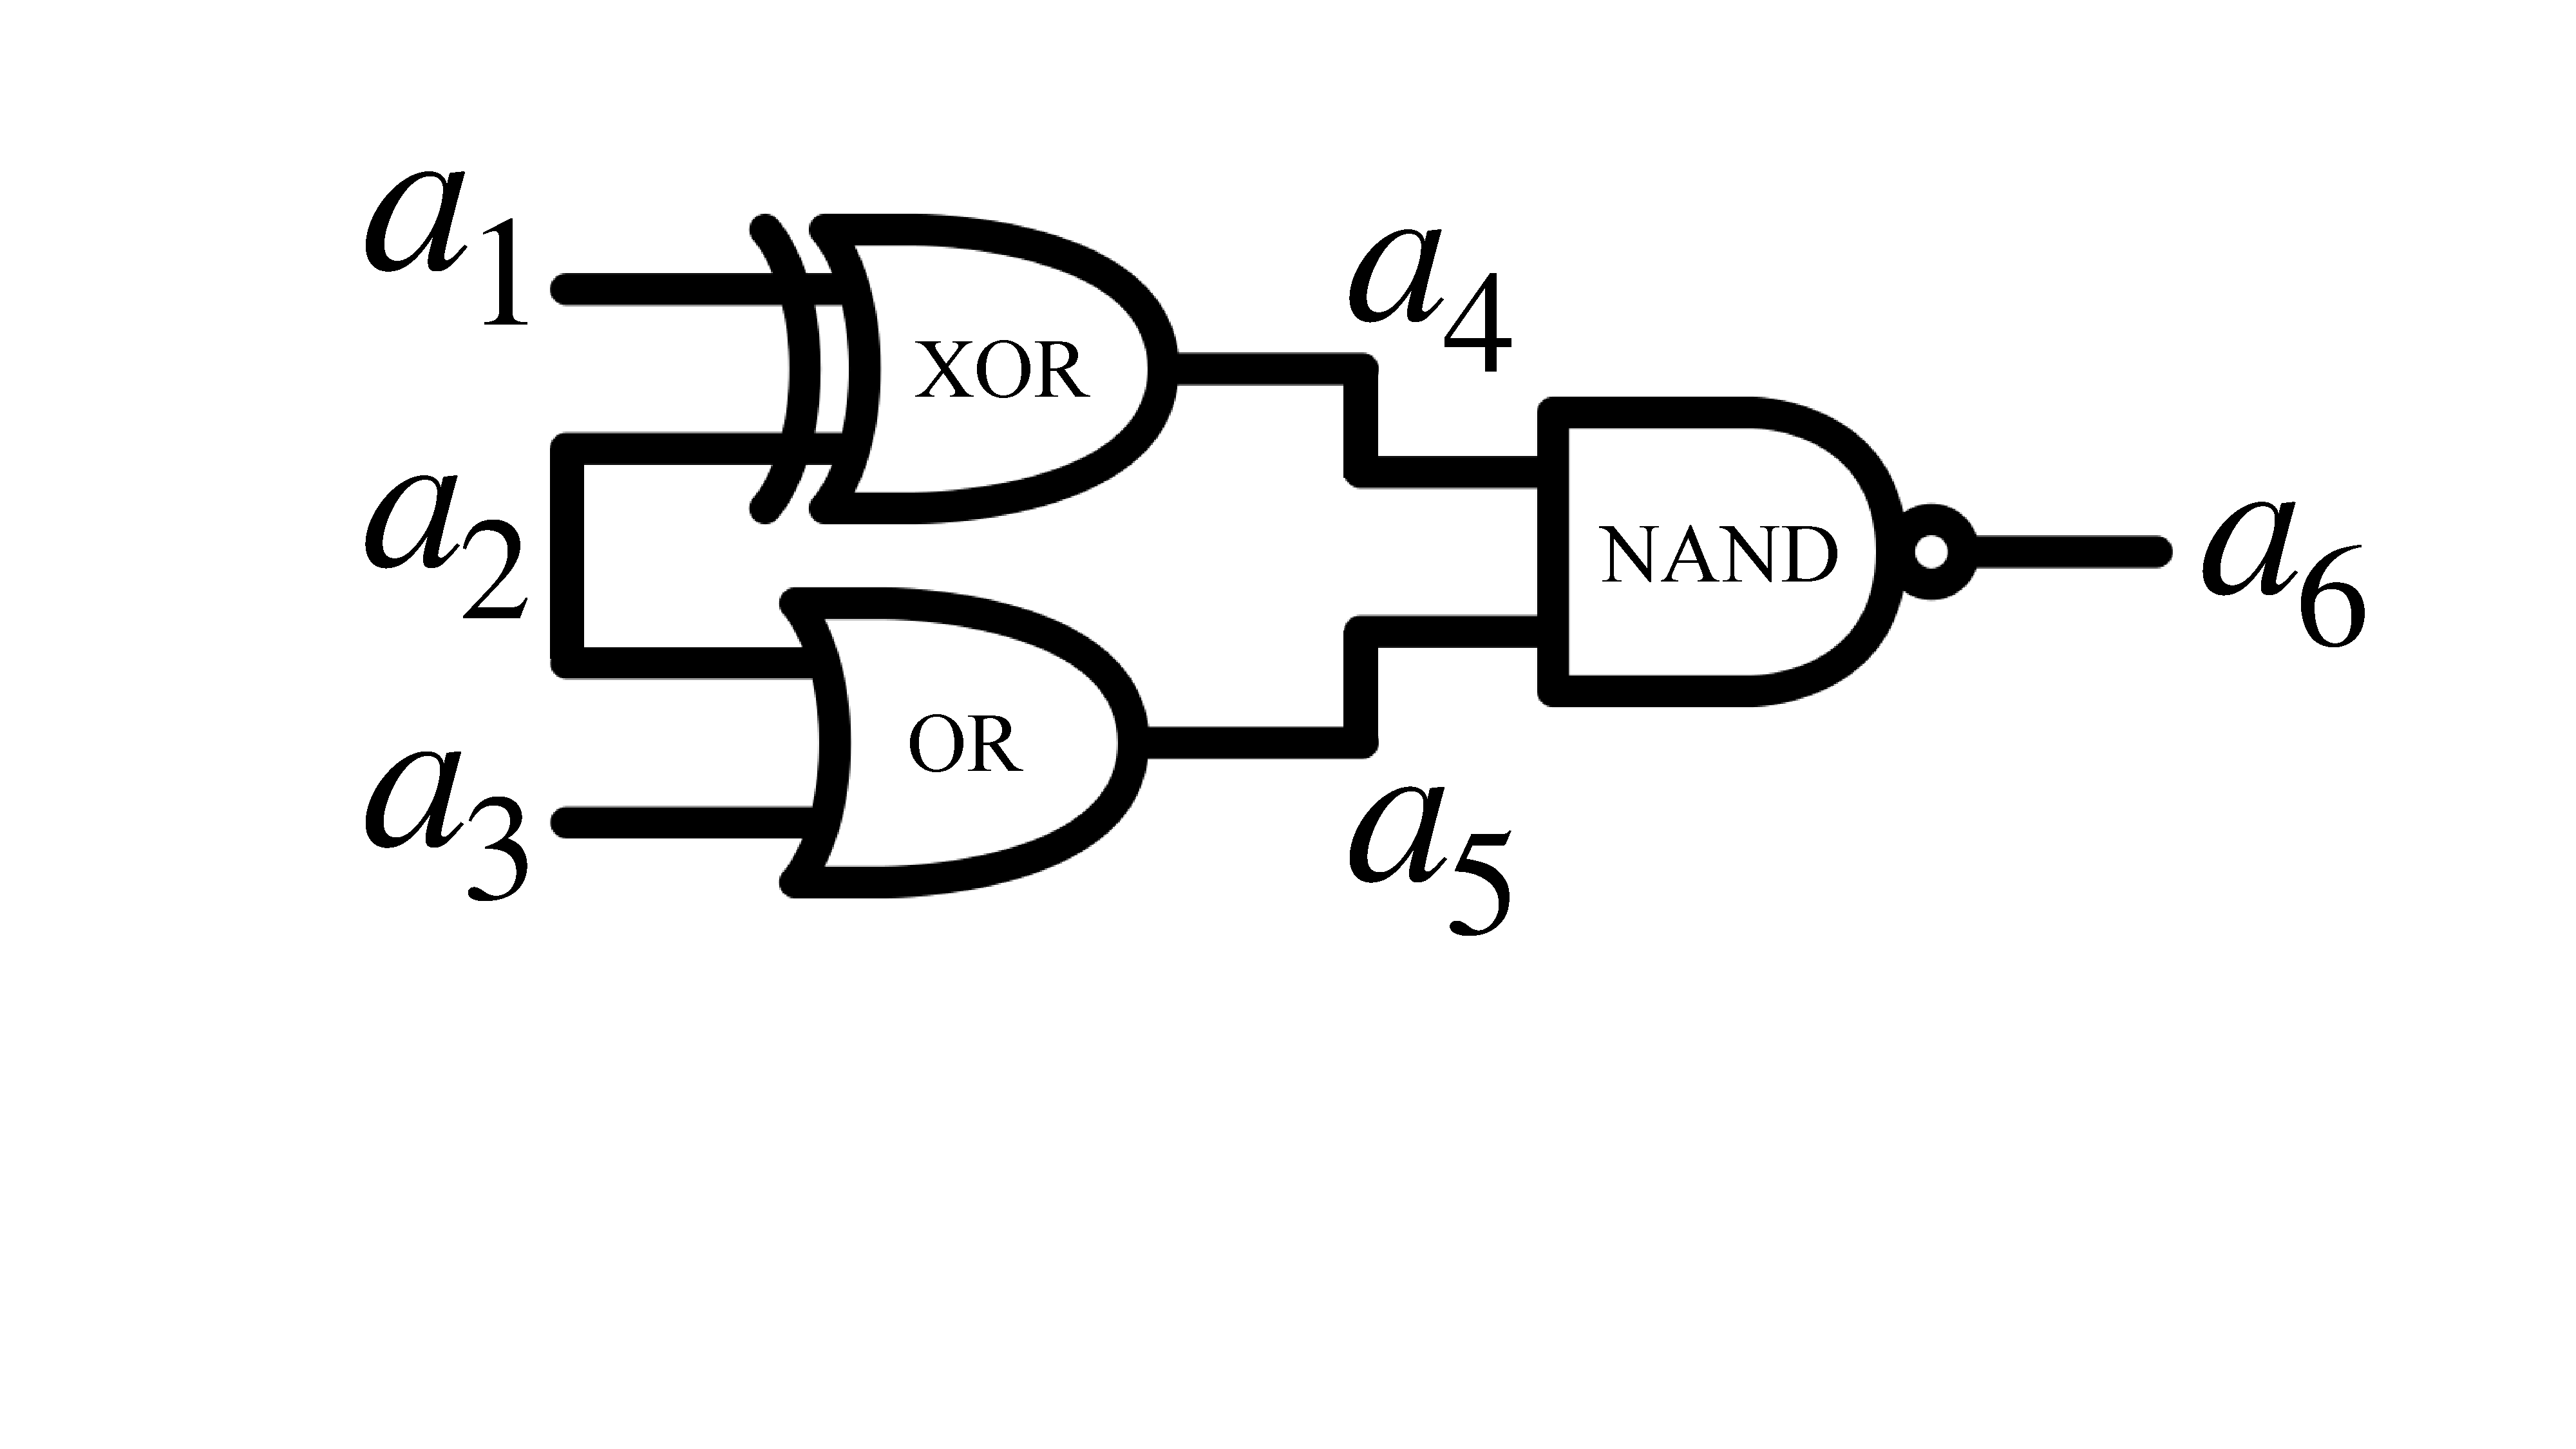
\includegraphics[width=0.4\textwidth]{figures/ssp.pdf}
  \caption{Boolean circuit example for SSP transformation \label{fig:ssp}} 
\end{figure}

First, we formalize the constraints for each gate type. For an XOR gate, the output $a_4$ of inputs $a_1, a_2$ must satisfy $a_1 + a_2 + a_4 \in \{0, 2\}$. For an OR gate, the output $a_5$ of inputs $a_2, a_3$ must satisfy $(1-a_2) + (1-a_3) - 2(1-a_5) \in \{0, 1\}$. For a NAND gate, the output $a_6$ of inputs $a_4, a_5$ must satisfy $a_4 + a_5 - 2(1-a_6) \in \{0, 1\}$.

For the circuit to be satisfiable, all gate constraints must be satisfied, the output constraint $3(1 - a_6) \in \{0, 2\}$ must hold, and all boolean value constraints $a_i \in \{0, 1\}$ for all $i \in \{1,\ldots,6\}$ must be met. To standardize these constraints, we multiply all constraints involving $\{0, 1\}$ by 2 to normalize ranges and combine constraints into a matrix form for $a_1,\ldots,a_6$. Finally, we seek to unify the constraints into a larger matrix that encompasses all the constraints in the whole circuit, where each column represents a single boolean algebra constraint. The resulting constraint matrix $M$ is below, with columns representing the XOR, OR, NAND, and output constraints, respectively:

\[ \begin{pmatrix}
1 & 0 & 0 & 0 & 2 & 0 & 0 & 0 & 0 & 0 \\
1 & -2 & 0 & 0 & 0 & 2 & 0 & 0 & 0 & 0 \\
0 & -2 & 0 & 0 & 0 & 0 & 2 & 0 & 0 & 0 \\
1 & 0 & 2 & 0 & 0 & 0 & 0 & 2 & 0 & 0 \\
0 & 4 & 2 & 0 & 0 & 0 & 0 & 0 & 2 & 0 \\
0 & 0 & 4 & -3 & 0 & 0 & 0 & 0 & 0 & 2
\end{pmatrix} \]

There is also a constant vector $c$ associated with these constraints:

\[ \vec{\delta} = [0 \; 0 \; -4 \; 3 \; | \; 0 \; 0 \; 0 \; 0 \; 0 \; 0] \]

All constraints must evaluate to elements in $\{0, 2\}^{10}$. 

\paragraph{Generalizing to Arbitrary Circuits.}

Let's now see how we can transform any arbitrary boolean circuit into a Square Span Program. Consider a circuit with $m$ wires and $n$ gates. Our first task is to construct a matrix that captures all the constraints of our circuit. For each gate $k$ in our circuit, we create a column vector $\vec{v_k} = (v_{1k}, v_{2k}, \ldots, v_{mk})^T$ that encodes the gate's constraints. These constraints ensure the gate operates correctly—just as we saw with our XOR, OR, and NAND gates in the previous example.

After encoding all $n$ gates, we add a special column for the output constraint, which takes the form $(0,\ldots,0,-3)^T$. The $-3$ here is somewhat arbitrary; any field element different from 2 would work. We then augment our matrix with a diagonal matrix $D$ where each diagonal entry is 2. This diagonal matrix serves to enforce that all our variables are boolean, a crucial requirement for circuit satisfaction.

To complete our constraint system, we need a constant vector $\vec{\delta} = (\delta_1,\ldots,\delta_n,3,0,\ldots,0)$ where each $\delta_i$ represents the constant term for gate $i$. These constants are chosen from the set $\{0,2\}$, with the exception of the output constraint's constant which is 3.

Let's now see how we can transform any arbitrary boolean circuit into a Square Span Program. Consider a circuit with $m$ wires and $n$ gates. The complete constraint system can be written as:

\[ \begin{pmatrix} a_1 & a_2 & \cdots & a_m \end{pmatrix}
\begin{pmatrix}
v_{11} & v_{12} & \cdots & v_{1n} & 0 & 2 & 0 & \cdots & 0 \\
v_{21} & v_{22} & \cdots & v_{2n} & 0 & 0 & 2 & \cdots & 0 \\
v_{31} & v_{32} & \cdots & v_{3n} & 0 & 0 & 0 & \ddots & 0 \\
\vdots & \vdots & \ddots & \vdots & \vdots & \vdots & \vdots & \ddots & \vdots \\
v_{m1} & v_{m2} & \cdots & v_{mn} & -3 & 0 & 0 & \cdots & 2
\end{pmatrix} + \begin{pmatrix} \delta_1 & \delta_2 & \cdots & \delta_n & 3 & 0 & \cdots & 0 \end{pmatrix} \]

where $(a_1,\ldots,a_m)$ are the wire values (variables we solve for), the first $n$ columns $(v_{ij})$ represent the gate constraints, column $n+1$ is the output constraint $(0,\ldots,0,-3)^T$, the next $m$ columns form the diagonal matrix $D$ with $2$'s on the diagonal, and the constant vector $(\delta_1,\ldots,\delta_m)$ contains $\delta_i \in \{0,2\}$ for $i \leq n$ (gate constraints), $\delta_{n+1} = 3$ (output constraint), and $\delta_i = 0$ for $i > n+1$ (boolean constraints).

Next, we convert these discrete constraints into a polynomial system. We choose distinct field elements $x_1,\ldots,x_d$ (where $d$ is our total number of constraints) and use polynomial interpolation to create our SSP. For each row $i$ of our matrix, we construct a polynomial $v_i(x)$ that evaluates to the $(i,j)$ entry when evaluated at point $x_j$. Similarly, we create a polynomial $v_0(x)$ that interpolates our constant vector $\vec{\delta}$.

The target polynomial $t(x)$ is defined as the product of all linear terms:

\[ t(x) = \prod_{j=1}^d (x-x_j) \]

This polynomial is crucial because it ``zeros out'' exactly at our constraint points. The beauty of this construction is that it transforms our circuit satisfaction problem into an elegant polynomial divisibility question: the circuit is satisfiable if and only if there exist values $(a_1,\ldots,a_m)$ such that:

\[ \left(v_0(x) + \sum_{i=1}^m a_i v_i(x)\right)^2 - 1 = h(x)t(x) \]

for some polynomial $h(x)$.

After converting to a polynomial system, our constraint matrix becomes:

\[ \begin{pmatrix} 
a_1 \\ 
a_2 \\ 
\vdots \\ 
a_m 
\end{pmatrix}^T
\begin{pmatrix}
v_1(x_1) & v_1(x_2) & \cdots & v_1(x_n) & v_1(x_{n+1}) & v_1(x_{n+2}) & 0 & \cdots & 0 \\
v_2(x_1) & v_2(x_2) & \cdots & v_2(x_n) & v_2(x_{n+1}) & 0 & v_2(x_{n+2}) & \cdots & 0 \\
v_3(x_1) & v_3(x_2) & \cdots & v_3(x_n) & v_3(x_{n+1}) & 0 & 0 & \ddots & 0 \\
\vdots & \vdots & \ddots & \vdots & \vdots & \vdots & \vdots & \ddots & \vdots \\
v_m(x_1) & v_m(x_2) & \cdots & v_m(x_n) & v_m(x_{n+1}) & 0 & v_m(x_{n+2}) & \cdots & v_m(x_d)
\end{pmatrix} + 
\begin{pmatrix} v_0(x_1) \\ v_0(x_2) \\ \vdots \\ v_0(x_n) \\ v_0(x_{n+1}) \\ v_0(x_{n+2}) \\ 0 \\ \vdots \\ 0 \end{pmatrix}^T \]

where:
\begin{itemize}
    \item Each $v_i(x_j)$ evaluates to the corresponding matrix entry at point $x_j$
    \item The diagonal entries evaluate to 2 at their respective points
    \item The output constraint column evaluates to $(0,\ldots,0,-3)$ at point $x_{n+1}$
    \item $v_0(x)$ interpolates the constant vector $(\delta_1,\ldots,\delta_n,3,0,\ldots,0)$
\end{itemize}

For any boolean circuit $C$, we can construct an SSP instance $(v_0(x),\ldots,v_m(x),t(x))$ such that $C(x_1,\ldots,x_\ell) = 1$ if and only if there exist values $(a_{\ell+1},\ldots,a_m)$ making the above polynomial division possible.

The correctness of this transformation follows from our construction: each gate's constraints are captured at distinct evaluation points, the boolean nature of our variables is enforced by the diagonal matrix, and the polynomial division condition.




Now, for notational convenience, we define $v_0'(x) = v_0(x) - 1$. 

At each evaluation point $x_j$, our circuit constraints require:
\[ \left(\sum_{i=1}^m a_i v_i(x_j) + v_0'(x_j)\right)^2 = 1 \]

This set of point-wise constraints can be unified into a single polynomial constraint:
\[ \left(\sum_{i=1}^m a_i v_i(x) + v_0'(x)\right)^2 - 1 \equiv 0 \pmod{t(x)} \]

where $t(x) = \prod_{j=1}^d (x - x_j)$ is our target polynomial.

Equivalently, there must exist some polynomial $h(x)$ such that:
\[ \left(\sum_{i=1}^m a_i v_i(x) + v_0'(x)\right)^2 - 1 = h(x)t(x) \]

This is precisely the SSP satisfiability condition. Thus, we have shown that circuit satisfiability is equivalent to the existence of coefficients $a_i$ that satisfy this polynomial divisibility condition.

\subsection{From SSPs to SNARKs}

We'll use bilinear groups to construct our SNARK. Our construction begins with a bilinear group setup:
\[ (\mathbb{F}_p, G_1, G_2, G_T, e, g_1, g_2) \]

The common reference string (CRS) forms the foundation of our construction. It consists of powers of a secret value $\tau$:
\[ \text{CRS} = (bg, g_1^\tau, g_1^{\tau^2}, \dots, g_1^{\tau^d}, g_2^\tau, g_2^{\tau^2}, \dots, g_2^{\tau^d}, g_1^{B v_{\ell + 1}(\tau)}, \dots, g_1^{B v_m(\tau)}, h_2, h_2^B) \]

The core idea of our construction leverages the pairing operation $e$ to verify polynomial equations in the exponent:
\[ e(g_1^{[v_0(x) + \sum_{i=1}^m a_i v_i(x)]}, g_2^{[v_0(x) + \sum_{i=1}^m a_i v_i(x)]}) = e(g_1^{h(x)}, g_2^{t(x)}) \cdot e(g_1, g_2) \]

In our protocol, we distinguish between two types of values:
\begin{itemize}
    \item Statement: $(a_1, \dots, a_\ell)$ - the public inputs
    \item Witness: $(a_{\ell+1}, \dots, a_m)$ - the private values
\end{itemize}

For proof generation, the prover computes four crucial group elements:
\begin{align*}
    \pi_1 &= g_1^{\sum_{i=\ell+1}^m a_i v_i(z)} \\
    \pi_2 &= g_2^{\sum_{i=\ell+1}^m a_i v_i(z)} \\
    \pi_3 &= g_1^{h(z)} \\
    \pi_4 &= g_1^{B\sum_{i=1}^m a_i v_i(z)}
\end{align*}

The verification process consists of two steps. First, the verifier computes intermediate values:
\begin{align*}
    \pi_1' &= g_1^{v_0(z) + \sum_{i=1}^\ell a_i v_i(z)} \cdot \pi_1 \\
    \pi_2' &= g_2^{v_0(z) + \sum_{i=1}^\ell a_i v_i(z)} \cdot \pi_2
\end{align*}

Then, the verifier performs three critical pairing checks:
\begin{align*}
    e(\pi_1', \pi_2') &= e(\pi_3, g_2^{t(z)}) \cdot e(g_1, g_2) \\
    e(\pi_1, g_2) &= e(g_1, \pi_2) \\
    e(\pi_1, h_2^B) &= e(\pi_4, h_2)
\end{align*}

These pairing equations serve distinct purposes in ensuring the proof's validity. The first check confirms that the SSP is satisfied by verifying the polynomial equation in the exponent. The second check ensures consistency between the prover's elements in groups $G_1$ and $G_2$. The final check prevents malformed group elements by verifying they were properly constructed using the CRS values.

Due to the non-interactive nature of our protocol, we cannot rely on black-box extraction for our security proofs. Instead, we require a non-black-box extractor with access to the prover's code, which is acceptable within our security model.

\subsection{Soundness}

The soundness guarantees of SNARKs, including our SSP SNARK construction, differ from traditional cryptographic protocols. They necessarily rely on non-falsifiable assumptions or the random oracle model (ROM).

Non-falsifiable assumptions represent a unique class of cryptographic assumptions. Informally, given $(g, g^\alpha)$, these assumptions state that no adversary can output a pair $(g^x, (g^x)^\alpha)$ without actually ``knowing'' the exponent $x$. The term ``non-falsifiable'' stems from the fact that these assumptions make claims about what an adversary must know, rather than just what it can or cannot compute.

Our first attempt at formalizing soundness states that for every probabilistic polynomial-time (PPT) adversary $\mathcal{A}$, there exists a PPT extractor $E_\mathcal{A}$ such that:
\[ \Pr[(v_1, v_2) \gets \mathcal{A}(g, g^\alpha, z), x \gets E_\mathcal{A}(g, g^\alpha, z) : v_2 = v_1^\alpha \land v_1 \neq g^x] = negl(\lambda) \]

This probability involves three key components:
\begin{itemize}
    \item $z$ represents auxiliary information available to the adversary
    \item $\lambda$ denotes the security parameter
    \item $negl(\lambda)$ represents a negligible function
\end{itemize}

Recent research has revealed limitations in this initial formulation. Specifically, certain obfuscated programs, when provided as auxiliary input $z$, enable adversaries to produce valid pairs $(v_1, v_2)$ while preventing the extractor $E_\mathcal{A}$ from determining $x$ due to the complexity of reverse-engineering the obfuscated program.

To address these limitations, we've developed a more robust formulation for our SNARK construction. For all relations $R \in \mathcal{R}$, benign auxiliary information $z \in \mathcal{Z}$, and non-uniform adversaries $\mathcal{A}$, there exists a non-uniform PPT extractor $E_\mathcal{A}$ such that for all benign $z \in \mathcal{Z}$:
\[ \begin{aligned}
&\Pr[((v_1, v_2); c_0, \dots, c_d) \gets (\mathcal{A} \| E_\mathcal{A})(bg, g_1, g_2, \dots, g_2^{\tau^d}, z) : \\
&\quad e(v_1, g_2) = e(g_1, v_2) \land v_1 \neq g_1^{\sum_{i=0}^d c_i \tau^i}] = negl(\lambda)
\end{aligned} \]

This refined definition captures several crucial aspects: the adversary and extractor share access to the bilinear group setup and CRS, the extractor must produce coefficients $c_i$ explaining the adversary's output, the auxiliary information must be ``benign'' (excluding problematic cases like obfuscated programs), and the probability of adversarial success without the extractor finding a valid witness must be negligible.

While this non-falsifiable assumption is stronger than traditional cryptographic assumptions, it appears to be necessary for constructing efficient SNARKs using current techniques.
%\let\counterwithout\relax
\let\counterwithin\relax

\let\proof\relax
\let\endproof\relax
\let\example\relax
\let\endexample\relax

%% Tikz configuration
\usetikzlibrary{shapes.geometric, arrows}

% Change thanks markers to numbers
\makeatletter
\let\@fnsymbol\@arabic
\makeatother

%% LLNCS hyperref requirement
\renewcommand\UrlFont{\color{blue}\rmfamily}

%% Eurocrypt requirement
\pagestyle{plain}


%% Allow align environment to span multiple pages
\allowdisplaybreaks

%% Theorem Environments

% Bold optional theorem titles
\makeatletter
\def\th@definition{%
  \thm@notefont{}% same as heading font
  \normalfont % body font
}
\makeatother

% No italics
% \theoremstyle{definition}

% Rename environments
\newtheorem{assumption}{Assumption}
% \newtheorem{construction}{Construction}
\newtheorem{attention}{Remark}
\newtheorem{notation}{Notation}

% Algorithm counter to construction
\makeatletter 
\renewcommand\thealgorithm{\theconstruction.\arabic{algorithm}} 
\@addtoreset{algorithm}{construction}
\makeatother

%% Annotations
\newcommand\todo[1]{\textcolor{red}{TODO: #1}}
\definecolor{comment-color}{RGB}{68, 59, 141}
\renewcommand{\algorithmiccomment}[1]{\textcolor{comment-color}{// #1}}
\newcommand\blue[1]{\textcolor{blue}{#1}}
\newcommand{\mathhl}[1]{\colorbox{yellow}{$\displaystyle #1$}}



%% Diagram Macros

\newcommand{\rightarr}[1]{\sendmessageright{length=2.5cm, top=\colorbox{white}{$#1$}, topstyle={yshift=-9}}}
\newcommand{\leftarr}[1]{\sendmessageleft{length=2.5cm, top=\colorbox{white}{$#1$}, topstyle={yshift=-9}}}

\newcommand{\cfbox}[2]{
    \colorlet{currentcolor}{.}
    {\color{#1}
    \fbox{\color{currentcolor}#2}}
}

\newcommand{\En}{\mathcal{K}}
\newcommand{\Gn}{\mathcal{G}}
\newcommand{\Po}{\mathcal{P}}
\newcommand{\V}{\mathcal{V}}


\newcommand{\niksdef}[6]{
For all expected polynomial-time adversaries 
$\mathcal{P}^*$ 
there exists an expected polynomial-time extractor
$\mathcal{E}$ such that
    \[
    \Pr_{\mathsf{r}}
    \left[
      \begin{array}{l}
        #6
      \end{array}
      \middle\vert
      \begin{array}{l}
        % Generator
        \mathsf{pp} \gets \mathcal{G}(1^{\lambda}, N),\\ 
        % Adversarial Statement, Proof
        (#1, #2, #4) \gets \mathcal{P}^*(\mathsf{pp}, \mathsf{r}),\\
        % Key Generator
        (\pk, \vk) \gets \En(\pp, #1),\\
        % Precondition
        #5,\\
        % Extractor
        #3 \gets \mathcal{E}(\pp, \mathsf{r})
      \end{array}
    \right]
    \approx 
    1
    \]
    where $\mathsf{r}$ denotes an arbitrarily long random tape.
}


% \newcommand{\pp}{\mathsf{pp}}
% \newcommand{\pk}{\mathsf{pk}}
% \newcommand{\vk}{\mathsf{vk}}

% \newcommand{\R}{\mathcal{R}}

\newcommand{\FP}{F'}
\newcommand{\io}{\mathsf{x}}
\newcommand{\fu}{\mathsf{u}}
\newcommand{\fw}{\mathsf{w}}
\newcommand{\acc}{\mathsf{U}}
\newcommand{\aw}{\mathsf{W}}
\newcommand{\trivi}{\fu_{\bot}}
\newcommand{\trivw}{\fw_{\bot}}
\newcommand{\fold}{\mathsf{NIFS}}
\newcommand{\snark}{\mathsf{SNARK}}
\newcommand{\RIVC}{\R_{\mathsf{IVC}}}
\newcommand{\Str}{\mathsf{s}}
\newcommand{\com}{\mathsf{com}}

% \newcommand{\Gen}{\mathsf{Gen}}
\newcommand{\Commit}{\mathsf{Commit}}

% \newcommand{\negl}[1]{\mathsf{negl}(#1)}

\section{Recursive Proofs of Knowledge}

In this lecture, 
we discuss recursive zero-knowledge succinct non-interactive
arguments of knowledge (zkSNARKs).
%
We assume familiarity with zkSNARKs.

\subsection{Introduction}

% Zero-Knowledge Proofs
Succinct non-interactive arguments of knowledge are short certificates that attest to the correct execution of a computation without revealing any secret inputs. 
%
Today, 
zero-knowledge proofs are being used 
to secure \emph{billions} of dollars worth of assets~\cite{zerocash, stark}.
%
Zero-knowledge proofs 
enable a new class of secure applications 
with enhanced integrity and privacy guarantees
such as verifiable databases~\cite{zkvsql, vsql, accountablestorage, integridb},
private voting protocols~\cite{privatevoting},
anonymous credentials~\cite{cinderella, dacreds},
and
private cryptocurrencies~\cite{zerocash, pinocchiocoin, stark}.

% Proving a Function
More technically, 
SNARKs 
(for circuit-satisfiability)
allow a prover to demonstrate that it knows a secret witness $w$
such that for prescribed circuit $F$ and prescribed input and output pair $(x, y)$ that $F(x, w) = y$.
%
% Proving Recursion
However, today, we will be interested in
proving \emph{recursive} computation. 
Without loss of generality, we are interested in proving \emph{tail}
recursion,
that is, we want to prove
(unbounded) recursive applications 
of a function $F$.
Unbounded recursion
in general allows us to implement more complex programming patterns such as 
$\mathsf{for}$ and $\mathsf{while}$, 
which are not bounded ahead of time.
This allows us to prove stateful computations with dynamic control flow.
%% Use cases
In practice, 
proving recursion allows us to recursively prove blockchain updates, verifiable delay functions, and even a universal machine,
where each recursive step is a single cycle of a CPU.


% Naive Solution
Historically, 
the best known approach to design a proof system for recursive applications of a function $F$ 
was to unroll the entire execution $F \circ F \circ \cdots \circ F$ into a monolithic arithmetic circuit,
and then use a standard proof system with succinct proofs for circuit satisfiability.
%
Unfortunately,
this would necessarily mean that the prover's space complexity would scale with the \emph{entire trace} of the computation.
%
Moreover, 
in the setting of preprocessed arguments of knowledge
(where the prover and verifier would process the circuit into a succinct key to use for multiple inputs)
this fixed the recursion-depth ahead of time,
which often does not reflect practice.

% Recursive Solution Overview
The first breakthrough was due to Valiant~\cite{valiant} in 2012, 
who proposed incrementally verifiable computation (IVC),
which reflected the recursive structure of the computation
into the proof itself:
%
Given a succinct proof $\pi_{i}$ attesting to $i$ steps of computation,
the prover can write a succinct proof $\pi_{i + 1}$ that attests to $i + 1$ steps
by proving the correct execution of an arithmetic circuit 
that runs the latest step of computation,
and checks $\pi_i$ 
(using the proof system's verifier).
This avoids having to fix the recursion depth ahead of time,
while ensuring that the prover's space complexity only scales with a single step of execution.

Although undoubtedly elegant, 
Valiant's technique introduces a subtle issue:
Proofs of knowledge must satisfy a stronger notion of soundness 
known as \emph{knowledge-soundness}.
%
Essentially,
a proof system is considered knowledge-sound 
if, 
for any successful prover with some secret input to the computation, 
there exists a corresponding \emph{extractor} that,
with at most polynomial overhead,
can retrieve this secret input given access to the ``source code'' of the prover.
%
This extractor-based definition becomes problematic in the recursive setting:
Recursive proofs require \emph{recursive extraction} 
in which the extractor for step $i$ 
plays the successful prover for the extractor at step $i - 1$. 
This incurs a polynomial blowup in the extractor for each successive recursive step. 
In particular, 
this results in a final extractor that runs in exponential-time with respect to the recursion-depth, 
which disqualifies it as a valid extractor. 
%
To account for this issue, 
Valiant's original technique 
(and modern techniques) 
can only provably guarantee logarithmic-depth recursion in standard models.

\subsection{Preliminaries}

We operate in the \textit{preprocessing model}, which means that a trusted party will be responsible for generating a prover and verifier key.

% Definition
\begin{definition}
   [Incrementally Verifiable Computation]\label{def:ivc}
   An 
   incrementally verifiable computation (IVC)  
   scheme is defined by
   PPT algorithms 
   $(\mathcal{G}, \mathcal{P}, \mathcal{V})$ 
   and deterministic $\En$
   denoting the generator, 
   the prover, 
   the verifier,
   and the encoder respectively,
   with the following interface
   \begin{itemize}
     \item $\mathcal{G}(1^\lambda, N) \to \pp$: 
     on input security parameter $\lambda$ and size bounds $N$, 
     samples public parameters $\pp$.
     \item $\En(\pp, F) \to (\pk, \vk)$: 
     on input public parameters $\pp$, 
     and polynomial-time function $F$,
     deterministically produces
     a prover key $\pk$ 
     and a verifier key $\vk$.
     \item $\mathcal{P}(\pk, (i, z_0, z_{i}), \omega_{i}, \pi_{i}) \to \pi_{i+1}$: 
     on input a prover key $\pk$, 
     a counter $i$, 
     an initial input $z_0$, 
     a claimed output after $i$ iterations $z_i$,
     a non-deterministic advice $\omega_i$,
     and an IVC proof $\pi_i$ attesting to $z_i$,
     produces a new proof $\pi_{i + 1}$ attesting to $z_{i + 1} = F(z_{i}, \omega_{i})$.
     \item $\mathcal{V}(\vk, (i, z_0, z_{i}), \pi_{i}) \to \{0, 1\}$: 
     on input a verifier key $\vk$,
     a counter $i$,
     an initial input $z_0$, 
     a claimed output after $i$ iterations $z_i$,
     and an IVC proof $\pi_i$ attesting to $z_i$,
     outputs $1$ if $\pi_i$ is accepting, and 
     $0$ otherwise.
   \end{itemize}
     An IVC scheme 
     $(\mathcal{G}, \En, \mathcal{P}, \mathcal{V})$
     satisfies the following requirements.
     \begin{enumerate}
     \item Perfect Completeness:    
     For any
     PPT adversary $\mathcal{A}$
     \begin{equation*}
     \Pr
     \left[
       \begin{array}{l}
         \mathcal{V}(\vk, (i + 1, z_0, z_{i + 1}), \pi_{i + 1}) = 1 
       \end{array}
       \middle\vert
       \begin{array}{l}
         \mathsf{pp} \gets \mathcal{G}(1^{\lambda}, N),\\
         (F, (i, z_0, z_i), (\omega_i, \pi_i)) \gets \mathcal{A}(\mathsf{pp}),\\
         (\pk, \vk) \gets \En(\pp, F),\\
         z_{i + 1} \gets F(z_{i}, \omega_{i}),\\
         \mathcal{V}(\vk, i, z_0, z_{i}, \pi_{i}) = 1,\\
         \pi_{i + 1} \gets \mathcal{P}(\pk, (i, z_0, z_i), (\omega_{i}, \pi_{i}))
       \end{array}
     \right] = 1
     \end{equation*}
     where $F$ is a polynomial-time computable function represented as an arithmetic circuit.
   \item Knowledge Soundness:
   Consider constant $n \in \mathbb{N}$.
   \niksdef
   % Structure
   {F} 
   % Statement
   {(z_0, z_i)}
   % Witness
   {(\omega_0, \ldots, \omega_{n - 1})}
   % Proof Format
   {\Pi}
   % Precondition
   {\mathcal{V}(\vk, (n, z_0, z), \Pi) = 1}
   % Postcondition
   {z_n = z \text{ where }\\ z_{i + 1} \gets F(z_i, \omega_i)\\
   \forall i \in \{0, \ldots, n - 1\}
   }
   Moreover, 
     $F$ is a polynomial-time computable function represented as an arithmetic circuit.
     \item Succinctness: 
     The size of an IVC proof $\pi$ is independent of the number of iterations $i$.
   \end{enumerate}
\end{definition}

\begin{definition}[Non-Interactive Argument of Knowledge]\label{def:nark}
   Consider a relation $\R$ over 
   public parameters, structure, instance, and witness tuples.
   A non-interactive argument of knowledge for $\R$ consists of PPT algorithms
   $(\Gn, \Po,\V)$ 
   and deterministic $\En$,
   denoting the generator, 
   the prover,    
   the verifier
   and the encoder respectively with the following interface.
   \begin{itemize}
       \item $\Gn(1^{\lambda}, N) \to \pp$: 
       On input security parameter $\lambda$,
       and length parameter $N$
       samples public parameters $\pp$.
       \item $\En(\pp, \Str) \to (\pk, \vk)$: 
       On input structure $\Str$, 
       representing common structure among instances,
       outputs the prover key $\pk$ and verifier key $\vk$.
       \item $\Po(\pk, u, w) \to \pi$: On input instance $u$ and
         witness $w$, outputs a proof $\pi$ proving that $(\pp, \Str, u, w) \in \R$.
       \item $\V(\vk, u, \pi) \to \{0, 1\}$: 
       Checks instance $u$ 
       given proof $\pi$.
   \end{itemize}
   An argument of knowledge satisfies \textit{completeness} if for any PPT adversary $\mathcal{A}$,
   \begin{align*}
   \Pr
   \left[
       \begin{array}{l}
       \V(\vk, u, \pi) = 1
       \end{array}
       \middle\vert
       \begin{array}{l}
       \pp \gets \Gn(1^{\lambda}, N),\\
       (\Str,(u, w)) \gets \mathcal{A}(\pp),\\
       (\pp, \Str, u, w) \in \R,\\
       (\pk, \vk) \gets \En(\pp, \Str),\\
       \pi \gets \Po(\pk, u, w)
       \end{array}
       \right]
   = 1.
   \end{align*}
   An argument of knowledge satisfies \textit{knowledge soundness} if for all PPT adversaries $\Po^*$ there exists a PPT extractor $\mathcal{E}$ such that for all randomness $\mathsf{r}$
   \[
   \Pr
   \left[
       \begin{array}{l}
       (\pp, \Str, u, w) \in \R
       \end{array}
       \middle\vert
       \begin{array}{l}
       \pp \gets \Gn(1^{\lambda}, N),\\
       (\Str,u,\pi) \gets \Po^*(\pp, \mathsf{r}),\\
       (\pk, \vk) \gets \En(\pp, \Str),\\
       \V(\vk, u, \pi) = 1,\\
       w \gets \mathcal{E}(\pp, \mathsf{r})
       \end{array}
       \right]
   \approx 1.
   \]
\end{definition}

\begin{definition}[Succinctness]
   A non-interactive argument system is succinct if the size of the proof $\pi$
   is polylogarithmic in the size of the witness $w$.
\end{definition}

\begin{definition}[Commitment Scheme]\label{def:commitment}
   A commitment scheme is defined by polynomial-time algorithm
   $\Gen : \mathbb{N}^2 \to P$
   that produces public parameters given the security parameter and size parameter, 
   a deterministic polynomial-time algorithm
   $\Commit : P \times M \times R \to C$
   that produces a commitment in $C$ given a public parameters, message, and randomness tuple
   such that 
   binding holds.
   That is, 
   for any $\mathsf{PPT}$ adversary $\mathcal{A}$,
   given
   $\pp \gets \Gen(\lambda, n)$,
   and given $((m_1, r_1), (m_2, r_2)) \gets \mathcal{A}(\pp)$
   we have that
   \[
       \Pr[(m_1, r_1) \neq (m_2, r_2) \land \Commit(\pp, m_1, r_1) = \Commit(\pp, m_2, r_2)] \approx 0.
   \]
   %
   The commitment scheme is deterministic if $\Commit$ does not use its randomness. 
 \end{definition}

 \begin{definition}[Circuit Satisfiability]
   We define the circuit satisfiability relation $\mathsf{CSAT}$
   over structure, instance, witness tuples
   as follows.
   \begin{equation*}
     \mathsf{CSAT}
     = 
     \left\{
     \begin{array}{l}
         % Statment, Witness
         (C, (x, y), w)
     \end{array}
     \middle\vert
     \begin{array}{l}
         C(x, w) = y
     \end{array}
     \right\}.
   \end{equation*}  
 \end{definition}

\subsection{Construction}

% Formal Construction

\begin{construction}[Incrementally Verifiable Computation]\label{cons:ivc}
   Given a 
   a succinct commitment scheme
   $(\Gen, \Commit)$
   and a
   succinct non-interactive argument of knowledge 
   $\snark$ for circuit-satisfiability
   we construct an IVC scheme as follows.
   
   %% Function F  
   Consider an arithmetic circuit $F$ 
   that takes non-deterministic input
   We begin by defining an augmented circuit
   $\FP$
   as follows,
   where all input arguments are taken as non-deterministic advice.
   %
   \begin{mdframed}[nobreak=true]
     \noindent \underline{$\FP(\io_i, \omega_i, \pi_i)$}:
     \begin{enumerate}
       \item Parse $(\vk_\snark, i, z_0, z_i) \gets \io_i$.
       \item  If $i = 0$:
       \begin{enumerate}
         \item Check that $z_0 = z_i$.
         \label{ivc:fp:base}
       \end{enumerate}
       \item Otherwise:
       \begin{enumerate} 
         \item Check that $\snark.\V(\vk_\snark, \io_i, \pi_i) = 1$.
         \label{ivc:fp:check:general}
       \end{enumerate}
       \item Output $\io_{i + 1} \gets (\vk_{\snark}, i + 1, z_0, F(z_i, \omega_i))$.
       \label{ivc:fp:output}
     \end{enumerate}  
   \end{mdframed} 
   %
   %
   Given the augmented circuit $\FP$,
   we define $(\Gn, \En, \Po, \V)$ as follows.
   \begin{mdframed}[nobreak=true]
     \underline{$\Gn(\lambda, N)$}:
     \begin{enumerate}
       \item Output $\pp \gets \snark.\mathcal{G}({\lambda}, N)$.
     \end{enumerate}
   \end{mdframed}
   %
   \begin{mdframed}[nobreak=true]
     \underline{$\En(\pp, F)$}:
     \begin{enumerate}
       
       \item Compute 
       $(\pk_\snark, \vk_\snark) \gets \snark.\En(\pp, \FP)$.
       \item Output $\pk \gets (\FP, \pk_\snark, \vk_\snark)$ and $\vk \gets \vk_\snark$.
     \end{enumerate}
   \end{mdframed}
   \begin{mdframed}[nobreak=true]
     \underline{$\Po(\pk, (i, z_0, z_i), (\omega_i, \pi_i))$}:
     \begin{enumerate} 
       \item Parse $(\FP, \pk_\snark, \vk_\snark) \gets \pk$.
       \item Compute
       $\io_{i + 1} \gets \FP(\vk_{\snark},
       (i, z_0, z_i), \omega_i, \pi_i)$.
       \item Let $\io_i \gets (\vk_{\snark}, i, z_0, z_i)$
       \label{ivc:prover:io}
       \item Output
       $
       \pi_{i + 1} \gets \snark.\Po(\pk_\snark, (\bot, \io_{i + 1}), (\io_i
       , \omega_i, \pi_i))
       $.
       \label{ivc:prover:proof}
     \end{enumerate} 
   \end{mdframed}
   %
   \begin{mdframed}[nobreak=true]
     \underline{$\V(\vk, (i, z_0, z_i), \pi_i)$}:
     \begin{enumerate}
       \item If $i = 0$: Check that $z_i = z_0$.
       \label{ivc:verifier:base}
       \item Otherwise:
       \begin{enumerate}
         \item Parse $\vk_{\snark} \gets \vk$.
         \item Let $\io_i \gets (\vk_\snark, i, z_0, z_i)$.
         \label{ivc:v:check:first}
         \item Check that
         $\snark.\V(\vk_\snark, (\bot, \io_i), \pi_i) = 1$.
         \label{ivc:v:check:second}
       \end{enumerate}
       
     \end{enumerate}
   \end{mdframed}
 \end{construction}

\begin{lemma}[Completeness]
 Construction~\ref{cons:ivc}
 is complete.
\end{lemma}
\newcommand{\proof}{\noindent{\bf Proof. }} %% To begin a proof write \proof

\begin{proof}
   % Adversary
 Consider arbitrary PPT adversary $\mathcal{A}$.
 % public parameters
 Suppose $\pp \gets \Gen(1^{\lambda}, N)$.
 % Structure, Instance, Witness
 Suppose that
 \[
 (F, (z_0, z_i, i), \pi_i) \gets \mathcal{A}(\pp).
 \]
 % Prover Key, Verifier Key
 Suppose that for
   $(\pk, \vk) \gets \En(\pp, F)$
 % Precondition
 we have that
 \begin{align}\label{ivc:completeness:precondition:verifier}
   \V(\vk, (z_0, z_{i}, i), \pi_{i}) = 1.
 \end{align}
 % Postcondition
 Then,
 given
 \begin{align*}
   z_{i + 1} \gets F(z_{i}, \omega_{i})
 \end{align*}
 and 
 \begin{align*}
   \pi_{i + 1} \gets \Po(\pk, (z_0, z_i, i), (\omega_i, \pi_i))
 \end{align*}
 we must show that
 \begin{align}\label{ivc:completeness:postcondition}
   \V(\vk, (z_0, z_{i+1}, N), \pi_{i + 1}) = 1
 \end{align}
 with probability $1$.
 %
 
 % Case i = 0
 Indeed, 
 consider the base case where $i = 0$.
 %
 Then, 
 by Precondition~\ref{ivc:completeness:precondition:verifier},
 by the verifier's check in the base case 
 (Step~\ref{ivc:verifier:base})
 we have that $z_0 = z_i$.
 %
 Therefore,
 $\Po$ can successfully compute $\io_{i + 1}$ 
 (Step~\ref{ivc:prover:io}),
 because the base case check of $\FP$ 
 (Step~\ref{ivc:fp:base}) passes.
 %
 Then,
 by construction of $\FP$
 (Step~\ref{ivc:fp:output})
 we have that 
 \[
   \io_{i + 1} = (\vk_{\snark}, i + 1, z_0, F(z_i, \omega_i))
 \]
 Moreover,
 by the completeness
 of $\snark$,
 we have that $\pi_{i + 1}$ generated by $\Po$ 
 (Step~\ref{ivc:prover:proof})
 is indeed satisfying.
 %
 Therefore, 
 both the checks of $\V$ in Steps~\ref{ivc:v:check:first} and~\ref{ivc:v:check:second}
 are passing.
 %
 As such,
 we have that postcondition~\ref{ivc:completeness:postcondition}
 holds.
 
 
 % Case i \geq 1
 Suppose instead that $i \geq 1$.
 %
 by Precondition~\ref{ivc:completeness:precondition:verifier},
 by the verifier's check in the general case 
 we have that
 \begin{align*}
   \snark.\V(\vk_\snark, (\bot, \io_i), \pi_i) = 1
 \end{align*}
 for $\io_i = (\vk_\snark, i, z_0, z_i)$.
 %
 Then,
 $\Po$ can successfully compute $\io_{i + 1}$ 
 (Step~\ref{ivc:prover:io}),
 as the SNARK verifier check in $\FP$
 (Step~\ref{ivc:fp:check:general})
 holds.
 %
 %
 Once again,
 by construction of $\FP$
 (Step~\ref{ivc:fp:output})
 we have that 
 \[
   \io_{i + 1} = (\vk_{\snark}, i + 1, z_0, F(z_i, \omega_i))
 \]
 Moreover,
 by the completeness
 of $\snark$,
 we have that $\pi_{i + 1}$ generated by $\Po$ 
 (Step~\ref{ivc:prover:proof})
 is indeed satisfying.
 %
 Therefore, 
 both the checks of $\V$ in Steps~\ref{ivc:v:check:first} and~\ref{ivc:v:check:second}
 are passing.
 %
 As such,
 we have that postcondition~\ref{ivc:completeness:postcondition}
 holds.
\end{proof}

\begin{lemma}[Knowledge-Soundness]
 Construction~\ref{cons:ivc}
 is knowledge-sound.
\end{lemma}

% Proof for ivc knowledge soundness

\begin{proof}
   % Premise
   Let $n$ be a global constant.
   %
   Consider a deterministic expected polynomial-time adversary $\Po^*$.
   %
   Let $\pp \gets \Gen(1^{\lambda}, N)$.
   %
   Suppose 
   on input $\pp$ and randomness $\mathsf{r}$,
   $\Po^*$
   outputs 
   polynomial-time function $F$,
   instance $(z_0, z)$,
   and IVC proof $\pi$. 
   %
   Let $(\pk, \vk) \gets \En(\pp, F)$.
   Suppose that
   % Precondition
   \begin{align*}
     \V(\vk, (z_0, z, n), \pi) = 1.
   \end{align*}
   % Postcondition
   We must construct an expected polynomial-time extractor $\mathcal{E}$
   that, 
   with input $(\pp, \mathsf{r})$,
   outputs $(\omega_0, \ldots, \omega_{n - 1})$ 
   such that by computing
   \begin{align*}
     z_{i + 1} \gets F(z_{i}, \omega_{i})
   \end{align*}
   we have that $z_n = z$ with probability 
   $1 - \negl{\lambda}$.
   
   % Overview
   We show inductively that we can construct an expected polynomial-time extractor $\mathcal{E}_i$ that outputs 
   $((z_i, \ldots, z_{n - 1}), (\omega_i, \ldots, \omega_{n - 1}), \pi_i)$ such that for all $j \in  \{i + 1, \ldots, n\}$,
   \begin{align*}
     z_j = F(z_{j - 1}, \omega_{j - 1})
   \end{align*}
   and 
   \begin{align}\label{eq:ih:2}
     \V(\vk, z_0, z_i, \pi_i) = 1
   \end{align}
   for $z_n = z$ with probability $1 - \negl{\lambda}$.
   %
   Then, 
   because when $i = 0$,
   $\V$ checks that $z_0 = z_i$ 
   the values $(\omega_0, \ldots, \omega_{n - 1})$ 
   retrieved by $\mathcal{E} = \mathcal{E}_0$
   are such that computing  
   $z_{i + 1} = F(z_i, \omega_i)$ for all $i \geq 1$ gives $z_n = z$.
   
   At a high level,
   to construct an extractor $\mathcal{E}_{i - 1}$,
   we first assume the existence of $\mathcal{E}_i$ that satisfies the inductive hypothesis. 
   We then use $\mathcal{E}_i$ to construct an adversary 
   for the underlying succinct non-interactive argument, which we denote as $\widetilde{\Po}_{i - 1}$.
   This in turn guarantees an extractor for the underlying non-interactive argument,
   which we denote as $\widetilde{\mathcal{E}}_{i - 1}$. 
   We then use $\widetilde{\mathcal{E}}_{i - 1}$ to construct $\mathcal{E}_{i - 1}$ that satisfies the inductive hypothesis.
   
   
   % Base case
   In the base case,
   let $\mathcal{E}_n(\pp, \mathsf{r})$ 
   output 
   $(\bot, \bot, \pi_n)$ 
   where $\pi_n$ is the output of 
   $\Po^*(\pp, \mathsf{r})$.
   By the premise,
   we have that $\pi_n$ is satisfying.
   As such,
   $\mathcal{E}_n$ succeeds with probability $1 - \negl{\lambda}$ in expected polynomial-time.
   
   % Inductive Step
   For $i \geq 1$, 
   suppose we can construct an expected polynomial-time extractor 
   $\mathcal{E}_i$ 
   that outputs
   $((z_i, \ldots, z_{n - 1}), (\omega_i, \ldots, \omega_{n - 1}))$, 
   and $\pi_i$ 
   that satisfies the inductive hypothesis.
   % Construct SNARK prover
   To construct an extractor $\mathcal{E}_{i - 1}$, 
   we first construct an adversary $\widetilde{\Po}_{i - 1}$
   for the underlying SNARK as follows.
   %
   %
   %
   \begin{mdframed}[nobreak=true]
     \noindent \underline{$\widetilde{\Po}_{i - 1}(\pp, \mathsf{r})$}: 
     \begin{enumerate}
       \item Let $(F, z_0) \gets \Po^*(\pp, \mathsf{r})$
       \item Let $((z_i, \ldots, z_{n - 1}), (\omega_i, \ldots, \omega_{n -
       1}), \pi_i) \gets \mathcal{E}_i(\pp, \mathsf{r})$.
       \item Let $\vk_{\snark} \gets \snark.\En(\pp, F)$.
       \item Let $\io_i \gets (\vk_\snark, (i, z_0, z_i))$.
       \item Output $(\FP, (\bot, \io_i), \pi_i)$.
     \end{enumerate}
   \end{mdframed}
   
   % SNARK prover success probability
   We now analyze the success probability of $\widetilde{\Po}_{i - 1}$. 
   By the inductive hypothesis,
   we have that 
   \[
   \V(\vk, z_0, z_i, \pi_i) = 1,
   \]
   where 
   $\pi_i \gets \mathcal{E}_i(\pp, \mathsf{r})$ 
   with probability 
   $1 - \negl{\lambda}$.
   Therefore, 
   by the the verifier's checks 
   we have that
   \[
   \snark.\V(\vk_\snark, (\bot, \io_i), \pi_i) = 1
   \]
   for $\io_i = (\vk_\snark, (i, z_0, z_i))$
   and $\vk_\snark \gets \snark.\En(\pp, \FP)$.
   Therefore,
   $\widetilde{\Po}_{i - 1}$
   succeeds in producing a satisfying proof $\pi_i$
   for structure $\FP$ and instance $\io_i$
   with probability $1 - \negl{\lambda}$.
 
   
   % Corresponding SNARK extractor
   Then,
   by the knowledge soundness of $\snark$
   there exists an 
   expected-polynomial-time
   extractor $\widetilde{\mathcal{E}}_{i - 1}$ that
   outputs 
   $(\io_{i - 1}, \omega_{i - 1}, \pi_{i - 1})$
   such that
   $\io_i = \FP(\io_{i - 1}, \omega_{i - 1}, \pi_{i - 1})$
   with probability $1 - \negl{\lambda}$.
   
   % Constructing E_{i - 1}
   Given $\widetilde{\mathcal{E}}_{i - 1}$, 
   we construct an expected polynomial time $\mathcal{E}_{i - 1}$ as follows.
 
 
   \begin{mdframed}[nobreak=true]
   \noindent \underline{$\mathcal{E}_{i - 1}(\pp, \mathsf{r})$}: 
   \begin{enumerate}
     \item Run $\widetilde{\Po}_{i - 1}(\pp, \mathsf{r})$
     to parse
     \[
     ((z_i, \ldots, z_{n - 1}), (\omega_i, \ldots, \omega_{n -
     1}), \pi_i)
     \]
     from its internal state.
     \item Compute $(\io_{i - 1}, \omega_{i - 1}, \pi_{i - 1}) \gets \widetilde{\mathcal{E}}_{i - 1}(\pp, \mathsf{r})$.
     \item Parse $(\vk_\snark, (i - 1, z_0, z_{i - 1})) \gets \io_{i - 1}$
     \item Output $((z_{i - 1}, \ldots, z_{n - 1}), (\omega_{i - 1}, \ldots, \omega_{n - 1}), \pi_{i - 1})$. 
   \end{enumerate}
 \end{mdframed}
 
  We now reason about the success probability of $\mathcal{E}_{i - 1}$.
   We first reason that the output $(z_{i - 1}, \ldots, z_{n - 1})$, and
   $(\omega_{i - 1}, \ldots, \omega_{n - 1})$ are valid.
   By the inductive hypothesis, 
   we already have that for all $j \in \{i + 1, \ldots, n\}$,
   \begin{align*}
     z_j = F(z_{j - 1}, \omega_{j - 1})
   \end{align*}
   with probability $1 - \negl{\lambda}$.
   Moreover,
   by the success probability of $\mathcal{E}_{i - 1}$,
   we have that
   \begin{align*}
     z_{i} = F(z_{i - 1}, \omega_{i - 1})
   \end{align*}
   and that
   \[
   \snark.\V(\vk_\snark, \io_{i - 1}, \pi_{i - 1}) = 1
   \]
   where $\io_{i - 1} = (\vk_\snark, (i - 1, z_0, z_i))$
   with probability $1 - \negl{\lambda}$.
   %
   Therefore we have that $\mathcal{E}_{i - 1}$
   succeeds with probability $1 - \negl{\lambda}$
   satisfying the inductive hypothesis.
 \end{proof} 
%\newcommand{\proofsketch}{\smallskip\noindent{\bf Proof sketch. }}
\algrenewcommand\algorithmicfunction{\textbf{Machine}}
\newcommand{\bits}{\set{0,1}}
\newcommand{\Ex}{\mathbb{E}}

\renewcommand{\O}{\ensuremath{\mathcal{O}}}
\newcommand{\To}{\rightarrow}
\newcommand{\e}{\epsilon}
\newcommand{\R}{\mathbb{R}}
\newcommand{\N}{\mathbb{N}}
\newcommand{\Z}{\mathbb{Z}}
\newcommand{\logAnd}{\wedge}

\newcommand{\indis}{\mathrel{\overset{\makebox[0pt]{\mbox{\normalfont\tiny c}}}{\approx}}}
\newcommand{\allindis}{\mathrel{\overset{\makebox[0pt]{\mbox{\normalfont\tiny p/s/c}}}{\approx}}}

\newcommand{\cclass}[1]{\mathsf{#1}}
\renewcommand{\P}{\cclass{P}}
\newcommand{\NP}{\cclass{NP}}
\newcommand{\Time}{\cclass{Time}}
\newcommand{\BPP}{\cclass{BPP}}
\newcommand{\Size}{\cclass{Size}}
\newcommand{\Ppoly}{\cclass{P_{/poly}}}
\newcommand{\CSAT}{\ensuremath{\mathsf{CSAT}}}
\newcommand{\SAT}{\ensuremath{\mathsf{3SAT}}}
\newcommand{\IS}{\mathsf{INDSET}}



\newcommand{\inp}{\mathsf{in}}
\newcommand{\outp}{\mathsf{out}}

\newcommand{\Param}{\kappa}
\newcommand{\Adv}{\mathsf{Adv}}
\newcommand{\Supp}{\mathsf{Supp}}


\newcommand{\PRG}{\mathsf{G}}
\renewcommand{\Enc}{\mathsf{Enc}}
\renewcommand{\Dec}{\mathsf{Dec}}
\renewcommand{\sk}{\mathsf{sk}}
\newcommand{\sfC}{\mathsf{C}}
\newcommand{\sfR}{\mathsf{R}}

\newcommand{\eqdef}{\stackrel{\text{\tiny def}}{=}}

\newcommand{\cF}{\mathcal{F}}

\newcommand{\angles}[1]{\langle #1 \rangle}
\newcommand{\iprod}[1]{\angles{#1}}

\newcommand{\Com}{\mathsf{Com}}


% Real vs. Ideal
\newcommand{\RealAdv}{\mathcal{A}}
\newcommand{\IdealAdv}{\mathcal{S}}
\newcommand{\RealVar}{\mathsf{Real}}
\newcommand{\IdealVar}{\mathsf{Ideal}}

% Participating parties
\newcommand{\PartyA}{P_1}
\newcommand{\PartyB}{P_2}
\newcommand{\InputA}{x_1}
\newcommand{\InputB}{x_2}


% Garbling Schemes
\newcommand{\Garble}{\mathsf{Garble}}
\newcommand{\Cir}{C}
\newcommand{\GCir}{\widetilde{C}}
\newcommand{\Lab}{\mathsf{lab}}

% Proof
\newcommand{\Sim}{\mathsf{Sim}}

% GMW

% Misc
\newcommand{\out}{\mathsf{out}}
\newcommand{\Assign}{:=}

\chapter{Secure Computation}

\section{Introduction}
Secure multiparty computation considers the problem of different parties
computing a joint function of their separate, private inputs without revealing
any extra information about these inputs than that is leaked by just the result
of the computation. This setting is well motivated, and captures many different
applications. Considering some of these applications will provide intuition
about how security should be defined for secure computation:
\begin{description}
  \item[Voting:] Electronic voting can be thought of as a multi party computation
	  between $n$ players: the voters. Their input is their choice $b \in \{0,1\}$
    (we restrict ourselves to the binary choice setting without loss of generality), and the function
    they wish to compute is the majority function.

    Now consider what happens when only one user votes: their input is trivially
    revealed as the output of the computation. What does privacy of inputs mean
    in this scenario?

  \item[Searchable Encryption:] Searchable encryption schemes allow clients
    to store their data with a server, and subsequently grant servers tokens
    to conduct specific searches. However, most schemes do not consider access
    pattern leakage. This leakage tells the server potentially valuable information
    about the underlying plaintext. How do we model all the different kinds
    information that is leaked?
\end{description}

From these examples we see that defining security is tricky, with lots of
potential edge cases to consider. We want to ensure that no party can learn
anything more from the secure computation protocol than it can from just its
input and the result of the computation. To formalize this, we adopt the
\textbf{real/ideal paradigm}.



\section{Real/Ideal Paradigm}
\paragraph{Notation.} 
Suppose there are $n$ parties, and party $P_i$ has access to some data $x_i$. They are trying to compute some function of their inputs $f(x_1, \dotsc, x_n)$. The goal is to do this securely: even if some parties are corrupted, no one should learn more than is strictly necessitated by the computation.

\paragraph{Real World.} In the real world, the $n$ parties execute a protocol $\Pi$
to compute the function $f$. This protocol can involve multiple rounds of
interaction. %Each party can additionally have some randomness.
The real world adversary $\RealAdv$ can corrupt arbitrarily many (but not all) parties.


\paragraph{Ideal World.} In the ideal world, an angel helps in the
computation of $f$:
each party sends their input to the angel and receives the output of the computation $f(x_1, \dotsc, x_n)$.
Here the ideal world adversary $\IdealAdv$ can again corrupt arbitrarily many (but not all) parties.

To model malicious adversaries, we need to modify the ideal world model as follows. 
Some parties are honest, and each honest party $P_i$ simply sends $x_i$ to the angel. The other parties are corrupted and are under control of the adversary $\IdealAdv$. The adversary chooses an input $x_i'$ for each corrupted party $P_i$ (where possibly $x_i' \neq x_i$) and that party then sends $x_i'$ to the angel. The angel computes a function $f$ of the values she receives (for example, if only party 1 is honest, then the angel computes $f(x_1, x_2', x_3', \dotsc, x_n')$) in order to obtain a tuple $(y_1, \dotsc, y_n)$. 
She then sends $y_i$ of corrupted parties to the adversary, who gets to decide whether or not honest parties will receive their response from the angel. The angel obliges. Each honest party $P_i$ then outputs $y_i$ if they receive $y_i$ from the angel and $\perp$ otherwise, and corrupted parties output whatever the adversary tells them to. 

 



\paragraph{Definition of Security.} 
A protocol $\Pi$ is secure against computationally bounded adversaries if for every PPT adversary $\RealAdv$ in the real world, there exists an PPT adversary $\IdealAdv$ in the ideal world such that for all tuples of bit strings $(x_1, \dotsc, x_n)$, we have
\[ \mathrm{Real}_{\Pi, \RealAdv}(x_1, \dotsc x_n) \stackrel{c}{\simeq} \mathrm{Ideal}_{F,\IdealAdv}(x_1, \dotsc, x_n) \]
where the left-hand side denotes the output distribution induced by $\Pi$ running with $\RealAdv$, and the right-hand side denotes the output distribution induced by running the ideal protocol $F$ with $\IdealAdv$. 
The ideal protocol is either the original one described for semi-honest adversaries, or the modified one described for malicious adversaries. 





%We require that the views of the parties
%in each of the scenarios be identical, i.e.\ that a real-world execution of the
%protocol $\Pi$ should not leak any information not leaked by the ideal-world
%execution. Hence, the parties can only learn what they can infer from their
%inputs and the output $f(\InputA, \InputB)$. More formally, assuming $\RealAdv$
%corrupts one party (say $\PartyA$, wlog), we define random variables
%$\RealVar_{\Pi, \RealAdv}(\InputA, \InputB) = \RealAdv(\InputA, r_1, \text{messages
%sent in } \Pi)$ and $\IdealVar_{F, \IdealAdv}(\InputA, \InputB) = \IdealAdv(\InputA,
%f(\InputA,\InputB))$.  These random variables represent the views of the
%adversary in each of the two settings. Our definition of security thus requires
%that
%
%\begin{equation*}
%\RealVar_{\Pi, \RealAdv}(\InputA, \InputB) \indis \IdealVar_{F, \IdealAdv}(x_1, x_2).
%\end{equation*}

\paragraph{Assumptions.} We have brushed over some details of the above setting.
Below we state these assumptions explicitly:
\begin{enumerate}
  \item \textbf{Communication channel:} We assume that the communication channel
    between the involved parties is completely insecure, i.e., it does not preserve
    the privacy of the messages. However, we assume that it is reliable, which means
    that the adversary can drop messages, but if a message is delivered, then
    the receiver knows the origin.

  \item \textbf{Corruption model:} We have different models of how and when the
    adversary can corrupt parties involved in the protocol:
    \begin{itemize}
      \item
        \emph{Static:} The adversary chooses which parties to corrupt before the
        protocol execution starts, and during the protocol, the malicious parties
        remain fixed.
      \item
        \emph{Adaptive:} The adversary can corrupt parties dynamically during
        the protocol execution, but the simulator can do the same.
      \item
        \emph{Mobile:} Parties corrupted by the adversary can be ``uncorrupted''
        at any time during the protocol execution at the adversary's discretion.
    \end{itemize}

  \item \textbf{Fairness:} The protocols we consider are not ``fair'', i.e.,
    the adversary can cause corrupted parties to abort arbitrarily. This can
    mean that one party does not get its share of the output of the computation.

  \item \textbf{Bounds on corruption:} In some scenarios, we place upper bounds
    on the number of parties that the adversary can corrupt.

  \item \textbf{Power of the adversary:} We consider primarily two types of
    adversaries:
    \begin{itemize}
      \item \emph{Semi-honest adversaries:} Corrupted parties follow the protocol
        execution $\Pi$ honestly, but attempt to learn as much information as they
        can from the protocol transcript.

      \item \emph{Malicious adversaries:} Corrupted parties can deviate arbitrarily
        from the protocol $\Pi$.
    \end{itemize}

  \item \textbf{Standalone vs.\ Multiple execution:} In some settings, protocols
    can be executed in isolation; only one instance of a particular protocol
    is ever executed at any given time. In other settings, many different protocols
    can be executed concurrently. This can compromise security.
\end{enumerate}







\section{Oblivious transfer}

\emph{Rabin's oblivious transfer} sets out to accomplish the following special task of two-party secure computation. The sender has a bit $s \in \{0,1\}$. She places the bit in a box. Then the box reveals the bit to the receiver with probability 1/2, and reveals $\perp$ to the receiver with probability 1/2. The sender cannot know whether the receiver received $s$ or $\perp$, and the receiver cannot have any information about $s$ if they receive $\perp$.

\subsection{1-out-of-2 oblivious transfer}
\emph{1-out-of-2 oblivious transfer} sets out to accomplish the following related task. The sender has two bits $s_0, s_1 \in \{0,1\}$ and the receiver has a bit $c \in \{0,1\}$. The sender places the pair $(s_0, s_1)$ into a box, and the receiver places $c$ into the same box. The box then reveals $s_c$ to the receiver, and reveals $\perp$ to the sender (in order to inform the sender that the receiver has placed his bit $c$ into the box and has been shown $s_c$). The sender cannot know which of her bits the receiver received, and the receiver cannot know anything about $s_{1-c}$.

\begin{lemma}
A system implementing 1-out-of-2 oblivious transfer can be used to implement Rabin's oblivious transfer.
\end{lemma}

\proof
The sender has a bit $s$. She randomly samples a bit $b \in \{0,1\}$ and $r \in \{0,1\}$, and the receiver randomly samples a bit $c \in \{0,1\}$. If $b = 0$, the sender defines $s_0 = s$ and $s_1 = r$, and otherwise, if $b = 1$, she defines $s_0 = r$ and $s_1 = s$. She then places the pair $(s_0, s_1)$ into the 1-out-of-2 oblivious transfer box. The receiver places his bit $c$ into the same box, and then the box reveals $s_c$ to him and $\perp$ to the sender. Notice that if $b = c$, then $s_c = s$, and otherwise $s_c = r$. Once $\perp$ is revealed to the sender, she sends $b$ to the receiver. The recieiver checks whether or not $b = c$. If $b = c$, then he knows that the bit revealed to him was $s$. Otherwise, he knows that the bit revealed to him was the nonsense bit $r$ and he regards it as $\perp$. \\

It is easy to see that this procedure satisfies the security requirements of Rabin's oblivious transfer protocol. Indeed, as we saw above, $s_c = s$ if and only if $b = c$, and since the sender knows $b$, we see that knowledge of whether or not the bit $s_c$ received by the receiver is equal to $s$ is equivalent to knowledge of $c$, and the security requirements of 1-out-of-2 oblivious transfer prevent the sender from knowing $c$. Also, if the receiver receives $r$ (or, equivalently, $\perp$), then knowledge of $s$ is knowledge of the bit that was not revealed to him by the box, which is again prevented by the security requirements of 1-out-of-2 oblivious transfer.  $\qed$

\begin{lemma}
A system implementing Rabin's oblivious transfer can be used to implement 1-out-of-2 oblivious transfer.
\end{lemma}

\proofsketch
The sender has two bits $s_0, s_1 \in \{0,1\}$ and the receiver has a single bit $c$. The sender randomly samples $3n$ random bits $x_1, \dotsc, x_{3n} \in \{0,1\}$. Each bit is placed into its own a Rabin oblivious transfer box. The $i$th box then reveals either $x_i$ or else $\perp$ to the receiver. Let 
\[ S := \{i \in \{1, \dotsc, 3n\} : \text{the receiver knows } x_i\}. \]
The receiver picks two sets $I_0, I_1 \subseteq \{1, \dotsc, 3n\}$ such that $\# I_0 = \# I_1 = n$, $I_c \subseteq S$ and $I_{1-c} \subseteq \{1, \dotsc, 3n\} \setminus S$. This is possible except with probability negligible in $n$. He then sends the pair $(I_0, I_1)$ to the sender. The sender then computes $t_j= \left(\bigoplus_{i \in I_j}x_i \right) \oplus s_j$ for both $j \in \{0,1\}$ and sends $(t_0, t_1)$ to the receiver. \\

Notice that the receiver can uncover $s_c$ from $t_c$ since he knows $x_i$ for all $i \in I_c$, but cannot uncover $s_{1-c}$. One can show that the security requirement of Rabin's oblivious transfer implies that this system satisfies the security requirement necessary for 1-out-of-2 oblivious transfer. $\qed$ \\

We will see below that length-preserving one-way trapdoor permutations can be used to realize 1-out-of-2 oblivious transfer. 

\begin{theorem}
The following protocol realizes 1-out-of-2 oblivious transfer in the presence of computationally bounded and semi-honest adversaries. 
\begin{enumerate}
\item The sender, who has two bits $s_0$ and $s_1$, samples a random length-preserving one-way trapdoor permutation $(f, f^{-1})$ and sends $f$ to the receiver.  Let $b(\cdot)$ be a hard-core bit for $f$.
\item The receiver, who has a bit $c$, randomly samples an $n$-bit string $x_c \in \{0,1\}^n$ and computes $y_c = f(x_c)$. He then samples another random $n$-bit string $y_{1-c} \in \{0,1\}^n$, and then sends $(y_0, y_1)$ to the sender.
\item The sender computes $x_0 := f^{-1}(y_0)$ and $x_1 := f^{-1}(y_1)$. She computes $b_0 := b(x_0) \oplus s_0$ and $b_1 := b(x_1) \oplus s_1$, and then sends the pair $(b_0, b_1)$ to the receiver.
\item The receiver knows $c$ and $x_c$, and can therefore compute $s_c = b_c \oplus b(x_c)$. 
\end{enumerate}
\end{theorem}
\proof
Correctness is clear from the protocol.	
For security, from the sender side, since $f$ is a length-preserving permutation, $(y_0, y_1)$ is statistically indistinguishable from two random strings, hence she can't learn anything about $c$.
From the receiver side, guessing $s_{1-c}$ correctly is equivalent to guessing the hard-core bit for $y_{1-c}$.
\qed


\subsection{1-out-of-4 oblivious transfer}
  We describe how to implement a 1-out-of-4 OT using 1-out-of-2 OT:\@
  \begin{enumerate}
    \item
      The sender, $\PartyA$ samples 5 random values $S_i \gets \bits, i \in \set{1,\dotsc, 5}$.
    \item
      $\PartyA$ computes
      \begin{align*}
        \alpha_0 &= S_0 \xor S_2 \xor m_0\\
        \alpha_1 &= S_0 \xor S_3 \xor m_1\\
        \alpha_2 &= S_1 \xor S_4 \xor m_2\\
        \alpha_3 &= S_1 \xor S_5 \xor m_3
      \end{align*}
      It sends these values to $\PartyB$.
    \item
      The parties engage in 3 1-out-of-2 Oblivious Transfer protocols for the following
      messages: $(S_0, S_1)$, $(S_2, S_3)$, $(S_4, S_5)$. THe receiver's input for
      the first OT is the first choice bit, and for the second and third ones is
      the second choice bit.
    \item
      The receiver can only decrypt one ciphertext.
  \end{enumerate}


\section{Yao's Garbled Circuit}


%\input{HWsolution.tex}
%\part{Yao's Garbled Circuit}

% ===========
\section{Setup}


Yao's Garbled Circuits is presented as a solution to Yao's Millionaires' problem, 
which asks whether 
two millionaires can compete for bragging rights of which is richer
without revealing their wealth to each other. 
It started the area of secure computation. 
We will present a solution for the two party problem;
it can be extended to a polynomial number of parties,
using the techniques from last lecture.

The solution we saw previously needed an interaction for each AND gate.
Yao's solution requires only one message,
so it provides a constant size of interaction.
We present a solution only for semi honest security. 
This can be amplified to malicious security, 
but there are more efficient ways of amplifying this than what we saw last lecture.

\subsection{Secure Computation}

Recall our definition of secure computation. 
We define ideal and real worlds. 
Security is defined to hold if 
anything an attacker can achieve in the real world 
 can also be achieved by an ideal attacker in the ideal world. 
We define the ideal world to have the properties that we desire. 
For security to hold these properties must also hold in the real world.

\subsection{$(\Garble, \Eval)$}
We will provide a definition, similar to how we define encryption, that allows us avoid dealing with simulators all the time. 


Yao's Garbled Circuit is defined as two efficient algorithms $(\Garble, \Eval)$. Let the circuit $C$ have $n$ input wires.
$\Garble$ produces the garbled circuit and two labels for each input wire. The labels are for each of 0 and 1 on that wire and are like encryption keys. 

\[
(\tilde{C}, \{\ell_{i,b}\}_{i \in [n], b \in \{0,1\}}) \leftarrow \Garble(1^k, C) 
\]

To evaluate the circuit on a single input we must choose a value for each of the n input wires.
Given n of 2n input keys, $\Eval$ can evaluate the circuit on those keys and get the circuit result.
\[
C(x) \leftarrow \Eval(\tilde{C}, \{\ell_{i, x_i}\}_{i \in [n]}) 
\]

\paragraph{Correctness}
Correctness is as usual, if you garble honestly, evaluation should produce the correct result. 
\[
\forall C, x 
Pr[ C(x) = \Eval(\tilde{C}, \{l_{i, x_i}\}),  (\tilde{C}, \{\ell_{i,b}\}) = \Garble(1^k, C)] = 1 - neg(k)
\]


\paragraph{Security}
For security we require that a party receiving 
a garbled circuit and n inputs labels 
can not computationally distinguish the joint distribution of the circuits and labels
from the distribution produced by 
a simulator with access to the circuit and its evaluation on the input that the labels represent. 
The simulator does not have access to the actual inputs.
If this holds, the party receiving the garbled circuit and n labels can not determine the inputs.

\begin{align*}
&\exists \Sim : \forall C, x\\
&(\tilde{C}, \{\ell_{i,x_i}\}_{i \in [n]}) \simeq \Sim(1^k, C, C(x)) \text{ where} \\
&(\tilde{C}, \{\ell_{i,b}\}_{i \in [n], b \in \{0,1\}}) \leftarrow \Garble(1^k, C) 
\end{align*}

For simplicity we pass the circuit to the simulator.
You could also use universal circuits and pass 
in with the inputs the specific circuit that the universal circuit should realize. 



\section{Use for Semi-honest two party secure communication}
Alice, with input $x^1$, and Bob, with input $x^2$, have a circuit, C, that they want to evaluate securely. 
The size of their combined inputs is n, so $|x^1| = n_1, |x^2| = n - n_1, |x^1| + |x^2| = n$.
They can do this by Alice garbling a circuit and sending input wire labels to Bob, as in Figure \ref{fig:message}.

Alice garbles the circuit and passes it to Bob, $\tilde{C}$.
Alice passes the labels for her input directly to Bob, $\{\ell_{i, x^1_i}\}_{i \in [n] / [n_2]}$.
Alice passes all the labels for Bob's input wires into oblivious transfer, $\{\ell_{i, b_i}\}_{i \in [n] / [n_1], b \in \{0,1\}}$, 
from which Bob can retrieve the labels for his actual inputs, $\{\ell_{i, x^2_i}\}_{i \in [n] / [n_1]}$.
Bob now has the garbled circuit and one label for each input wire. 
He evaluates the garbled circuit on those garbled inputs and learns $C(x^1||x^2)$.
Bob does not learn anything besides the result as he has only the garbled circuit and n garbled inputs.
Alice does not learn anything as she uses oblivious transfer to give Bob his input labels and receives nothing in reply.

\begin{figure}[htbp]
\begin{center}
\setlength{\unitlength}{1cm}
\begin{picture}(10, 7)(-5, -4)
% \put(-.5,2){\makebox(1,1){C}}
 \put(-6,2){\makebox{Alice: $C, x^1$}}
 \put(-6,1.3){\makebox{$(\tilde{C}, \{\ell_{i,b}\}) \leftarrow \Garble$}}
 \put(4,2){\makebox{Bob: $C, x^2$}}

 \put(-1,0){\makebox(2,2){$\underrightarrow{\tilde{C}}$}}
  \put(-1,-0.8){\makebox(2,2){$\underrightarrow{ S_{out}^0 \text{ is 0 }, S_{out}^1 \text{ is 1 } }$}}


 \put(-1,-2){\makebox(2,2){$\underrightarrow{\{\ell_{i, x^1_i}\}_{i \in [n] / [n_2]}}$}}
% \put(-1,-1){\makebox(2,2){$\underrightarrow{\ell_{i,0}, \, \ell_{i,1} \forall i \in  [n]/[n_1] }$}}

 \put(-.5,-3){\framebox(1,1){OT}}
  \put(-1,-2.8){\line(1,0){.5}}
   \put(-1.6,-2.8){\makebox{$\ell_{i,1}$}}

  \put(-1,-2.2){\line(1,0){.5}}
     \put(-1.6,-2.2){\makebox{$\ell_{i,0}$}}

  \put(.5,-2.5){\line(1,0){.5}}
     \put(1.2,-2.5){\makebox{$\{\ell_{i, x^2_i}\}_{i \in [n] / [n_1]}$}}
     
  \put(-1,-4.5){\makebox(2,2){$\underrightarrow{ \forall i \in  [n]/[n_1] }$}}


\end{picture}
\caption{Messages in Yao's Garbeled Circuit}
\label{fig:message}
\end{center}
\end{figure}






%\paragraph{Malicious Bob}
%Alice semi-honest, and oblivious transfer is maliciously secure.
%Holds against malicious $Bob^*$
% What of deliberate circuit that shows first input  

\subsection{Construction of Garbled Circuits}

We would like to garble a circuit such that there are two keys for each input wire.
Correctness should be that 
given one of the two keys for each wire we can compute the output for the inputs those keys correspond to.
Security should be that 
given one key for each wire you can only learn the output, not the actual inputs.

%---

We build the circuit as a bunch of NAND gates that outputs one bit. 
If more bits are required, this can be done multiple times.
NAND gates can create any logic needed. 
We define the following sets:
\begin{align*}
W &= \text{the set of wires in the circuit}\\
G &= \text{the set of gates in the circuit.}
\end{align*}

For  each wire in the circuit, sample two keys
to label the possible inputs $0$ and $1$  to the wire
\[
\forall w \in W  \quad S_w^0, S_w^1 \,  \leftarrow{} \{0,1\}^k.
\]
We can think of these as the secret keys to an encryption scheme
(Gen, Enc, Dec).
For such a scheme we can always replace the secret key with the random bits fed into Gen.


\paragraph{Wires}
For each wire in the circuit we will have an invariant that the evaluator can only get one of the wires two encrypted values.
Consider an internal wire fed by the evaluation of a gate. The gate receives two encrypted values as inputs
and produces one encrypted output. The output will be one of the two labels for that wire and the evaluator will have no 
way of obtaining the other label for that wire. 
For example on wire $w_i$, the evaluator will only learn the value for $1$,  $S_{w_i}^1$.
We ensure this for the input wires by giving the evaluator only one of the two encrypted values for the wire.

\paragraph{Gates}
For every gate in the circuit we create four cipher texts. 
For each choice of inputs we encrypt the output key under each of the input keys. 
Let gate $g$ have inputs $w_1, w_2$ and output $w_3$,
\begin{align*}
e_g^{00} &= \Enc_{S_{w_1}^0} ( \Enc_{S_{w_2}^0}  ( S_{w_3}^1, 0^k) )\\
e_g^{01} &= \Enc_{S_{w_1}^0} ( \Enc_{S_{w_2}^1}  ( S_{w_3}^1, 0^k) )\\
e_g^{10} &= \Enc_{S_{w_1}^1} ( \Enc_{S_{w_2}^0}  ( S_{w_3}^1, 0^k) )\\
e_g^{11} &= \Enc_{S_{w_1}^1} ( \Enc_{S_{w_2}^1}  ( S_{w_3}^0, 0^k) ).
\end{align*}
We add $k$ zeros at the end.

\paragraph{Final Output}
For the final output wire, $S_{out}$, we can just give out their values,
\begin{align*}
S_{out}^0 &\text{ corresponds to 0}\\
S_{out}^1 &\text{ corresponds to 1.}
\end{align*}

\paragraph{$\bold{\tilde{C}}$}
For each gate, Alice sends Bob a random permutation of the set of four encrypted output values.
\[
\{e_g^{C_1, C_2} \} \quad \forall g \in G \quad C_1, C_2 \in \{0,1\}.
\]
For each gate, Alice sends Bob a random permutation of the set of four encrypted output values

\paragraph{Evaluation}
With an encrypted gate $g$,
input keys $S_{w_1} \, S_{w_2}$ for the input wires,
and four randomly permuted encryptions of the output keys, $e_g^{a}, e_g^{b}, e_g^{c}, e_g^{d}$,
Bob can evaluate the gate to find the corresponding key $S_{w3}$ for the output wire.
Bob can decrypt each of the encrypted output keys until he finds one that decrypts 
to a string ending in the proper number of $0$'s, which is very likely to contain the proper output key.
We can increase the probability of the correct key by increasing the number of $0$'s. 
\[
\exists  i \in \{a, b, c, d\} : \Dec_{S_{w_2}} ( \Dec_{S_{w_1}} ( e_g^{i} ))  = S_{w_3}, 0^k
\]

Given input wire labels 
$\{ \ell_{i, x_i} \}_{i \in [n]}$
the complete encrypted circuit $\tilde{C}$ is evaluated by working up from the input gates. 

%$l_{i,b} = \{S_{i,b}\}$

%as with PRF encryption scheme
%$Enc(_s(m) = (r,  m \oplus F_s(r)$


The evaluator should not be able to infer anything except what they could infer in the ideal world.
As a simple example, if the evaluator supplies one input to a circuit of just one NAND gate,
 they would be able to infer the input of the other party. However, this is true is the ideal world as well.

\section{Proof Intuition}

What intuition can we offer that the 
distribution of $\tilde{C}$ with one label per input wire 
is indistinguishable from what which a simulator could produce with access to the output?
%
For each input wire we are only given one key.
As we are doing double encryption,
for each input gate we only have the keys needed to decrypt one of the four possible outputs.
The other three are protected by semantic security.
%
So from each input gate we learn only one key compounding to its output wire.
As the output labels were randomized, we also do not know if that key corresponds to a 0 or a 1. 
%
For the next level of gates we again have only one key per input wire, and our argument continues. 
%
 So for each wire of the circuit we can only know one key corresponding to an output value for the wire. 
 Everything else is random garbage.
% 
As we control the mapping from output keys to output values, we can set this to whatever is needed to
match the expected output. 


Security only holds for evaluation of the circuit with one set of input values and 
we assume that the circuit is combinatorial and thus acyclic. 

% with two input all 0 or all 1 all broken
%  even with just 2 keys for one  input wire - broken. 




% !TEX root = collection.tex

\section{Malicious attacker intead of semi-honest attacker}

The assumption we had before consisted of a semi-honest attacker instead of a malicious attacker. A malicious attacker does not have to follow the protocol, and may instead alter the original protocol. The main idea here is that we can convert a protocol aimed at semi-honest attackers into one that will work with malicious attackers.

At the beginning of the protocol, we have each party commit to its inputs:
Given a commitment protocol $com$, Party 1 produces
\begin{center}
$c_1 = com(x_1; w_1)$ \\
$d_1 = com(r_1; \phi_1)$ \\
\end{center}
Party 2 produces
\begin{center}
$c_2 = com(x_2; w_2)$\\
$d_2 = com(r_2; \phi_2)$
\end{center}

We have the following guarantee: $\exists x_i, r_i, w_i, \phi_i$ such that $c_i = com(x_i; w_i) \wedge d_i = com(r_i; \phi_i) \wedge t = \pi(i,\text{transcript}, x_i, r_i)$, where transcript is the set of messages sent in the protocol so far.

Here we have a potential problem. Since both parties are choosing their own random coins, we have to be able to enforce that the coins are \emph{indeed} random. We can solve this by using the following protocol:

\begin{center}
  \begin{picture}(200,100)(10,20)
    \put(20, 90){$d_1 = com(s_1; \phi_1)$}
    \put(20,80){\vector(1,0){50}}
    \put(150, 90){$d_2 = com(s_2; \phi_2)$}
    \put(200, 80){\vector(-1,0){50}}

    \put(20, 60){$s_2^{'}$}
    \put(20,50){\vector(1,0){50}}
    \put(200, 60){$s_1^{'}$}
    \put(200, 50){\vector(-1,0){50}}
  \end{picture}
\end{center}

We calculate $r_1 = s_1 \oplus s_1^{'}$, and $r_2 = s_2 \oplus s_2^{'}$. As long as one party is picking the random coins honestly, both parties would have truly random coins.

Furthermore, during the first commitment phase, we want to make sure that the committing party actually knows the value that is being committed to. Thus, we also attach along with the commitment a zero-knowledge proof of knowledge (ZK-PoK) to prove that the committing party knows the value that is being committed to.

\subsection{Zero-knowledge proof of knowledge (ZK-PoK)}

\begin{definition}[ZK-PoK] Zero-knowlwedge proof of knowledge (ZK-PoK) is a zero-knowledge proof system $(P,V)$ with the property proof of knowledge with knowledge error $\kappa$:

$\exists$ a PPT $E$ (knowledge extractor) such that $\forall x \in L$ and $\forall P^{*}$ (possibly unbounded), it holds that if $\Pr[Out_V(P^{*}(x,w) \leftrightarrow V(x))]> \kappa(x)$, then 
\[ \Pr[E^{P^*}(x) \in R(x)] \geq \Pr[Out_V(P^{*} \leftrightarrow V(x))] = 1]- \kappa(x).\]
Here we have $L$ be the language, $R$ be the relation, and $R(x)$ is the set such that $\forall w \in R(x)$, $(x, w) \in R$.
\end{definition}

Given a zero-knowledge proof system, we can construct a ZK-PoK system for statement $x\in L$ with witness $w$ as follows:
\begin{center}
  \begin{picture}(300,300)(10,20)

    \put(10, 290){$P$}
    \put(290, 290){$V$}

    \put(10, 270){$r \leftarrow \{0, 1\}^{|w|}$}

    \put(100, 260){$c_1 = com(r; \omega)$}
    \put(100, 250){$c_2 = com(r \oplus w; \phi)$}
    \put(100, 240){\vector(1,0){100}}

    \put(150, 210){$b$}
    \put(200, 200){\vector(-1,0){100}}

    \put(120, 160){if $b = 0$, open $c_1$ to reveal $r$}
    \put(120, 150){else open $c_2$ to reveal $r \oplus w$}
    \put(100, 140){\vector(1,0){100}}

    \put(120, 60){\framebox(50,50)[c]{ZK Proof}}
  \end{picture}
\end{center}

The last ZK proof proves that $\exists r, w, \omega, \phi$ such that $(x, w) \in R$ and $c_1 = com(r; \omega)$, $c_2 = com(r \oplus w; \phi)$.


\section*{Exercises}
\begin{exercise}
Given a (secure against malicious adversaries) two-party secure computation protocol (and nothing else) construct a (secure against malicious adversaries) three-party secure computation protocol.
\end{exercise}

%\input{lec27-F24}
%\input{lec28-F24}
%%
% The back matter contains appendices, bibliographies, indices, glossaries, etc.



\backmatter

\DIFdelbegin %DIFDELCMD < \begin{thebibliography}{0}
%DIFDELCMD < \providecommand{\natexlab}[1]{#1}
%DIFDELCMD < \providecommand{\url}[1]{\texttt{#1}}
%DIFDELCMD < \expandafter\ifx\csname %%%
\DIFdel{urlstyle}%DIFDELCMD < \endcsname\relax
%DIFDELCMD <   \providecommand{\doi}[1]{doi: #1}\else
%DIFDELCMD <   \providecommand{\doi}{doi: \begingroup \urlstyle{rm}\Url}\fi
%DIFDELCMD < %%%
\DIFdelend \DIFaddbegin \begin{thebibliography}{10}

\bibitem{EPRINT:AlbPlaSco15}
\DIFadd{Martin~R. Albrecht, Rachel Player, and Sam Scott.
}\newblock \DIFadd{On the concrete hardness of learning with errors.
}\newblock \DIFadd{Cryptology ePrint Archive, Report 2015/046, 2015.
}

\bibitem{JC:Bellare02}
\DIFadd{Mihir Bellare.
}\newblock \DIFadd{A note on negligible functions.
}\newblock {\em \DIFadd{Journal of Cryptology}}\DIFadd{, 15(4):271--284, September 2002.
}

\bibitem{AC:BonLynSha01}
\DIFadd{Dan Boneh, Ben Lynn, and Hovav Shacham.
}\newblock \DIFadd{Short signatures from the }{\DIFadd{Weil}} \DIFadd{pairing.
}\newblock \DIFadd{In Colin Boyd, editor, }{\em \DIFadd{Advances in Cryptology --
  }{\DIFadd{ASIACRYPT}}\DIFadd{~2001}}\DIFadd{, volume 2248 of }{\em \DIFadd{Lecture Notes in Computer Science}}\DIFadd{,
  pages 514--532, Gold Coast, Australia, December~9--13, 2001. Springer,
  Berlin, Heidelberg, Germany.
}

\bibitem{ITCS:BraGenVai12}
\DIFadd{Zvika Brakerski, Craig Gentry, and Vinod Vaikuntanathan.
}\newblock \DIFadd{(}{\DIFadd{L}}\DIFadd{eveled) fully homomorphic encryption without bootstrapping.
}\newblock \DIFadd{In Shafi Goldwasser, editor, }{\em \DIFadd{ITCS 2012: 3rd Innovations in
  Theoretical Computer Science}}\DIFadd{, pages 309--325, Cambridge, MA, USA,
  January~8--10, 2012. Association for Computing Machinery.
}

\bibitem{C:GarHaj18}
\DIFadd{Sanjam Garg and Mohammad Hajiabadi.
}\newblock \DIFadd{Trapdoor functions from the computational }{\DIFadd{Diffie}}\DIFadd{-}{\DIFadd{Hellman}}
  \DIFadd{assumption.
}\newblock \DIFadd{In Hovav Shacham and Alexandra Boldyreva, editors, }{\em \DIFadd{Advances in
  Cryptology -- }{\DIFadd{CRYPTO}}\DIFadd{~2018, Part~II}}\DIFadd{, volume 10992 of }{\em \DIFadd{Lecture Notes in
  Computer Science}}\DIFadd{, pages 362--391, Santa Barbara, CA, USA, August~19--23,
  2018. Springer, Cham, Switzerland.
}

\bibitem{STOC:Gentry09}
\DIFadd{Craig Gentry.
}\newblock \DIFadd{Fully homomorphic encryption using ideal lattices.
}\newblock \DIFadd{In Michael Mitzenmacher, editor, }{\em \DIFadd{41st Annual }{\DIFadd{ACM}} \DIFadd{Symposium on
  Theory of Computing}}\DIFadd{, pages 169--178, Bethesda, MD, USA, May~31~--~June~2,
  2009. }{\DIFadd{ACM}} \DIFadd{Press.
}

\bibitem{C:GenSahWat13}
\DIFadd{Craig Gentry, Amit Sahai, and Brent Waters.
}\newblock \DIFadd{Homomorphic encryption from learning with errors:
  Conceptually-simpler, asymptotically-faster, attribute-based.
}\newblock \DIFadd{In Ran Canetti and Juan~A. Garay, editors, }{\em \DIFadd{Advances in
  Cryptology -- }{\DIFadd{CRYPTO}}\DIFadd{~2013, Part~I}}\DIFadd{, volume 8042 of }{\em \DIFadd{Lecture Notes in
  Computer Science}}\DIFadd{, pages 75--92, Santa Barbara, CA, USA, August~18--22, 2013.
  Springer, Berlin, Heidelberg, Germany.
}

\bibitem{STOC:ImpRud89}
\DIFadd{Russell Impagliazzo and Steven Rudich.
}\newblock \DIFadd{Limits on the provable consequences of one-way permutations.
}\newblock \DIFadd{In }{\em \DIFadd{21st Annual }{\DIFadd{ACM}} \DIFadd{Symposium on Theory of Computing}}\DIFadd{, pages
  44--61, Seattle, WA, USA, May~15--17, 1989. }{\DIFadd{ACM}} \DIFadd{Press.
}

\bibitem{DCC:LanSte15}
\DIFadd{Adeline Langlois and Damien Stehl}{\DIFadd{\'e}}\DIFadd{.
}\newblock \DIFadd{Worst-case to average-case reductions for module lattices.
}\newblock {\em \DIFadd{Designs, Codes and Cryptography}}\DIFadd{, 75(3):565--599, 2015.
}

\bibitem{RSA:LinPei11}
\DIFadd{Richard Lindner and Chris Peikert.
}\newblock \DIFadd{Better key sizes (and attacks) for }{\DIFadd{LWE}}\DIFadd{-based encryption.
}\newblock \DIFadd{In Aggelos Kiayias, editor, }{\em \DIFadd{Topics in Cryptology --
  CT-RSA~2011}}\DIFadd{, volume 6558 of }{\em \DIFadd{Lecture Notes in Computer Science}}\DIFadd{, pages
  319--339, San Francisco, CA, USA, February~14--18, 2011. Springer, Berlin,
  Heidelberg, Germany.
}

\bibitem{EC:LyuPeiReg10}
\DIFadd{Vadim Lyubashevsky, Chris Peikert, and Oded Regev.
}\newblock \DIFadd{On ideal lattices and learning with errors over rings.
}\newblock \DIFadd{In Henri Gilbert, editor, }{\em \DIFadd{Advances in Cryptology --
  }{\DIFadd{EUROCRYPT}}\DIFadd{~2010}}\DIFadd{, volume 6110 of }{\em \DIFadd{Lecture Notes in Computer Science}}\DIFadd{,
  pages 1--23, French Riviera, May~30~--~June~3, 2010. Springer, Berlin,
  Heidelberg, Germany.
}

\bibitem{EC:LyuPeiReg13}
\DIFadd{Vadim Lyubashevsky, Chris Peikert, and Oded Regev.
}\newblock \DIFadd{A toolkit for ring-}{\DIFadd{LWE}} \DIFadd{cryptography.
}\newblock \DIFadd{In Thomas Johansson and Phong~Q. Nguyen, editors, }{\em \DIFadd{Advances in
  Cryptology -- }{\DIFadd{EUROCRYPT}}\DIFadd{~2013}}\DIFadd{, volume 7881 of }{\em \DIFadd{Lecture Notes in
  Computer Science}}\DIFadd{, pages 35--54, Athens, Greece, May~26--30, 2013. Springer,
  Berlin, Heidelberg, Germany.
}

\bibitem{EC:MicPei12}
\DIFadd{Daniele Micciancio and Chris Peikert.
}\newblock \DIFadd{Trapdoors for lattices: Simpler, tighter, faster, smaller.
}\newblock \DIFadd{In David Pointcheval and Thomas Johansson, editors, }{\em \DIFadd{Advances in
  Cryptology -- }{\DIFadd{EUROCRYPT}}\DIFadd{~2012}}\DIFadd{, volume 7237 of }{\em \DIFadd{Lecture Notes in
  Computer Science}}\DIFadd{, pages 700--718, Cambridge, UK, April~15--19, 2012.
  Springer, Berlin, Heidelberg, Germany.
}

\bibitem{STOC:Regev05}
\DIFadd{Oded Regev.
}\newblock \DIFadd{On lattices, learning with errors, random linear codes, and
  cryptography.
}\newblock \DIFadd{In Harold~N. Gabow and Ronald Fagin, editors, }{\em \DIFadd{37th Annual }{\DIFadd{ACM}}
  \DIFadd{Symposium on Theory of Computing}}\DIFadd{, pages 84--93, Baltimore, MA, USA,
  May~22--24, 2005. }{\DIFadd{ACM}} \DIFadd{Press.
}

\bibitem{FOCS:Shor94}
\DIFadd{Peter~W. Shor.
}\newblock \DIFadd{Algorithms for quantum computation: Discrete logarithms and
  factoring.
}\newblock \DIFadd{In }{\em \DIFadd{35th Annual Symposium on Foundations of Computer Science}}\DIFadd{,
  pages 124--134, Santa Fe, NM, USA, November~20--22, 1994. }{\DIFadd{IEEE}} \DIFadd{Computer
  Society Press.
}\DIFaddend 

\end{thebibliography}

%\bibliographystyle{plainnat}
\bibliographystyle{plain}


%\printindex

\end{document}

